%---------------------------------------------------
% University of Sussex thesis template
% Last Edit by Fabrizio Miano, Oct 2017
%---------------------------------------------------
\documentclass[a4paper,11pt,oneside]{book}
\usepackage{booktabs}
\usepackage{hepunits}
\usepackage{physics}
\usepackage{latex/atlasphysics} % ATLAS Class for variable etc
\usepackage{enumerate}
\usepackage{epigraph}
% \renewcommand{\epigraphrule}{0pt}
% \setlength{\epigraphwidth}{.6\textwidth}
% \renewcommand{\textflush}{flushepinormal}
\usepackage[printonlyused]{acronym}
\usepackage{placeins}
\usepackage[hang]{footmisc}
\usepackage[font=footnotesize,hang]{caption} % footnotes
\usepackage{tablefootnote}
\usepackage{multicol} % multicolumn text
\usepackage{wrapfig} % figures wrapped in text
\usepackage{booktabs} % lines for tables
\usepackage{lineno} % Line Numbers 
\usepackage{subfig}  % pictures and sub-pictures
\usepackage[]{fncychap} % header style - Options: Sonny, Glenn, Bjornstrup
\usepackage[utf8]{inputenc} 
\usepackage{palatino} % font type
\usepackage[T1]{fontenc} 
%\setcounter{secnumdepth}{4}
\usepackage{titlesec, blindtext, color}

%---------------------------------------------------
% LINE SPACING AND FOOTNOTE MARGIN
%---------------------------------------------------
\newcommand{\linespacing}{1.3}
\renewcommand{\baselinestretch}{\linespacing}
%\linespread{1.25}

\setlength{\footnotemargin}{3mm}

%---------------------------------------------------
% BIBLIOGRAPHY STYLE
%---------------------------------------------------
\bibliographystyle{latex/atlasBibStyleWithTitle}

%---------------------------------------------------
%   DOCUMENT VARIABLES
%   Fill in the lines below to enter your information into the thesis template
%   Each of the commands can be cited anywhere in the thesis
%---------------------------------------------------
\newcommand{\myTitle}{Optimisation studies and background estimation in searches for the supersymmetric partner of the top quark in all-hadronic final states with the ATLAS Detector at the LHC}
\newcommand{\mySubtitle}{NO SUBTITLE\xspace}
\newcommand{\myDegree}{Doctor of Philosophy \xspace}
\newcommand{\myName}{Fabrizio \textsc{Miano}\xspace}
\newcommand{\myProf}{Dr. Fabrizio \textsc{Salvatore}\xspace}
\newcommand{\myOtherProf}{Prof. Antonella \textsc{De Santo}\xspace}
\newcommand{\mySupervisor}{Dr. Fabrizio \textsc{Salvatore}\xspace}
\newcommand{\myDepartment}{\href{http://www.sussex.ac.uk/epp/}{Experimental Particle Physics Research Group\xspace}}
\newcommand{\myFaculty}{\href{http://www.sussex.ac.uk/mps/}{School of Mathematical and Physical Sciences\xspace}}
\newcommand{\myUni}{University of Sussex\xspace}
\newcommand{\myLocation}{Brighton\xspace}
\newcommand{\myTime}{\today\xspace}
\newcommand{\myVersion}{version 1.0\xspace}

%---------------------------------------------------
% USEFUL COMMANDS
%---------------------------------------------------
\newcommand{\ie}{i.\,e.}
\newcommand{\Ie}{I.\,e.}
\newcommand{\eg}{e.\,g.}
\newcommand{\Eg}{E.\,g.}
\newcommand{\Width}{1.5}
\newcommand{\Height}{2.5}
%\newcommand{\DeltaX}{5}
\newcommand{\NumberOfVerticalLines}{4}
\newcommand*{\Rectangle}[4][]{%
    % #1 = draw/fill options
    % #2 = width
    % #3 = height
    % #4 = number of vertical lines
    \draw [#1] (0,0) rectangle (#2,#3);
    \pgfmathsetmacro{\DeltaX}{#2/#4}%
    \foreach \x in {1,...,#4} {
        \pgfmathsetmacro{\NewX}{\DeltaX*\x}
        \draw ($(0,0)+(\NewX,0)$) -- ($(0,0)+(\NewX,#3)$);
    }
}

%---------------------------------------------------
% OTHER FORMATTING/LAYOUT DECLARATIONS
%---------------------------------------------------
% Graphics
\usepackage{color}
\usepackage{feynmp}
\usepackage[pdftex]{graphicx}
%\renewcommand{\includegraphics}[2][]{\fbox{}}
\DeclareGraphicsRule{*}{mps}{*}{} 
% \usepackage{pgfplots}
% \pgfplotsset{compat=1.14}
\usepackage{amsmath}
\usepackage{commath}
\usepackage{amssymb}
\usepackage[british]{babel}
\usepackage{multirow}
\usepackage{tikz}
\usepackage{tikz-3dplot}
\usepackage{cancel}
\usetikzlibrary{decorations.markings,calc,shapes,arrows}

%---------------------------------------------------
% MARGINS AND CHAPTER HEADER
%---------------------------------------------------
% The left-hand-side should be 40mm.  The top and bottom margins should be
% 25mm deep.  The right hand margin should be 20mm.
\usepackage[a4paper,top=2.5cm,bottom=2.5cm,left=4cm,right=2cm,headsep=10pt]{geometry}
\usepackage{fancyhdr}
% Pages should be numbered consecutively thorugh the main text. 
% Page numbers should be located centrally at the top of the page.
\pagestyle{fancy}
    \fancyhf{} 
    \renewcommand{\sectionmark}[1]{\markright{{\textit{{\thesection\ #1}}}}} % with number of section 
    \lhead{}
    \rhead{\nouppercase{\rightmark}}
    \chead{\thepage}
    \cfoot{}
    \lfoot{}
    \rfoot{}
    \renewcommand{\headrulewidth}{0.5pt}
    \renewcommand{\footrulewidth}{0pt}

% Even the first page of the chapter
\fancypagestyle{plain}{ % <-- a different style for chapters/pages with a different style
    \fancyhf{} 
    %\rhead{\nouppercase{\rightmark}}
    \chead{\thepage}
    %\fancyfoot[LE,RO]{\thepage} % same placement as with page style "fancy"
    \renewcommand{\headrulewidth}{0pt}
    \renewcommand{\footrulewidth}{0pt}
}
% --------------------------------------------------
% Custom chapters header 
% --------------------------------------------------
\newcommand{\hsp}{\hspace{20pt}}
\titleformat{\chapter}[hang]
    {\Huge\bfseries} {\textcolor{red} \thechapter \hsp \textcolor{gray} {|} \hsp} {0pt} {\Huge\bfseries}

% --------------------------------------------------
% Useful to remove some warnings 
% --------------------------------------------------
\setlength{\headheight}{14pt} % to avoid multiple "\headheight is too small" warnings 
\setlength{\parskip}{10pt} % to have some space between paragraphs
\pdfminorversion=6  % to avoid warnings like "PDF inclusion: found PDF version <1.6>, but at most version <1.5> allowed"  
% --------------------------------------------------

% --------------------------------------------------
% Uncomment for DIGITAL version
% --------------------------------------------------
\usepackage[pdftex,                          % Settings for PDF Metadata
            pdfauthor={Fabrizio Miano},
            pdftitle={\myTitle},
            pdfsubject={PhD Thesis},
            pdfkeywords={CERN, Large Hadron Collider (LHC), ATLAS Experiment, Trigger, 
                        Supersymmetry, Particle Physics, Big Data, Monte Carlo},
            pdfproducer={LaTeX},
            pdfcreator={pdflatex},
            colorlinks, pagebackref, pdfusetitle,            %Default Settings; original sussex template
            urlcolor=blue, citecolor=blue, linkcolor=blue,
            bookmarksnumbered, plainpages=false]{hyperref}
% --------------------------------------------------
% Uncomment PRINTED version
% --------------------------------------------------
% \usepackage[pdftex,
%             pdfauthor={Fabrizio Miano},
%             pdftitle={\myTitle},
%             pdfsubject={PhD Thesis},
%             pdfkeywords={CERN, Large Hadron Collider (LHC), ATLAS Experiment, Trigger, 
%                         Supersymmetry, Particle Physics, Big Data, Monte Carlo},
%             pdfproducer={LaTeX},
%             pdfcreator={pdflatex},
%             pdfusetitle, bookmarksnumbered, plainpages=false]{hyperref}
% --------------------------------------------------


\graphicspath{{./figures/}} % directory with all the pictures
\flushbottom
%---------------------------------------------------
% BEGIN DOCUMENT
%---------------------------------------------------
\begin{document}
    %\linenumbers % to have lines numbered (mainly for corrections) 

    %---------------------------------------------------
    % PREAMBLE: roman page numbering i, ii, iii, ...
    %---------------------------------------------------
    \frontmatter
    \pagenumbering{roman}
        % %%%%%%%%%%%%%%%%%%%%%%%%%%%%
%% TITLE PAGE: The title page should give the following information:
%%	(i) the full title of the thesis and the sub-title if any;
%%	(ii) the full name of the author;
%%	(iii) the qualification aimed for;
%%	(iv) the name of the University of Sussex;
%%	(v) the month and year of submission.
\pagestyle{empty}
%\begin{titlepage}
	\begin{center}

		
\includegraphics[width=4.5cm]{uslogo.eps} \\ \medskip
		\vspace*{.05\textheight}
		\textsc{\Large Doctoral Thesis}\\%[0.5cm] % Thesis type

		\rule{.9\linewidth}{.6pt}\\[0.4cm]
		{\huge \myTitle \par}\vspace{0.4cm} %\bigskip % Thesis title
		\rule{.9\linewidth}{.6pt}\\[1cm] 

		\large \textit{A thesis submitted in fulfilment of the requirements\\ for the degree of Doctor of Philosophy}\\[0.5cm] % University requirement text
		\textit{in the}\\[0.5cm]
		\myDepartment\\ \myFaculty\\[1cm]
	
		\begin{minipage}{.45\linewidth}
			\begin{flushleft} %\large
			\emph{Author:}\\
			\href{https://uk.linkedin.com/in/fabriziomiano}{\myName} % Author name - remove the \href bracket to remove the link
			\end{flushleft}
		\end{minipage}
		\hfill
		\begin{minipage}{.45\linewidth}
			\begin{flushright} %\large
			\emph{Supervisor:} \\
			%\href{http://www.sussex.ac.uk/profiles/168614}{\mySupervisor}%\\ % Supervisor name - remove the \href bracket to remove the link  
			\mySupervisor % Supervisor name
			\end{flushright}
		\end{minipage}\\ [0.5cm]

		{\large \today}\\%[3cm] % Date
		 
		\vfill
	\end{center}
%\end{titlepage}
        % % Dedication

\thispagestyle{empty}
\pdfbookmark[1]{Dedication}{Dedication} % Bookmark name visible in a PDF viewer

\vspace*{6cm}

\medskip

\begin{center}
	\Large\slshape
	Dedicated to my family. \\ \smallskip
	%1939\,--\,2005
\end{center} % Dedication page
        % \pagestyle{empty}% Set page style to empty
\pdfbookmark[0]{Acknowledgements}{Acknowledgements} % Bookmark name visible in a PDF viewer
\begin{center}
	\Huge \textsc{\textbf{Acknowledgements}}
	\hrulefill
\end{center}
The writing of this section has been a rather emotional time as it's made me retrace my entire PhD journey.

Since I've started the programme, my supervisor, Fabrizio Salvatore, has constantly been an outstanding support across the whole spectrum of my needs, as a PhD student. Not only has he been able to spot in advance when I needed support, no matter whether work-related or simply the right joke at the right time that would cheer me up, but he's also been to me a warm human being equipped with a distinguished dose of both empathy and motivation capability. My second supervisor and head of the \textsc{ATLAS}-Sussex group, Antonella De Santo, has also been a constant presence to whom I feel grateful for the support provided and with whom I shared all my PhD-related moans. 
%among all my PhD-related moans, an exhausting 8-hour train trip from Sheffield, back to Brighton after the IOP Conference in 2017. 
I feel grateful also to Iacopo Vivarelli and Alex Cerri whose doors have always been open, whenever I had questions or doubts. Thanks Alex for all the delicious dinners at yours, which you've sweetened my \textsc{LTA} at \textsc{CERN} with. Thanks also to you, Lily, for the great \emph{\#ScienceOnBuses} project you've organised and for the amazing times, even if just few, we've spent at the pub. In other words, my experience at Sussex has been just wonderful. The perfect chance for a professional and personal growth.

A few people properly mentored me throughout the whole programme. Kerim Suruliz, Mark Sutton, and Zara Grout, who's since moved on from the group, are unquestionably the people who've shared their knowledge with me the most (besides the outrageous number of lines of code). Without you guys, it would've been a nightmare. Nicky, Carlos, and Umberto, who've also since moved on from the group, and Benedict, have always been a friendly presence, at both Sussex and \textsc{CERN}, and also outside the work environment.

Yusufu Shehu, a.k.a. \emph{Suf}, has played a major role across my whole PhD. He's taken me by the hand through the difficulties that one has to go through when approaching the \textsc{ATLAS} world, but he's especially been the one who's helped me the most with the traumatising transition that a Sicilian guy has to face when moving to a country like the UK (language, culture, etc.). Thanks Suf. Not only have you been a great colleague, but you've also become a great friend who I've shared sad times, emotional outbursts, and nights out in Brighton with, along the line of \emph{Tales of ordinary madness}. 

A big \emph{Thank you!} goes also to Giuseppe Lerner who, with his remarkable generosity and physics knowledge, has helped me go through the sourness of the last 4 years, and who I've shared pints, laughter, and interesting discussions with. To people like Mark Stringer, James Waterfield, and Ed Leming, I would like to say: \emph{``Thanks lads. My time here wouldn't have been the same without you''}.

I'd also like to thank Nicola, Sam, Emma, Tom, electroweak Fab, Giovannis and the Marios, who've been a good company to share the office with, and Jack, Rob and Helena for having been good flatmates. Special thanks to Fabione and Vangelis, who've not only been good physicists to share thoughts with, but drinks and trips, too.

When it comes to my \textsc{LTA} period at \textsc{CERN}, Benjamin Sowden and Callum Kilby are the ones who I'd like to mention. They've been great officemates who've provided me with a lot of incredibly useful insights about the life at \textsc{CERN} (and lines of code), and who I've shared my times in \textsc{R1} with. Thanks also to STFC for the funding provided. And how could I not mention Massimo, Mario, and Daniele?! You've all been social-life saviours with joyful dinners at mine and nights out in Geneva. Thank you! 

Among the \textsc{ATLAS} $\stop0\ell$ group members I would like to thank Andrea Rodriguez and Walter Hopkins who've been a pleasure to work with. Your friendly attitude has helped me get the work done and ease the stress of endless boring \emph{cutflow challenges}.\\\emph{Two (three) in distress make sorrow less}.

An expression of sincere gratitude goes to my MSc supervisor, Giuseppe Verde, who's made me want to go for a PhD, who's given me the boost of confidence I needed, and whose help has also been decisive to get where I am now. 

To all of you my Sicilian mates, particularly to you Lucìgno, inspiring, reliable, eternally funny friend, ready to listen and solve my problems, and to all those spread across the globe, to you Massimo and Renatano, always there no matter what, to you Scifo, Enza, Emilianottide, Sebi, to you Gesu, Michi, Stefano, Curenti, Barbone, Amenta, to you Pietro and Pistocchi, friends of a lifetime, to all of you lovely pack of kooks, I save a special place in my heart. You've been managing to make up for the distance that separates us with either fantastic reunions, or long Play Station sessions during those stay-at-home weekends. You've always been a constant and pleasant presence even if thousands of miles away from me.

To my family, a continuous warmth dispenser, a safety net that has been giving me the strength not to give up even during the toughest times, a huge \emph{thank you} for having been a financial support throughout my education and the backbone of my entire upbringing. The credits of what I've become go to you Dad, to you Mum, and to you Sister. This work's also for you, it's for us.

Finally, my last thought is for you Martina. Your patience, support, and affection, helped me deal with the last tough years more than anything else. I hope the best has yet to come. % Acknowledgements page
        % %\thispagestyle{empty}
%\pagestyle{custom}% Set page style to custom
\pdfbookmark[0]{Declaration}{declaration} % Bookmark name visible in a PDF viewer

% \begin{center}
% 	\Huge{\textbf{STATEMENT}}
% \end{center}

\vspace*{5cm}

\begin{flushleft}
	\large{\noindent I, \myName, hereby declare that this thesis has not been and will not be, submitted in whole or in part to another university for the award of any other degree.}
\end{flushleft}

\vspace*{2cm}

\begin{minipage}{.45\linewidth}
	\begin{flushleft} %\large
		\textit{\myLocation,} \\
		\textit{\today}% adds space between the two sets of signatures
	\end{flushleft}
\end{minipage}
\hfill
\begin{minipage}{.45\linewidth}
	\begin{flushright} %\large
		\makebox[2.5in]{\hrulefill} \\
		\myName 
	\end{flushright}
\end{minipage}\\ [0.5cm] % Declaration
        % % % Abstract

\thispagestyle{empty}
\pdfbookmark[0]{Abstract}{Abstract} % Bookmark name visible in a PDF viewer

\begin{center}
%	\bigskip

    {\normalsize \href{http://www.sussex.ac.uk/}{\myUni} \\} % University name in capitals
    {\normalsize \myFaculty \\} % Faculty name
    {\normalsize \myDepartment \\} % Department name
    \bigskip\vspace*{.02\textheight}
    {\Large \textsc{Doctoral Thesis}}\par
    \bigskip
    
    {\rule{\linewidth}{1pt}\\%[0.4cm]
    \Large \myTitle \par} % Thesis title
    \rule{\linewidth}{1pt}\\[0.4cm]
    
    \bigskip
	{\normalsize by \myName \par} % Author name
    \bigskip\vspace*{.06\textheight}
\end{center}

    {\centering\Huge\textsc{\textbf{Abstract}} \par}
    \bigskip



    \noindent This thesis presents the search for the supersymmetric partner of the top quark in $\sqrt{s}=13$ \TeV\ proton-proton collisions at the LHC using data collected by the ATLAS detector in 2015 and 2016. Results were interpreted considering natural supersymmetric extensions of the Standard Model in $R$-parity conserving decays. Events characterised by four or more jets and missing transverse momentum in the final states were selected. The performance of the tracking algorithms used by the ATLAS online trigger were studied. Optimisation studies of the search regions to increase the sensitivity to supersymmetric signals were performed and data-driven techniques to estimate Standard Model backgrounds were employed. The agreement between data and background predictions was extensively checked and the extrapolations from background-enriched regions to signal-enriched regions were validated. The analysis yielded no significant excess therefore exclusion limits on various models were set.


 % Abstract page
 
    %---------------------------------------------------
    % TABLE OF CONTENTS, LISTS OF TABLES & FIGURES
    %---------------------------------------------------
    \begingroup
        \newpage
        \setlength{\parskip}{0pt} % To restore distance between Chapters, sections and subsections in the table of contents
        \pdfbookmark[0]{Contents}{Table of contents}
        \tableofcontents
        %\listoftables
        %\phantomsection
        %\addcontentsline{toc}{chapter}{List of Tables}
        %\listoffigures
        %\phantomsection
        %\addcontentsline{toc}{chapter}{List of Figures}
    \endgroup

    %---------------------------------------------------
    % MAIN THESIS TEXT: arabic page numbering 1, 2, 3, ...
    %---------------------------------------------------
    \newpage
    \pagenumbering{arabic}

    %---------------------------------------------------
    % THESIS CONTENT - CHAPTERS
    %---------------------------------------------------
    \mainmatter
        % \chapter*{Introduction}

\addcontentsline{toc}{chapter}{Introduction}


Last thing to write
        \chapter{The Standard Model, Supersymmetry, and the motivations behind it}
\label{ch:theory} 
\epigraph{\emph{A theory is something nobody believes, except the person who made it. An experiment is something everybody believes, except the person who made it.}} {Albert Einstein}

	The Standard Model (SM) of particle physics is an effective theory that aims to provide a general description of fundamental particles and the phenomena we see in nature, \ie\ the way they interact. Unfortunately, our understanding of nature is still limited due to some opened question to which the SM is not able to answer to, yet. 

	In this chapter, an overview of the SM will be presented in Section \ref{sec:SMov} together with the limitations of such theory and some of the reasons behind the need of an extension. For the last decades theoretical physicsts have been trying to provide extensions to the SM, the so-called beyond-the-SM theories. Among these, one of the most popular, Supersymmetry which will be discussed in Section \ref{sec:SUSY}.  

	
	


	\section{Overview}
	%\label{sec:SM}
	\label{sec:SMov}

		The 20$^{th}$ century can be considered a quantum revolution. Several experiments led to discoveries which were found to be, together with the formalised theory, a solid base of the Standard Model of particle physics and our description of nature. Several particles were predicted first by the SM and then experimentally observed \eg\ the \Wboson\ and the \Zboson\ bosons, the $\tau$ lepton, \cite{Herrero1998}, and more recently the Higgs boson at the LHC discovered by ATLAS \cite{ATLASHiggs2012} and CMS \cite{CMSHiggs2012}.

		The SM lays on a Quantum Field Theory (QFT) where particles are treated like fields. It can describe three of the four fundamental forces; weak, electromagnetic, and strong. As of today, gravity is not considered in the SM. Sections \ref{sec:SMov} and \ref{sec:SMlim} will be focused on the description of the fields together with the carriers of the information, and on the limitations that such theory implies, respectively.


	% \subsection{Overview}
	% \label{sec:SMov}

		The most general classification of the particles within the SM can be made by means of spin. Fermions have half-integer spin values - and are usually referred to as matter -, and bosons have integer-spin values. A noteworthy subset of bosons is formed by the Spin-1 bosons (also known as gauge bosons). These can be considered the information carriers or, in fact, the mediators of the forces. 



		\subsection*{Fermions}

			Six quarks and six leptons belong to the fermions family. In particular, fermions can be grouped into three generations. Each generation contains four particles; one up- and one down-type quark, one charged lepton and one neutral lepton. The masses of the charged leptons and quarks increase with the generation. The six quarks of the SM can be grouped into three doublets:

			\begin{equation*}
			\label{eq:quark_doublets}
				\begin{pmatrix} u \\ d \end{pmatrix}, \qquad 
				\begin{pmatrix} c \\ s \end{pmatrix}, \qquad 
				\begin{pmatrix} t \\ b \end{pmatrix}
			\end{equation*}

			\noindent The up-type quarks (up, charm, top) have charge $+\frac{2}{3}e$ and the down-type quarks (down, strange, beauty/bottom) have charge $-\frac{1}{3}e$, where $e$ is the electron charge. Quarks also have another quantum number that can be seen as the analogue of the electric charge, which is the colour charge. This can exist in three different states; ``red'', ``green'' and ``blue''. Moreover, as a consequence of \emph{confinement}, which will be discussed later on in this section, quarks cannot exist as free particles. They rather group to form hadronic matter, also known as \emph{hadrons}. There are two kinds of hadrons; mesons and baryons. Mesons are quark-antiquark systems, \eg the pion, and baryons are three-quark system, \eg protons and neutrons. Quarks and anti-quarks have a baryon number of $\frac{1}{3}$ and $-\frac{1}{3}$, respectively.

			There are six leptons and they can be classified in charged leptons (electron $e$, muon $\mu$, tau $\tau$) and neutral leptons (electron neutrino $\nu_e$, muon neutrino $\nu_{\mu}$, tau neutrino $\nu_{\tau}$).

			%\noindent Generations are classified according to the state of chirality, which is a non-physical concept close enough to helicity which, in turn, is the projection of the spin onto the direction of momentum. Chirality is equivalent to helicity for massless particles and, as per helicity states, there can either be left-handed chiral states or right-handed chiral states.
			
			\begin{equation*}
			\label{eq:lepton_flavor_doublets}
				\begin{pmatrix} \nu_e      \\ e^-    \end{pmatrix}, \qquad
				\begin{pmatrix} \nu_{\mu}  \\ \mu^-  \end{pmatrix}, \qquad
				\begin{pmatrix} \nu_{\tau} \\ \tau^- \end{pmatrix}
			\end{equation*}

			\noindent Each lepon has a charachteristic quantum number, called lepton number ($L$). Negatively (positively) charged leptons have $L=-1$ ($L=1$) and neutral leptons have $L=0$. The lepton number is conserved in all the interactions. 



		\subsection*{Forces of Nature}

			Forces in the SM are described by gauge theories, where the interactions is mediated by a vector gauge boson. 

			The electromagnetic force is described by Quantum ElectroDynamics (QED) and, as its mediator is the photon ($\gamma$) which couples to charged particles, it only affects charged leptons and quarks, not neutrinos. They are instead affected by the weak force which is mediated by the bosons $\Wboson^{\pm}$ and $\Zboson^0$. 

			The weak interaction is associated with handedness (the projection of a particle spin onto its direction of motion). Both leptons and quarks have left- and right-handed components. However, only the left-handed (right-handed) component for neutrinos (anti-neutrinos) has been observed. This means that nature prefers to produce left-handed neutrinos and right-handed anti-neutrinos, which is the so-called parity violation. 

			The strong interactions, mediated by the gluon (electrically neutral and massless), is described by Quantum ChromoDynamics (QCD). Its coupling increases with increasing distance and is smaller at short range. Moreover, due to gluon self interactions, two different phenomena arise; \emph{confinement}: neither quarks nor gluons are observed as free particles, but only colourless “singlet” states can be observed as “jets”, namely collimated cone-shaped sprays of hadrons; \emph{asymptotic freedom}: interactions between quarks and gluons become weaker as the energy scale increases and the corresponding length scale decreases.

			Table \ref{tab:interactions} summarises the forces described in the SM and their mediators' main charachteristics. Finally, the gravitational force, which is believed to be mediated by the graviton, is not included in Table \ref{tab:interactions} as it is not part of the SM.

			\begin{table}[!htb]\centering\caption{Forces and mediators described by the SM}							
				\begin{tabular}{c|c|c|c|c}
					\hline \hline
					Force & Name & Symbol & Mass [\GeV]& Charge \\ \hline \hline
					Electromagnetic & Photon & $\gamma$ & 0 & 0 \\ \hline
					\multirow{2}{*}{Weak} & W & $\Wboson^{\pm}$ & $80.398$ & $\pm e$ \\
					& Z & $\Zboson^0$ & $91.188$ & 0 \\\hline
					Strong & Gluon & $g$ & $0$ & $0$ \\\hline\hline
				\end{tabular}						
			\label{tab:interactions} 
			\end{table}



		\subsection*{Symmetries and Gauge Groups}

			In 1915, the mathematician Emmy Noether (23 March 1882 – 14 April 1935) proved that every differentiable symmetry of the action - defined as the integral over space of a Lagrangian density function - of a physical system has a corresponding conservation law. More generally, a symmetry is a property of a physical system. Under certain transformations this property is preserved. 

			A gauge theory in QFT, is a theory in which the Lagrangian is invariant under a continuous group of local transformation. Group theory was then adopted to describe the symmetries conserved in the SM.  
			%The term gauge is related to the mathematical formalism that regulates redundant degrees of freedom in the Lagrangian. 
			The gauge group of the theory is the \emph{Lie Group}. It contains all the transformations between possible gauges. The Lie algebra of group generators is therefore associated with any Lie group and for each group generator there emerges a corresponding field: the gauge field. The quanta of the gauge fields are called \emph{gauge bosons}.
			%To ensure the invariance of the SM Lagrangian under the local group transformations, gauge fields are included. 
			
			The three SM interactions can therefore be mathematically described by the following:

			\begin{equation}
			\label{eq:SM_gaugeSym}
				U(1)_Y \otimes SU(2)_L \otimes SU(3)_C
			\end{equation}

			\noindent Here, $Y$ is the weak hypercharge, used to estimate the correlation between the electric charge ($Q$) and the third component of the weak isospin ($I_3$) via the relation $Q = I_3 + Y/2$, where $I_3$ can either be $\pm 1/2$ or $0$ for left-handed and right-handed particles, respectively; $C$ the colour charge and $L$ the left-handedness. 

			As of today, we can describe three of the four forces of nature with group theory. QED is an Abelian gauge theory with $U(1)$ as symmetry group, with the electromagnetic four-potential as its gauge field and with the photon as its gauge boson \cite{Pich2012}. The interactions between charged fermions occurs by the exchange of a massless photon. 

			The weak interaction and the strong interactions are non-Abelian gauge theories with gauge groups $SU(2)$ and $SU(3)$, respectively. As a consequence of being non-Abelian the generators commutators are non-vanishing and therefore the gauge bosons can self-interact. The $SU(2)$ generators of the weak interaction are the massless gauge bosons $W_{\mu}^{\alpha = 1,\dots,3}$ and, as mentioned earlier on in this chapter, they violate the parity by acting only on left-handed particles. 

			The gauge bosons of $SU(3)_C$ are eight massless gluons, $G_{\mu}^{\alpha=1,\dots,8}$. The strong interaction does not distinguish left- and right-handed particles. 
			Finally, the Quarks that interact through weak interaction are mixtures of SM eigenstates as described by the CKM matrix \cite{Olive2014}.



		\subsection*{Electroweak Symmetry Breaking and the Higgs mechanism}

			In 1979 Sheldon Glashow, Abdus Salam, and Steven Weinberg were awarded the Nobel Prize in Physics for their contributions to the so-called electroweak unification. In the mathematical description of the SM in \ref{eq:SM_gaugeSym} the electroweak interaction is described by $U(1)_Y \otimes SU(2)_L$. The electroweak physical bosons \Wboson, \Zboson\ and $\gamma$ are related to the four unphysical gauge bosons $W_{\mu}^{\alpha = 1,\dots,3}$ and $B_\mu^0$. In particular, to obtain the physical bosons the gauge bosons have to mix as follows:

			\begin{equation}
			\label{eq:mixing}
					\begin{pmatrix} A_{\mu} \\ Z_{\mu} \end{pmatrix}					
					= 
					\begin{pmatrix}
							\cos\theta_W & \sin\theta_W \\ 
							-\sin\theta_W & \cos\theta_W
						\end{pmatrix}
					\begin{pmatrix}
						B_{\mu} \\ W_{\mu}^3
						\end{pmatrix}
			\end{equation}

			Here, $\theta_W$ is the so-called \emph{Weinberg angle} which is the angle by which spontaneous symmetry breaking rotates the original $\Wboson_{\mu}^3$ and $B_{\mu}$, producing the physical \Zboson, and the photon. $\theta_W$ can be experimentally determined in terms of the coupling strengths of the $B_{\mu}(g_1)$ and the $W_{\mu}^\alpha (g_2)$ to the fermions using the relation $\tan\theta_W = g_1 / g_2 $. The field mixing of gauge bosons that gives birth to the physical ones can be mathematically expressed by the following:

			\begin{equation}
			\label{eq:photon}
				A_{\mu} = W_{\mu}^3 \sin\theta_W  + B_{\mu}\cos \theta_W 
			\end{equation}
			\begin{equation}
			\label{eq:Zboson}
				Z_{\mu} = W_{\mu}^3\cos\theta_W  - B_{\mu} \sin \theta_W
			\end{equation}

			\noindent where $A_\mu$ and $Z_\mu$ represent the photon and the \Zboson\ boson, respectively. The charged vector bosons, $W_\mu^\mp$, and its complex conjugate are defined as:

			\begin{equation}
			\label{eq:Wboson}
				W_{\mu}^\pm = \frac{1}{\sqrt{2}} \displaystyle \left ( W_{\mu}^1 \mp i W_{\mu}^2 \right )
			\end{equation}

			Mass terms for both gauge bosons and fermionic fields are not invariant under gauge transformations and are therefore forbidden by the electroweak gauge. Nonetheless, it is proven by experiments that \Wboson\ and \Zboson\ are massive \cite{Pich2012}, therefore the SM assumption only holds if the electroweak symmetry is broken. 

			The SM Lagrangian can be written as the sum of the various Lagrangians describing the three interactions and the masses of the elementary particles as follows:

			\begin{equation}
			\label{eq:SM_Lagrangian}
				\mathcal{L_{\mathrm{SM}}} = \mathcal{L_{\mathrm{EWK}}} + \mathcal{L_{\mathrm{QCD}}} + \mathcal{L_{\mathrm{Mass}}}
			\end{equation}

			\noindent In order for the SM Lagrangian to remain a renormalisable theory, mass terms ($\mathcal{L_{\mathrm{Mass}}}$) cannot be insterted by hand. A mechanism, that can preserve the gauge symmetry in the SM and, that can solve the inconsistency arisen from the mass difference between the gauge bosons and the physical ones, is needed. A British theoretical physicist, Peter Higgs (29 May 1929, Newcastle upon Tyne, UK), came up with a brilliant solution for which he was awarded the 2013 Physics Nobel Prize. In the 1960s, Higgs proposed that broken symmetry in electroweak theory could explain the origin of masses of elementary particles, and in particular of \Wboson\ and \Zboson\ bosons: the Higgs mechanism was given birth. % and with it the Higgs Lagrangian in Eq. \ref{eq:Higgs_lagrangian}.
			The mechanism introduces a scalar field, known as the Higgs field, thought to couple to both massive fermions and bosons. 

			In the SM the Higgs field is a doublet in $SU(2)$:
			\begin{equation}
				\phi = 
				\begin{pmatrix}
					\phi^+ \\ \phi^0
				\end{pmatrix} 
			\end{equation}

			\noindent with $\phi^+$ and $\phi^0$ being generic complex fields: 
			%This can be generally written as follows: %\cite{Englert1964, Higgs1964, Kibble1967}:

			\begin{equation}
				\phi^+ = \frac{\phi_1 + i \phi_2}{\sqrt{2}},  \qquad \phi^0 = \frac{\phi_3 + i \phi_4}{\sqrt{2}}
			\end{equation}

			Consider a Lagrangian of the form: 

			\begin{equation}
			\label{eq:Higgs_lagrangian}
				\mathcal{L_{\mathrm{Higgs}}} = ( \partial_{\mu} \phi )^* \left ( \partial^{\mu} \phi \right ) - V(\phi)
			\end{equation}

			\noindent Renormalizability and $SU(2)_L \otimes U(1)_Y$ invariance require the Higgs potential to be of the following form: 

			\begin{equation}
			\label{eq:Higgs_potential}
				V(\phi) = \mu^2  \phi^\dagger \phi + \lambda \left ( \phi^\dagger \phi \right )^2 
			\end{equation}

			\noindent Eq. \ref{eq:Higgs_lagrangian} is the Higgs Lagrangian if $\phi$ is chosen to be the following:

			\begin{equation*}
				\phi = 
				\begin{pmatrix}
					\phi^+ \\ \phi^0
				\end{pmatrix} 
				=
				\begin{pmatrix}
					G^+ \\ \frac{1}{\sqrt{2}} \left ( v + H + iG^0 \right )
				\end{pmatrix}
			\end{equation*}

			\noindent Here, the complex scalar field $G^\pm$ and the real scalar field $G^0$ correspond to Goldstone bosons, and the real scalar field $H$ is the SM Higgs boson field \cite{Goldstone1962}. These massless scalars are absorbed due to the gauge transformations by the electroweak gauge bosons of the SM:

			\begin{equation}
			\label{eq:Higgs_doublet}
				\phi = 
				\begin{pmatrix}
					\phi^+ \\ \phi^0
				\end{pmatrix} 
				=
				\begin{pmatrix}
					0 \\ \frac{1}{\sqrt{2}} \left ( v + H \right )
				\end{pmatrix}
			\end{equation}

			The Higgs potential in Eq. \ref{eq:Higgs_potential} is displayed in Fig. \ref{fig:higgs_potential} if $\lambda$ and $\mu$ are chosen to be real. Such potential has a non-zero ground state, $v$, also known as \emph{vacuum expectation value} (VEV):

			\begin{equation}
			\label{eq:Higgs_vev}
				\phi_0 = 
				\begin{pmatrix}
					0 \\ \frac{1}{\sqrt{2}} v
				\end{pmatrix}
			\end{equation}

			\noindent Such representation remains invariant under $U(1)$ allowing electric charge conservation. However, the SM gauge symmetry \ref{eq:SM_gaugeSym} is broken into $SU(2)_L \otimes U(1)_Y$.

			\begin{wrapfigure}{L}{.5\textwidth}
			\centering
				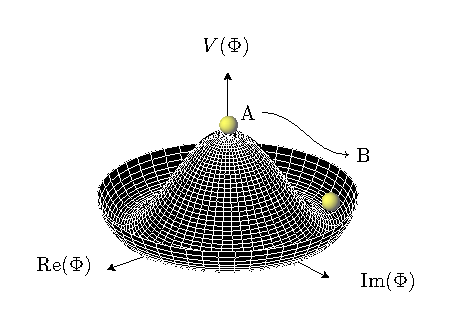
\includegraphics[width=.5\textwidth]{HiggsPotential/HiggsPotential}
			\caption{\label{fig:higgs_potential} The Higgs potential in the complex plane.} %Any given point around the bottom of the hat gives the lowest-energy state.}
			\end{wrapfigure}

			In summary, to generate particle masses gauge symmetry must be broken. However, in order for the theory to remain renormalisable, the global Lagrangian symmetry must be preserved. This can be solved introducing the concept of \emph{spontaneous} symmetry breaking (SSB): a mechanism that allows a symmetric Lagrangian, but not a symmetric VEV. In particular, given a Lagrangian invariant under a certain transformation, $T_X$ and a generic set of states, that transform under $T_X$ as the elements of a multiplet, the symmetry is spontaneously broken if one of those states is arbitrarily chosen as the ground state of the system. 
			%The Higgs-field VEV is not invariant under gauge transformations. In fact, it spontaneously breaks the gauge symmetry leaving the symmetry of the model untouched. 
			The interaction of the Higgs field with the $SU(2) \otimes U(1)$ gauge fields, $W_\mu^\alpha =1,2,3$, result in the three gauge bosons fields acquiring mass whilst the $B_0$ field stays massless. 





	\section{Limitations of the Standard Model}
	\label{sec:SMlim}

		During Run 1 and 2 of the LHC, the SM has been extensively validated, as shown in Fig. \ref{fig:ATLAS_a_SMSummary_TotalXsect}: the agreement, between the measured production cross section of various SM processes and the SM predictions, looks very good. However, the reasons behind the mass difference between the the three generations of fermions are still not explained by the SM because masses are treated as free parameters of the theory. In addition, there are some fundamental questions that have still no answer and they will be briefly discussed this section.

		\begin{figure}[!htb]
			\centering
			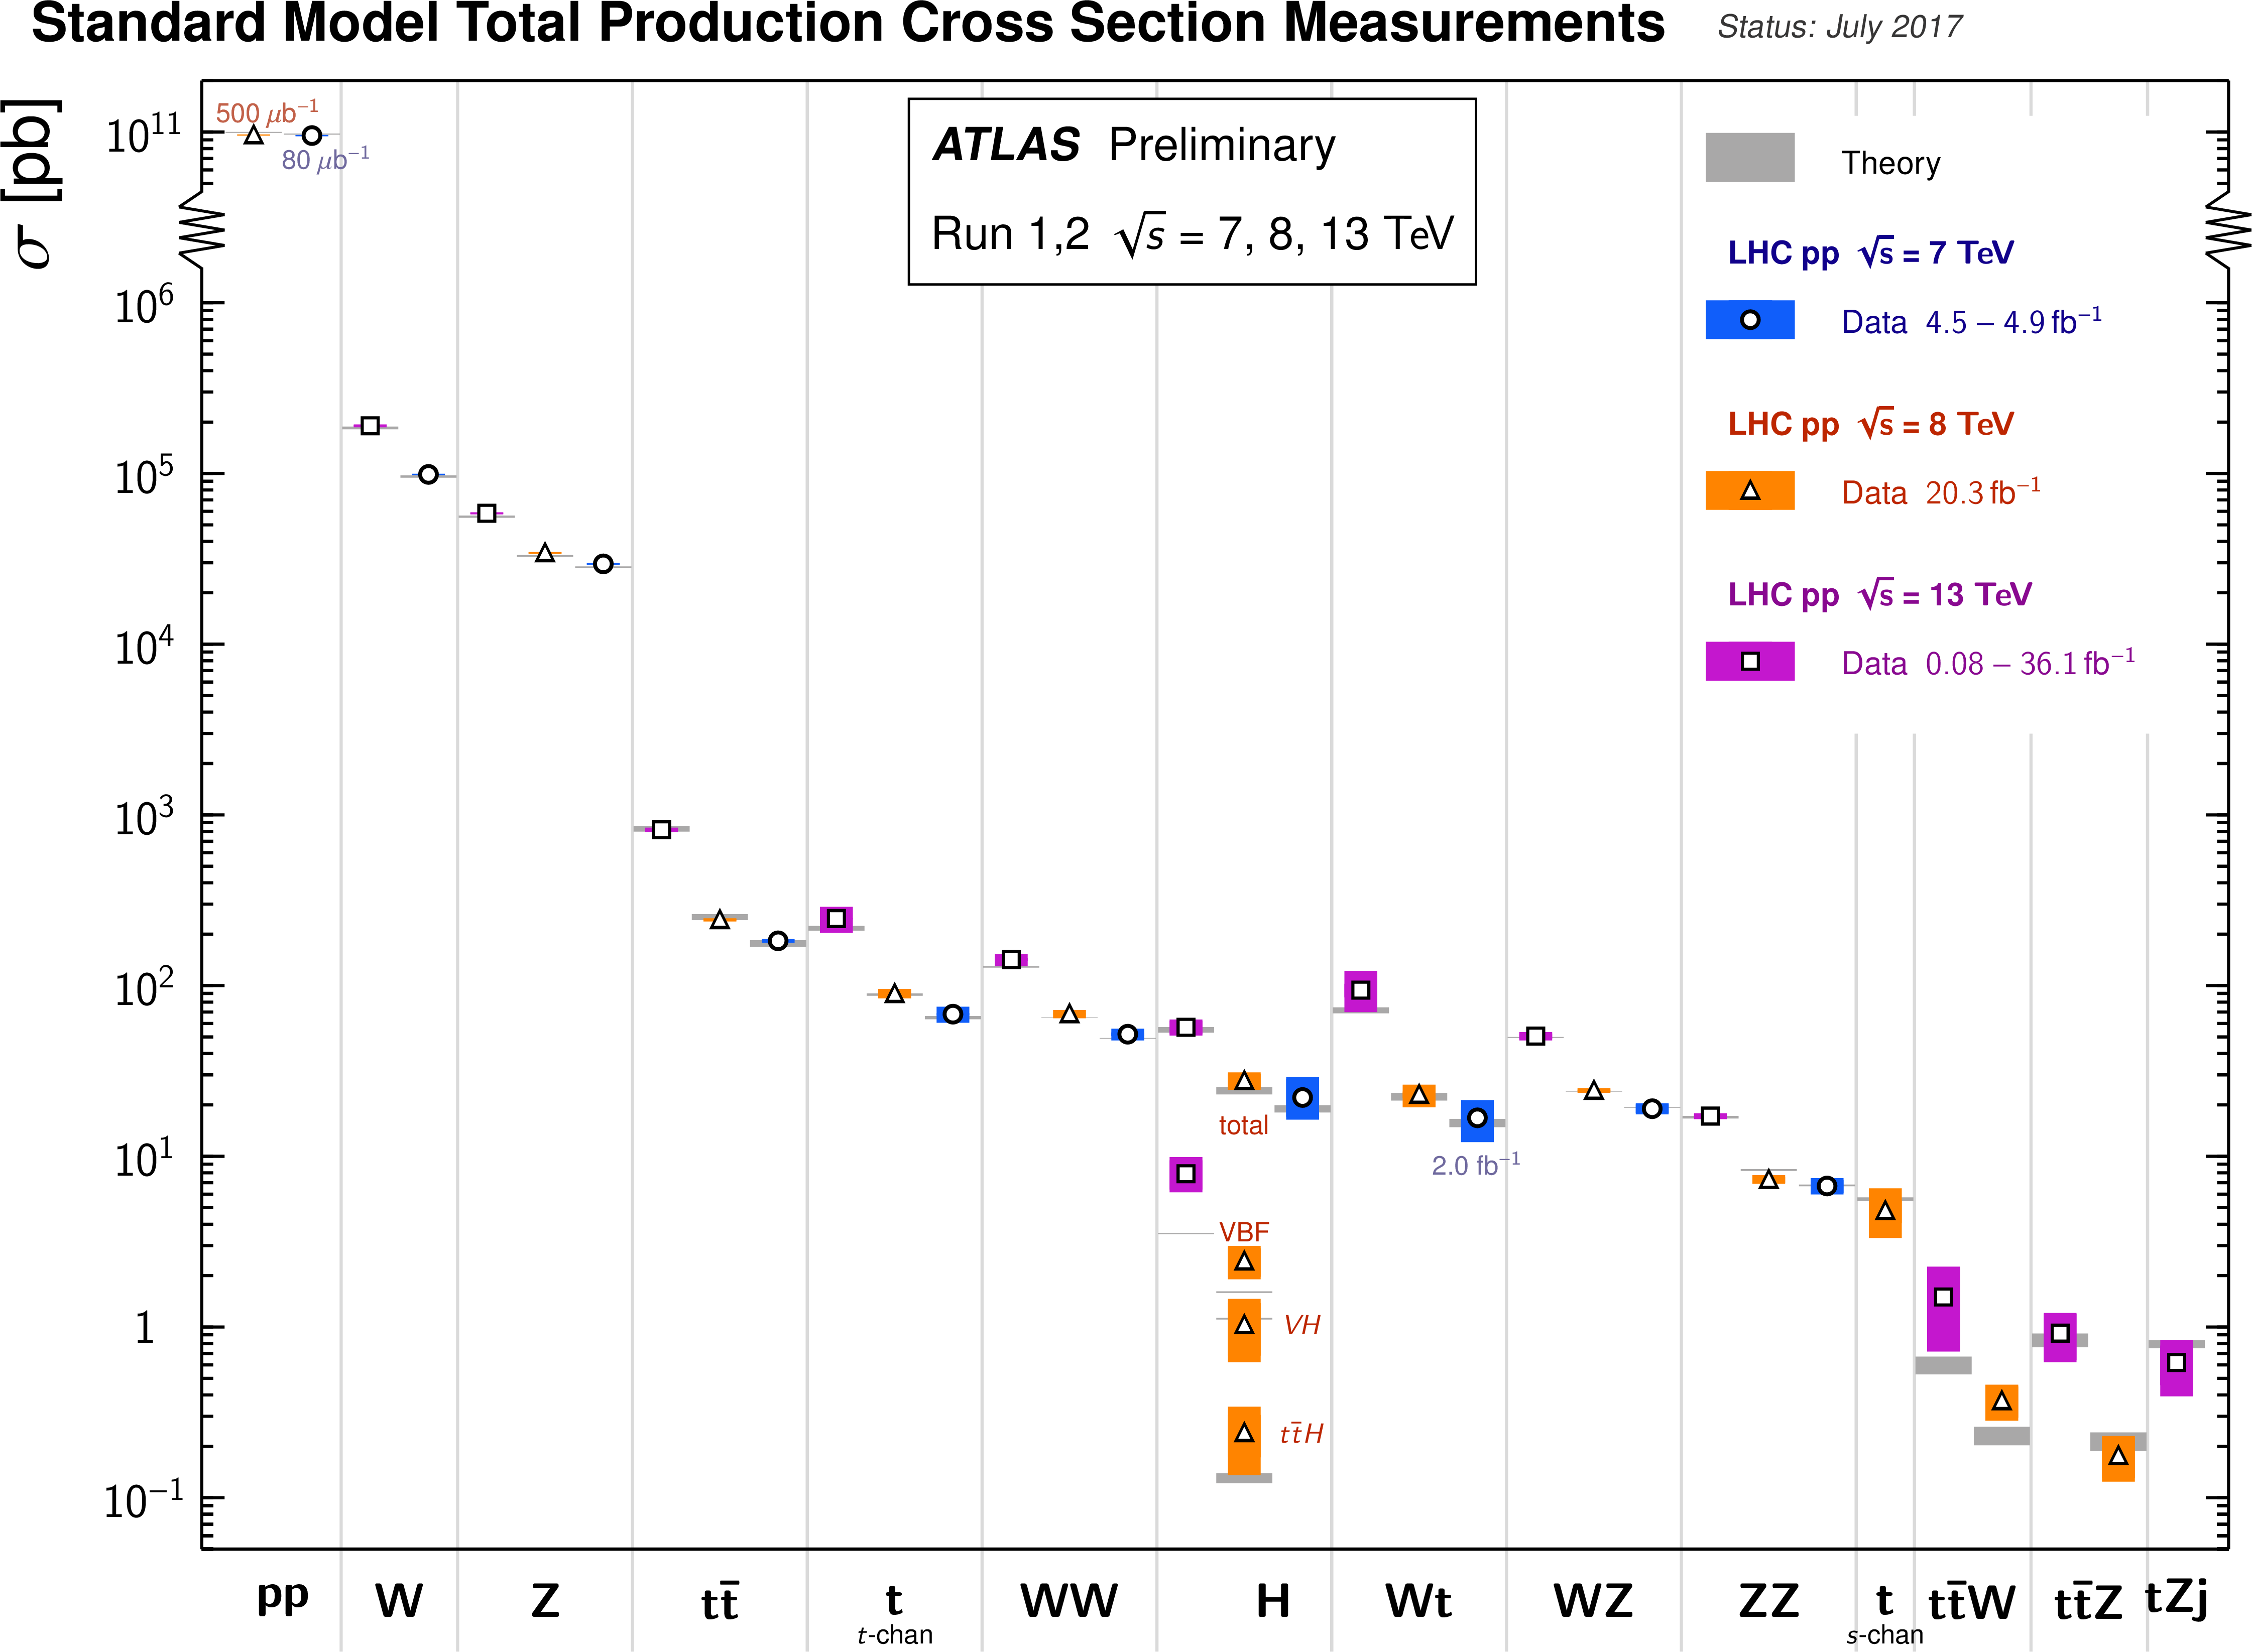
\includegraphics[width=\textwidth]{theory/ATLAS_a_SMSummary_TotalXsect}
			\caption{\label{fig:ATLAS_a_SMSummary_TotalXsect} Summary of several Standard Model total production cross section measurements, corrected for leptonic branching fractions, compared to the corresponding theoretical expectations. All theoretical expectations were calculated at NLO or higher. The luminosity used for each measurement is indicated close to the data point. Uncertainties for the theoretical predictions are quoted from the original ATLAS papers. They were not always evaluated using the same prescriptions for PDFs and scales. Not all measurements are statistically significant yet \cite{ATLAS_a_SMSummary_TotalXsect}.}
		\end{figure}



		\subsection*{Hierarchy Problem}

			Due to the coupling of every particle to the Higgs field, the one-loop corrections to the Higgs mass receive several contributions. 

			%\begin{wrapfigure}{l}{.\textwidth}
			\begin{figure}
				\centering
				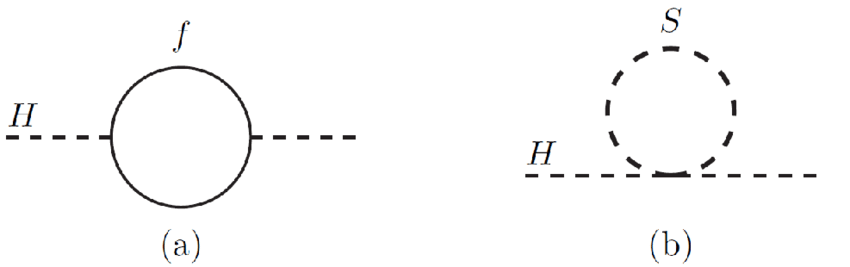
\includegraphics[width=.5\textwidth]{theory/1loopCorrectionsHM}
				\caption{\label{fig:higgs_coupling} One-loop quantum corrections to the Higgs mass: (a) a fermion correction with coupling $\lambda_f$ and (b) a scalar correction with coupling $\lambda_S$.}
			\end{figure}

			In particular, as shown in Fig. \ref{fig:higgs_coupling}:

			\begin{equation}
			\label{eq:mH_fermionic_contribution}
			\Delta m_H^2 = - \frac{ | \lambda_f  |^2}{8 \pi ^2} \Lambda_{\mathrm{UV}}^2 + \dots 
			\end{equation}

			\noindent which is the dominant, due to the fermionic contribution, and 

			\begin{equation}
			\label{eq:mH_scalar_contribution}
			\Delta m_H^2 = - \frac{\left | \lambda_S \right |^2}{16 \pi ^2} \left [  \Lambda_{\mathrm{UV}}^2 - 2m_S^2 \ln \left (\Lambda_{\mathrm{UV}} / m_S \right) + \dots \right ]
			\end{equation}

			\noindent due to the bosonic contribution. Here, $\lambda_f$ and $\lambda_S$ are the coupling to the fermionic field and the scalar field, respectively; $\Delta m_H^2$ is the difference between the observed Higgs mass $m_H^2$ and the bare mass, $m_H^0$ (Lagrangian parameter); $\Lambda_{\mathrm{UV}}$ is the ultraviolet momentum cut-off, selected to be at the Planck scale ($\sim 2 \cdot 10^{18} \gev$), at which a QFT description of gravity is believed to become possible. The correction to the Higgs mass then, will be around 30 orders of magnitude larger than Higgs mass itself, in opposition to what has been measured. This difference just mentioned, between the electroweak scale and the Planck scale arisen from the quantum corrections to the Higgs mass, is the so-called Hierarchy Problem \cite{Weinberg1976}.


		\subsection*{Neutrino Masses}

			The Super-Kamiokande Collaboration first, in 1998 \cite{SK1998}, and SNO Collaboration later, in 2001 \cite{SNO2001}, have provided measurements of the neutrino flux from solar and atmospheric sources. 
			The Nobel Prize in Physics 2015 was awarded jointly to Takaaki Kajita and Arthur B. McDonald ``for the discovery of neutrino oscillations, which shows that neutrinos have mass'' \cite{Nobel2015}. Such feature contraddicts the absence of a mechanism for mass generation for the neutrinos. 

			Various exotic solutions are on the market: one possible solution could be to add the so-called Majorana mass terms for the neutrino (seesaw mechanism). Neutrino physics could unveil physics beyond the SM.



		\subsection*{Dark Matter}

			Although dark matter (DM) has never been directly observed, its existence is inferred from its gravitational effects. For example, looking at galaxies rotation, it was observed that the rotation speed was higher than expected, given the amount of visible matter. Two different reasoning arose during the last century to justify such effect either there is matter that cannot be seen by us (in terms of visible light), which contributes to the galatcis mass; or the general relativity works differently at galactic distances. The former is believed to be the most likely and it implies the existence of new particles which do not interact via electromagnetic interaction, the so-called Weakly Interacting Massive Particles (WIMPs).





	\section{Supersymmetry}
	\label{sec:SUSY}

		Supersymmetry links gravity with the other fundamental forces of nature by introducing a space-time symmetry that relates bosons to fermions and vice-versa, via a transformation of the form of:  

		\begin{equation}
		\label{eq:susy_transformation}
			Q \ket{\mathrm{fermion}} = \ket{\mathrm{boson}}, \qquad Q \ket{\mathrm{boson}} = \ket{\mathrm{fermion}}
		\end{equation}

		\noindent For each SM particle there exists a superpartner with a spin difference of $\Delta s = 1/2$. As of today, superpartners, generally called \emph{sparticles} (where the \emph{s} stands for ``scalar''), have not been observed yet, resulting in the assumption that SUSY must be a broken symmetry, otherwise superpartners would have the same quantum numbers and masses as their SM equivalent. However, if sparticles were to be too heavy (close to the Planck scale), the hierarchy problem would still remain unsolved. The \emph{soft} SUSY breaking mechanism overcomes this problem imposing contrains on the masses of sparticles to a range that can be experimentally explored. 

		In this section an overview of Supersymmetry (SUSY) will be presented, together with the motivations behind the success of such theory. Third generation SUSY will be also discussed as it is the most relevant theoretical support to the analyses presented in Chapter \ref{ch:stop_ana}. 
		

		\subsection{Why SUSY?}


			

		\subsection{SUSY Models}


		\subsection*{Minimal Supersymmetric Standard Model}
			
			bla

		\subsection*{\emph{R}-parity SUSY}
		
			bla

		\subsection*{Simplified models}
		
			bla


		\subsection*{Phenomenological MSSM}
		
			bla

		\subsection{Third generation Supersymmetry}


        \chapter{The ATLAS Experiment at the LHC}
\epigraph{\emph{We are rather like children, who must take a watch to pieces to see how it works}}{Sir Ernest Rutherford}

	ATLAS (A Toroidal LHC ApparatuS) is one of the four main experiments (ATLAS, CMS, ALICE, LHCb) taking data at a center-of-mass energy of $13$ TeV using beams delivered by the Large Hadron Collider (LHC). In this chapter an overview of the LHC will be given in Section~\ref{sec:lhc}, then the ATLAS detector will be described in Section~\ref{sec:det}, and finally the Trigger system, used to cleverly store the data, will be described in Section~\ref{sec:trigSyst}. A more in-depth description of the Trigger algorithms I have been involved in will be given in Chapter~\ref{ch:trigger}.



	% --------------------------------
	% -------  THE LHC
	% --------------------------------
	\section{The LHC}
	\label{sec:lhc}
	
		As of today, the LHC is the world’s largest and most powerful particle accelerator. It was designed to help answer some of the fundamental open questions in particle physics by colliding protons at an unprecedented energy and luminosity. It is located at the European Organisation for Nuclear Research (CERN), in the Geneva area, at a depth ranging from 50 to 175 metres underground. It consists of a 27-kilometre ring made of superconducting magnets, and inside it two high-energy particle beams travel in opposite directions and in separate beam pipes. 

		The beams are guided around the ring by a strong magnetic field generated by coils - made of special electric cables - that can operate in a superconducting regime.%, being capable of conducting electricity almost without resistance or loss of energy. 
		1232 superconducting dipole and 392 quadrupole magnets, with an average magnetic field of 8.3 T, are employed and kept at a temperature below 1.7 K, in order to preserve their superconducting properties. The formers are used to bend the beams and the latters to keep them focused while they get accelerated. 
		%In order for this to be possible though, the magnets have to remain at a temperature of -271.3$^\circ$C for which a distribution system of liquid helium is employed.
		
		The collider first went live on September 2008 even though, due to a magnet quench incident that damaged over 50 superconducting magnets, it has been operational since November 2009 when low-energy beams circulated in the tunnel for the first time since the incident. This also marked the start of the main research programme and the beginning of the so-called Run 1: first operational run (2009 - 2013).


		%\subsection*{Performance of the LHC}
		\subsection*{Performance of the LHC}

			In June 2015 the LHC restarted delivering physics data, after a two-year break, the so-called Long Shutdown 1 (LS1), during which the magnets were upgraded to handle the current required to circulate 7-TeV beams. It was the beginning of the so-called Run 2 - second operational run (2015-2018) - during which LHC has collided up to $10^{11}$ bunches of protons every 25 ns at the design luminosity - the highest luminosiy the detector was designed to cope with - of $2 \cdot 10^{34} \mathrm{cm}^{-2}\mathrm{s}^{-1}$. The definiton of the luminosity is:

			\begin{equation}
				{\mathcal L} = f \frac{n_b N_1 N_2}{4 \pi \sigma_x \sigma_y}
			\label{eq:lumi}
			\end{equation}

			\noindent where $N_1$ and $N_2$ are the number of protons per bunch in each of the colliding beams, $f$ is the revolution frequency of the bunch collisions, $n_b$ the number of proton per bunch, and $\sigma_x$ and $\sigma_y$ are the horizontal and vertical dimensions of the beam. The luminosity is strictly related to the number of collisions occurring during a certain experiment via the following: 

			\begin{equation}
					{\mathcal N}_{\mathrm{event}} = {\mathcal L} \sigma_{\mathrm{event}}
			\label{eq:lumiEvt}
			\end{equation}

			\noindent where $\sigma_{\mathrm{event}}$ is the cross section of the process under investigation.  It has not only collided protons but also heavy ions, in particular lead nuclei at $\sqrt{s_{NN}} = 5.02$ TeV, at a luminosity of $10^{27} \mathrm{cm}^{-2} \mathrm{s}^{-1}$\cite{HI2015}.



		\subsection*{Acceleration stages}

			\begin{figure}[!htb]
				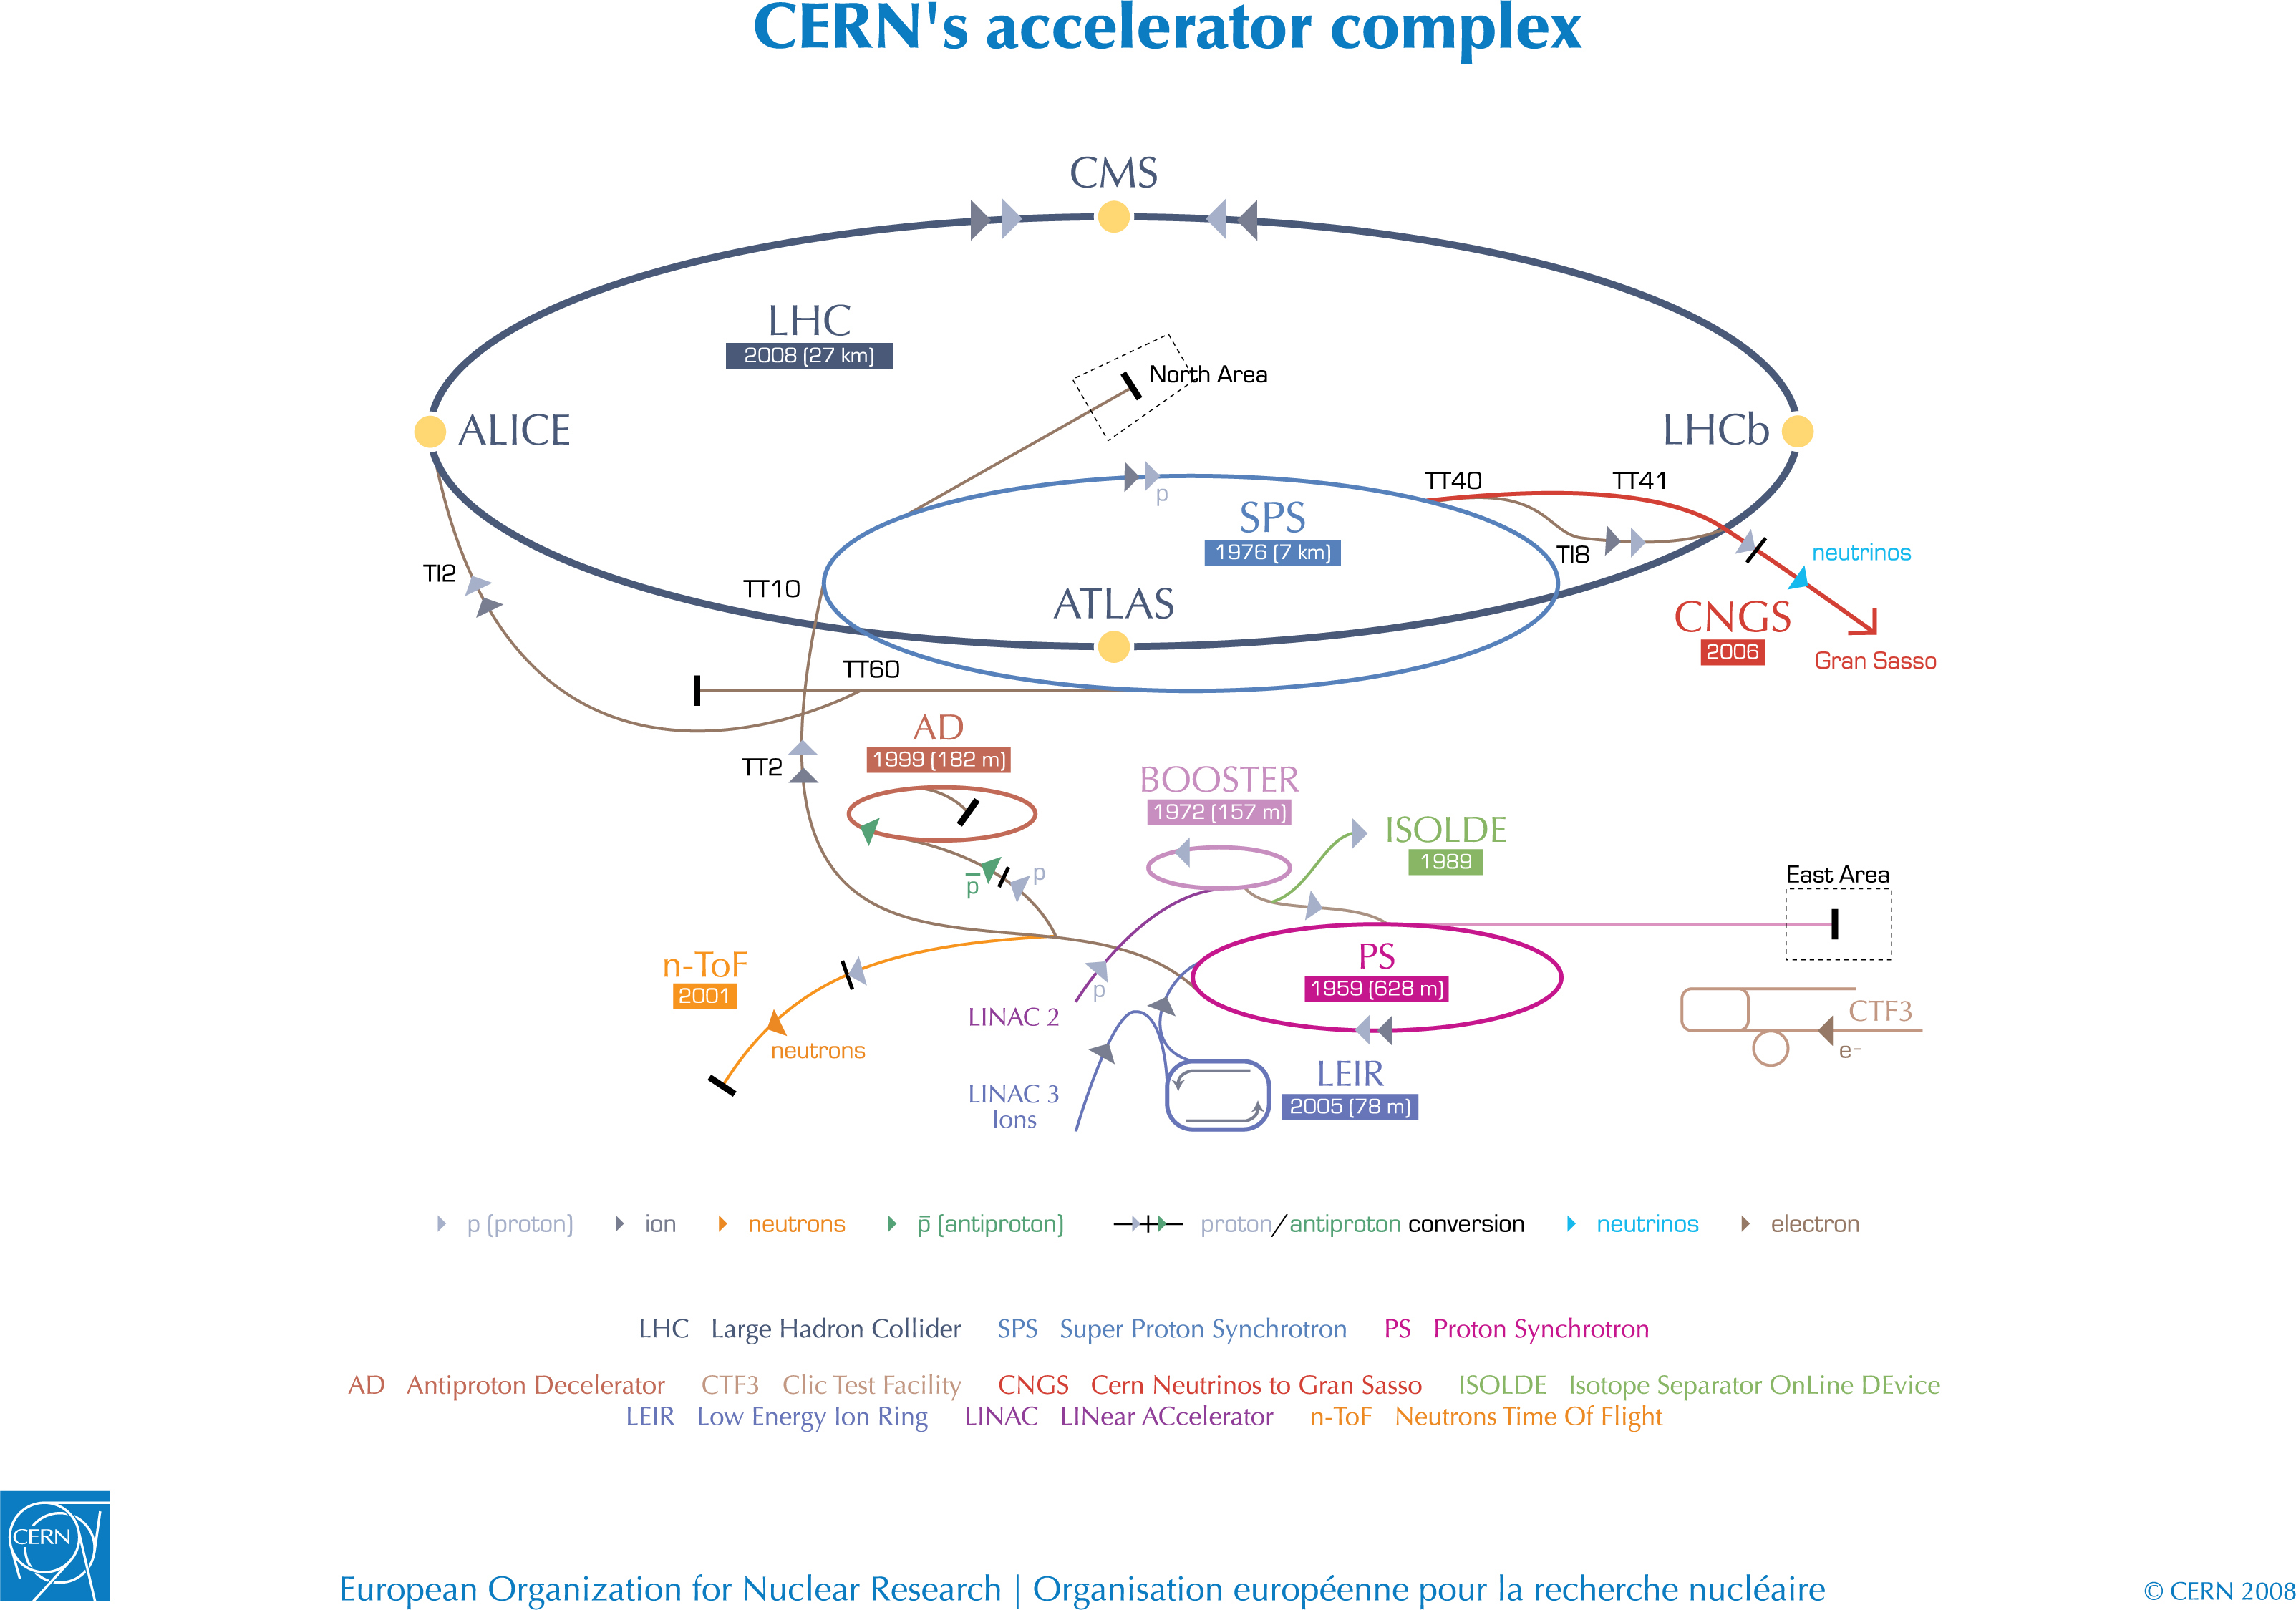
\includegraphics[width=\textwidth]{Detector/cern-acc-complex.jpg}
				\caption{CERN Accelerator complex. The LHC is the last ring (dark grey line). Smaller machines are used for early-stage acceleration and also to provide beams for other experiments~\cite{Lefevre2008}.}
				\label{fig:cern-acc-complex}
			\end{figure}

			Before reaching the maximum energy, the proton beams are accelerated by smaller accelerators through various stages. Figure~\ref{fig:cern-acc-complex} shows a sketch of the CERN's accelerator complex. It all begins at the linear accelerator LINAC 2. Here protons are accelerated up to 50 MeV, and then injected in the Proton Synchrotron Booster (PSB) where they reach 1.4 \GeV. The next stage is the Proton Synchrotron (PS), which boosts the beams up to 25 \GeV\, and then the Super Proton Synchrotron (SPS) makes them reach energies up to 450 \GeV. Eventually, the beams are injected in bunches with a 25 ns spacing into the LHC, where they travel in opposite directions, while they are accelerated to up to 13 TeV. Once the bunches reach the maximum energy, they are made collide at four different points, inside four experiments around the ring~\cite{LHCDesignReport}. 

			The heavy ion beams acceleration procedure is slightly different. Their journey starts at LINAC 3 first, and the Low Energy Ion Ring (LEIR) then, before they make their way into the PS where they follow the same path as the protons~\cite{LHCDesignReport}. 

			The four large detectors on the collision points are; the multi-purpose detectors A Toroidal LHC ApparatuS (ATLAS), and Compact Muon Solenoid (CMS)~\cite{CMSJINST}, Large Hadron Collider beauty (LHCb)~\cite{LHCb2008}, which focuses on flavour physics, and A Large Ion Collider Experiment (ALICE)~\cite{ALICEJINST} which specialises in heavy ion physics. The \emph{big four} are not the only experiments at the CERN's accelerator complex. There also are smaller experiments based at the the four caverns about the collision points e.g. TOTEM, LHCf and MoEDAL, but this will not be discussed any further in this thesis.
		


	% --------------------------------
	% -------  THE DETECTOR
	% --------------------------------
	\section{The ATLAS Detector}
	\label{sec:det}

		\begin{figure}[!htb]
			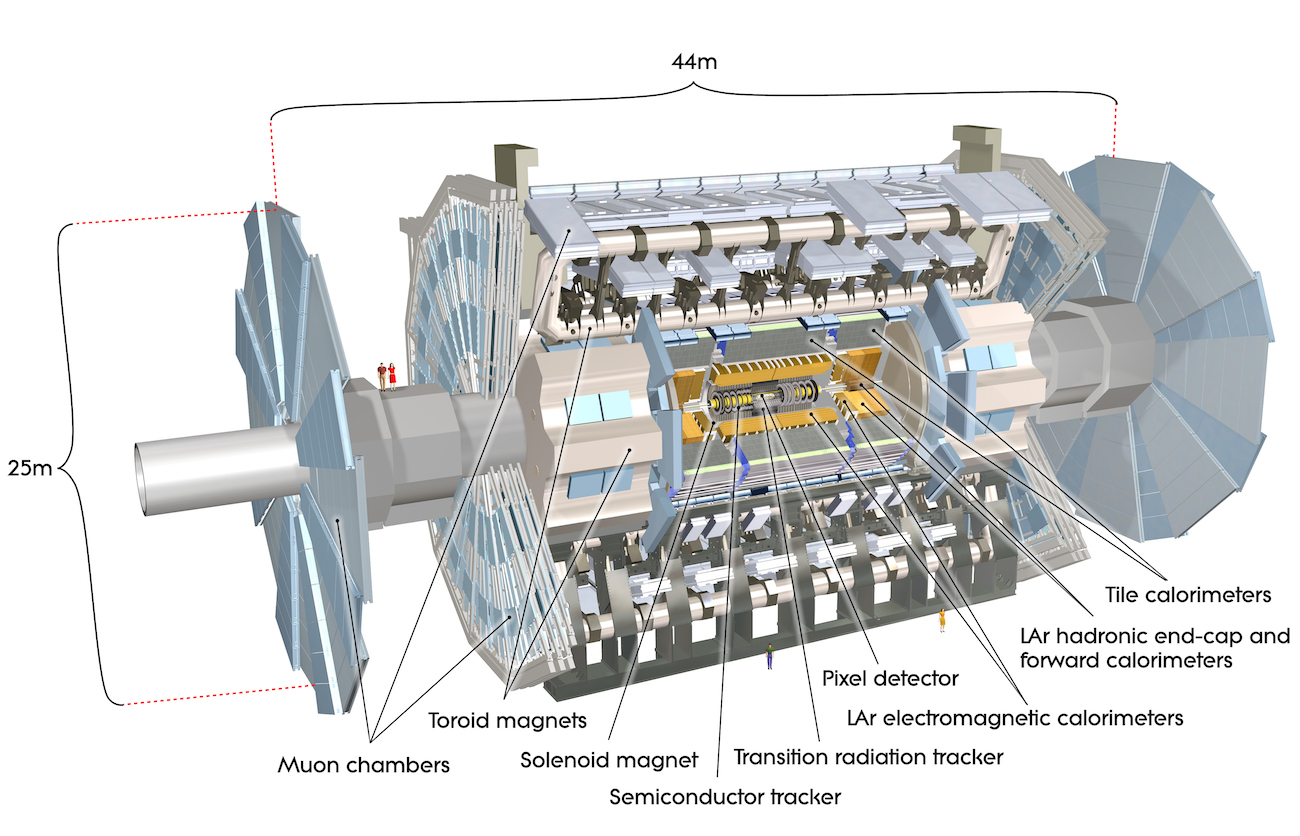
\includegraphics[width=\textwidth]{Detector/cut-away-det.jpg}
			\caption{Cut-away view of the ATLAS detector. The dimensions of the detector are 25 m in height and 44 m in length. The overall weight of the detector is approximately 7000 tonnes~\cite{Lefevre2008}.}
			\label{fig:cut-away-det}
		\end{figure}


		ATLAS is a general-purpose detector designed to collect data with the highest luminosity provided by the LHC. It is located at CERN's Point 1 cavern and it measures about 45 m in length and 25 m in diameter. It has a forward-backward symmetric cylindrical geometry with respect to the interaction point and it is designed to reconstruct and measure physics objects such as elctrons, muons, photons and hadronic jets. Its design was optimised to be as sensitive as possitble to the discovery of the Higgs boson and beyond-the-Standard-Model (BSM) physics. In fact, thanks to the other sub-systems, ATLAS is able to observe all possible decay products by covering nearly $4\pi$ steradians of solid angle.

		In Figure~\ref{fig:cut-away-det} a cut-away view of ATLAS with all its components is shown. The innermost layer is the Inner Detector (ID) which is the core of the tracking system and consists of a Pixel, a Silicon micro-strip tracker (SCT), and a Transition Radiation Tracker (TRT). It is submerged in a 2 T magnetic field, generated by a thin superconducting solenoid, which bends all the charged particles' trajectories allowing transverse momemtum measurement. The electromagnetic and hadronic calorimeters form the next layer and they are both used to perform precise energy measurements of photons, electrons, and hadronic jets. Finally, the outermost layer corresponds to the Muon Spectrometer (MS) which, together with the ID, enclosed in a toroidal magnetic field, allows precise measurement of momentum and position of muons. These sub-detectors will be discussed in more detail in the following sections. 
	

		% --------------------------------
		% -------  THE GEOMETRY
		% --------------------------------
		\subsection*{The ATLAS coordinate system}
		\label{par:coord}
			
			A coordinate system is taken on for the spatial definition of the sub-systems %the definition of the above-mentioned physics object reconstruction, 
			and kinematic measurement of physics processes. Such system is defined starting from the interaction point, defined as the origin. The $z$-axis is defined by the beam direction and the $x-y$ plan, as transverse to the beam direction.

			A quantity, known as pseudorapidity, ($\eta$), is defined to describe the angle of a particle coming out of the collision, with respect to the beam axis: 

			\begin{equation*}
				\eta \equiv -\ln (\tan(\theta/2))
			\end{equation*}

			\noindent Here $\theta$ is the polar angle. The azimuthal angle, $\phi$, is defined around the beam axis and the polar angle. In the $(\eta,\phi)$ space a distance $\Delta R$ can be therefore defined as  
			
			\begin{equation*}
				\Delta R = \sqrt{{\Delta \eta}^2 + {\Delta \phi}^2}
			\end{equation*}

			\noindent where $\Delta \eta$ and $\Delta \phi$ are the differences in pseudorapidity and azimuthal angle between any two considered objects. A central and a forward region of pseudorapidity are also defined such that the detector components are described as part of the \emph{barrel} if they belong to the former or as part of the \emph{end-caps} if they belong to the latter. 



		% --------------------------------
		% -------  THE MAGNET
		% --------------------------------
		\subsection{The Magnet System}
		\label{sec:magnet-system}
			
			\begin{figure}[!htb]
				%\centering
				\subfloat[Geometry of magnet windings and tile calorimeter steel. The eight barrel toroid coils, with the end-cap coils interleaved are visible. The solenoid winding lies inside the calorimeter volume~\cite{ATLASJINST}.]
				{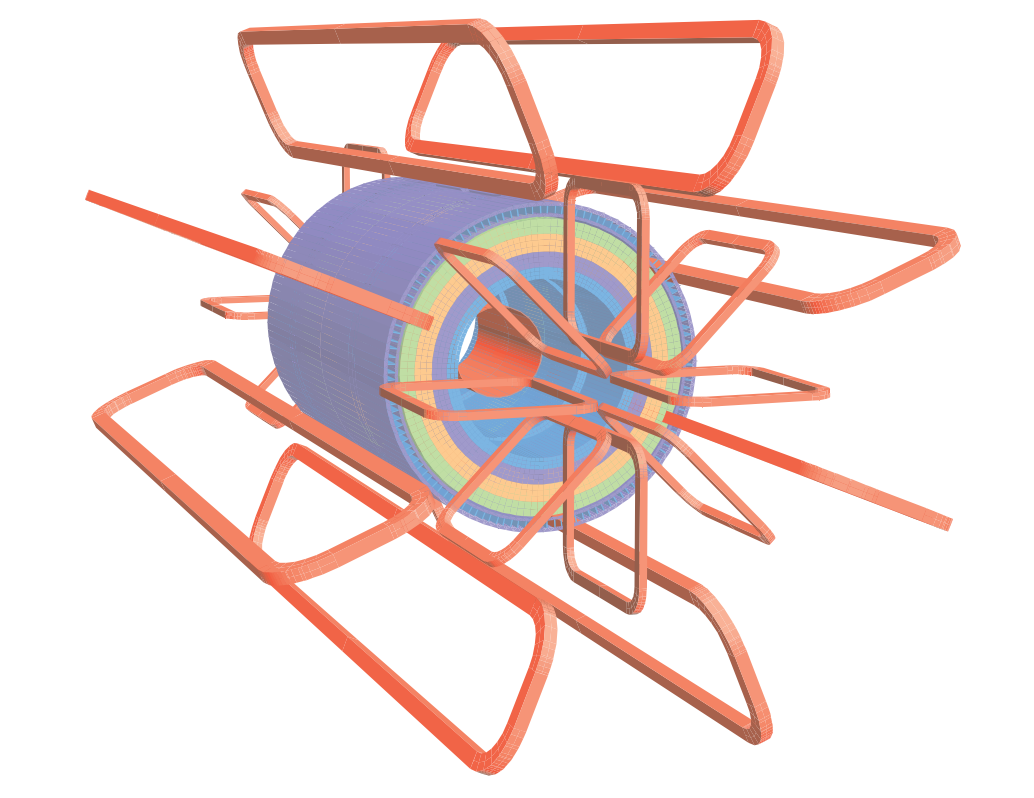
\includegraphics[width=0.475\textwidth]{Detector/MagnetSyst/magnetSyst}\label{fig:magnetSyst}}
				\hfill
				%\centering
				\subfloat[Schematic view of the superconducting magnets~\cite{YAMAMOTO200853}.]
				{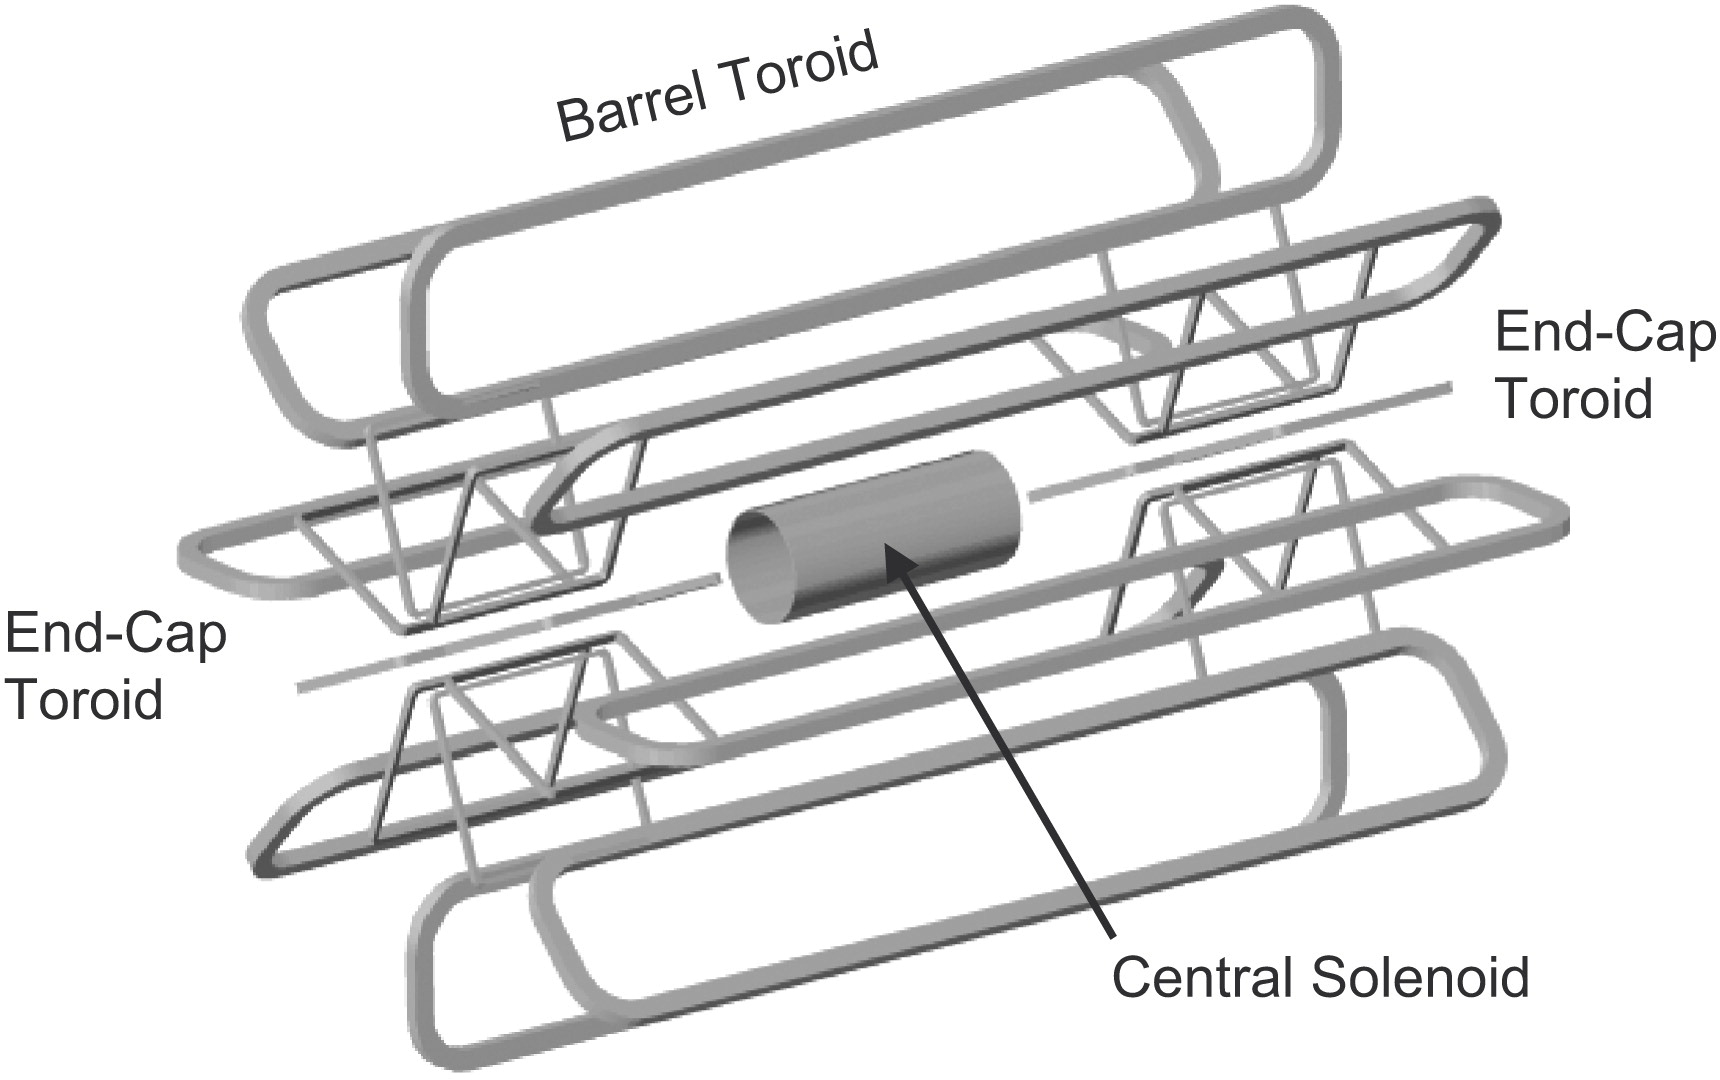
\includegraphics[width=0.475\textwidth]{Detector/MagnetSyst/magnetSyst-desc}\label{fig:magnetSyst-desc}}
				\caption{The ATLAS magnet system.}
			\end{figure}

			\noindent The ATLAS magnet system, 26 m long with a 22 m diameter, generates the magnetic field needed to bend the trajectories of charged particles in order to perform momentum measurement. Figure~\ref{fig:magnetSyst} and~\ref{fig:magnetSyst-desc} show the geometry of the system and its components, which are made of NbTi - superconducting material - and will be described in the following parahraphs. 



			\subsection*{The Central Solenoid}

				With an axial length of 5.8 m, an inner radius of 2.46 m, and an outer radius of 2.56 m, the central solenoid magnet is located between the ID and the ECAL. Its function is to bend the charged particles that go through the ID and it is aligned on the beam axis providing a 2 T axial magnetic field that allows accurate momentum measurement up to 100 \GeV~\cite{YAMAMOTO200853}.

			\subsection*{The Barrel and the End-cap Toroids}

				Figure~\ref{fig:magnetSyst-desc} displays the toroid magnetic system that surrounds the calorimeters. With its cylindrical shape this component consists of a barrel and two end-caps toroids, each with eight superconducting coils. The system allows accurate measurement of muon momenta using a magnetic field of approximately 0.5 T (barrel) for the central regions and 1 T (end-cap) for the end-cap regions, respectively, which bends the particles in the $\theta$ direction.

				
		% --------------------------------
		% -------  THE ID
		% --------------------------------
		\subsection{The Inner Detector}
		\label{sec:ID}

			The Inner Detector (ID)~\cite{ATLASInDet} is the innermost component of the ATLAS detector \ie\ the nearest sub-detector to the interaction region and it is used to reconstruct charged particle tracks used in the selection of physics objects. In fact, it allows robust track reconstruction, with accurate impact parameter resolution ($\sim 20 \mu m$) and precise primary and secondary vertex reconstruction for charged particles (tracks) above 500 \MeV\ and within $\displaystyle|\eta| < 2.5$.

			\begin{figure}[!htb]
				\subfloat[Overview of the ATLAS ID with labels and dimensions.]{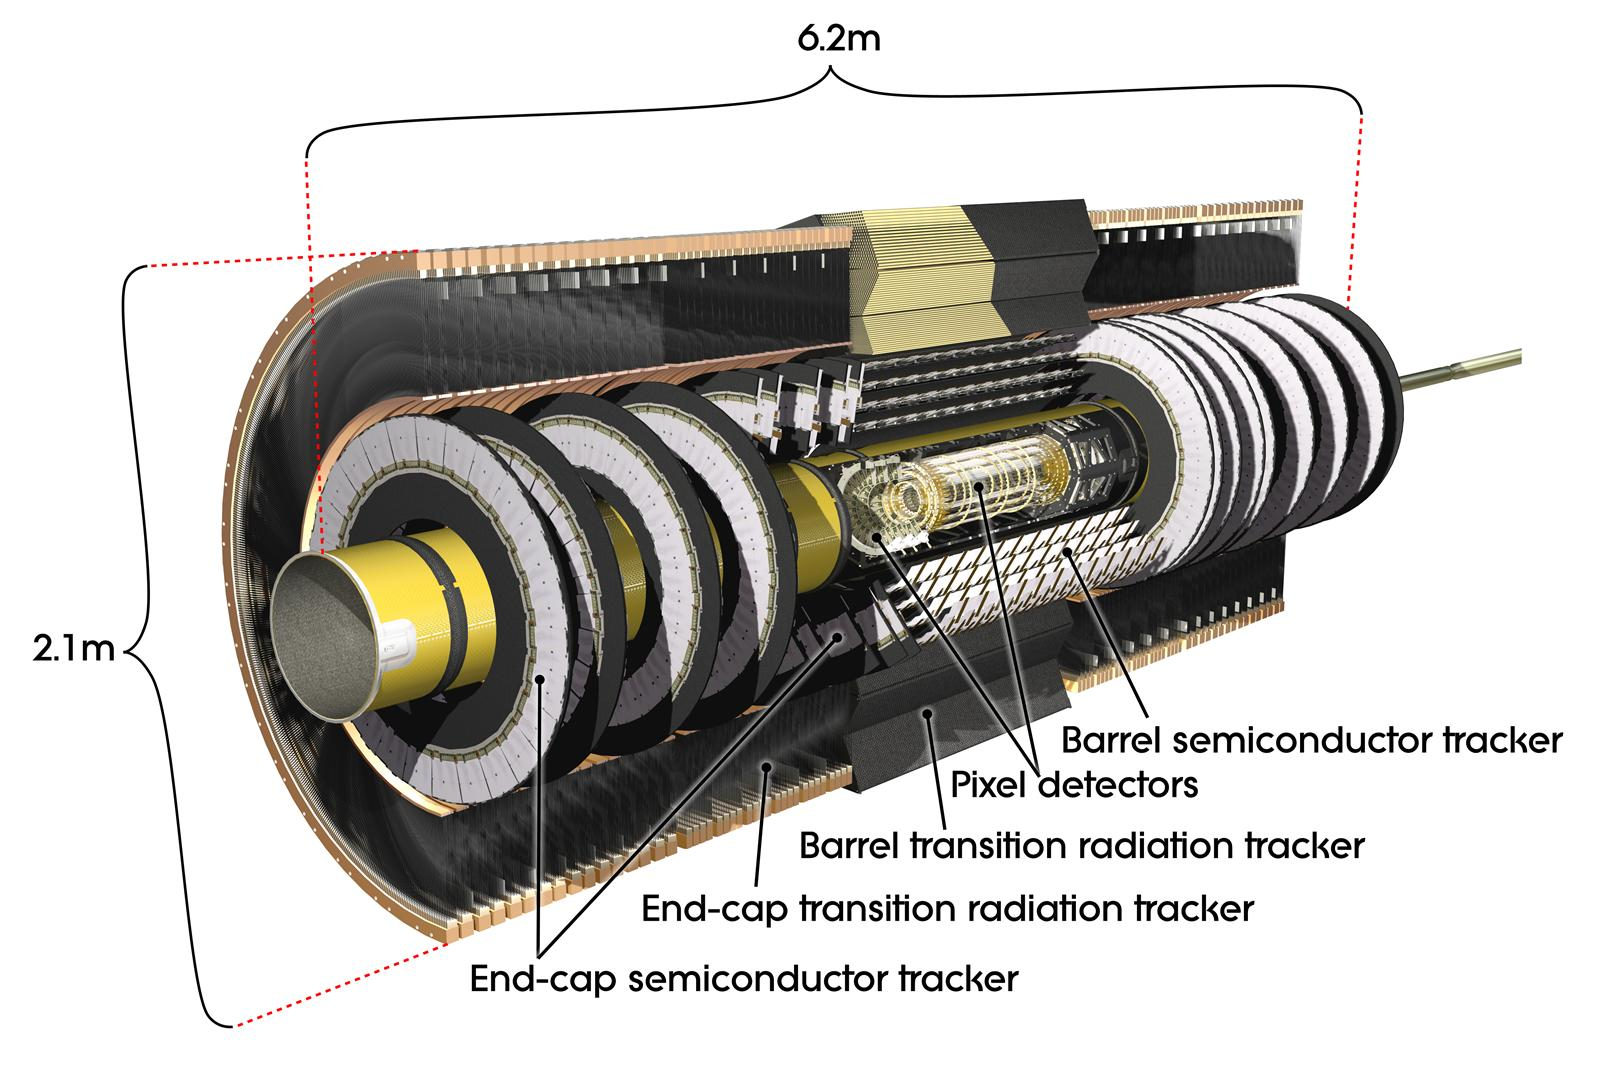
\includegraphics[width=0.475\textwidth]{Detector/ID/ID-overview}\label{fig:ID-overview}}\hfill
				\subfloat[Diagram of the ATLAS ID and its sub-detectors.]{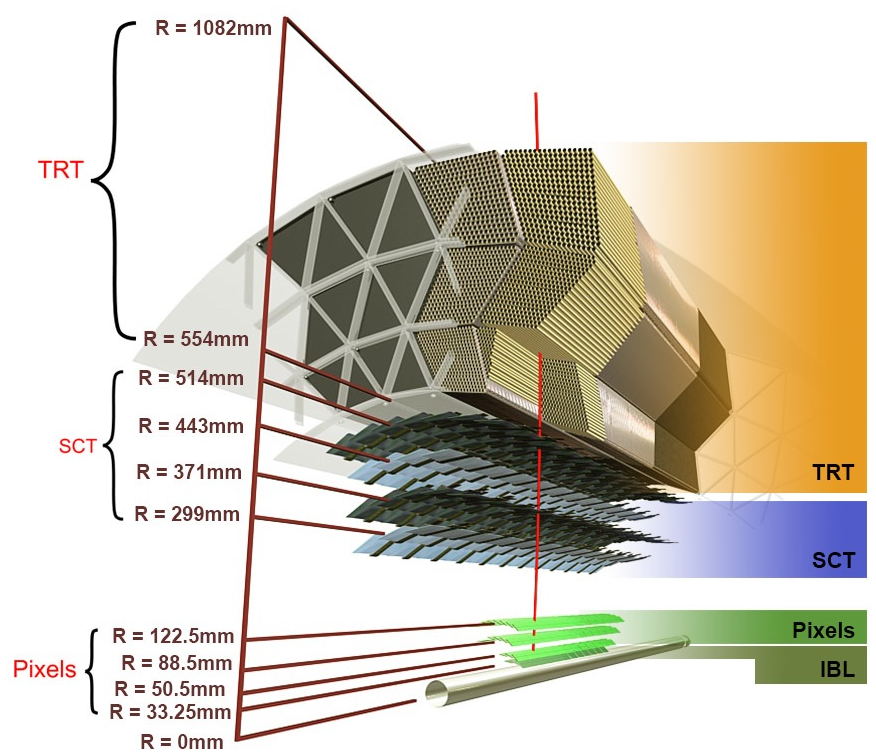
\includegraphics[width=0.475\textwidth]{Detector/ID/ID}\label{fig:ID}}
				\caption{The ATLAS Inner Detector}
				\label{fig:AID}
			\end{figure}


			The ID is comprised of independent and concentric sub-systems, which are all shown in Figure~\ref{fig:AID}: %\ref{fig:ID} and~\ref{fig:ID-overview}:

			\begin{itemize}
				\item \underline{Insertable B-Layer (IBL):} \\innermost Pixel Detector layer added during ATLAS Run 2 upgrade (2013/2014) to improve vertexing and impact parameter reconstruction;
				\item \underline{Silicon Pixel Tracker (Pixel):} \\made of silicon pixel layers and used mainly for reconstructing both the primary and secondary vertices in an event;
				\item \underline{SemiConductor Tracker (SCT):} \\comprised of silicon microstrip layers; thanks to its resolution ($17 \times 580\, \mu$m) it can accurately measure particle momenta;
				\item \underline{Transition Radiation Tracker (TRT):} \\final layer comprised of various layers of gaseous straw tube elements surrounded by transition radiation material.
			\end{itemize}

			These sub-detectors will be discussed in the following sections.  

			\subsection*{IBL} 
				
				The IBL~\cite{IBLTDR} is the innermost Pixel Detector layer as shown in Figure~\ref{fig:ID}. It is comprised of 6M channels and each pixel measures $50 \times 250\,\mu$m. Its resolution is $8 \times 40\, \mu$m,The addition of this new layer brought a considerable improvement on the performance of the Pixel Detector by enhancing the quality of impact parameter reconstruction of tracks. In particular, this was achieved by improving the vertex finding efficiency and the tagging of bottom-quark-initiated jets (\emph{b}-jets) which, in case of a B-layer failure, can be restored by the IBL. Besides these improvements, the IBL insertion allowed ATLAS to better cope with high luminosity effects such as the increase in event pile-up, which leads to high occupancy and read-out inefficiency. 

			\subsection*{Pixel}
				
				The Pixel detector is comprised of 1750 identical sensorchip-hybrid modules, each covering an active area of 16.4 $\times$ 60.8 mm. The total number of modules correspond to roughly 80 million semiconductor silicon pixels. The nominal pixel size is 50 $\mu$m in the $\phi$ direction and 400 $\mu$m in the barrel region, along the $z$-axis (beam axis)~\cite{ATLASPix}. The reason why such a large amount of pixels is employed is justified by the need to cope with the high luminosity in ATLAS. The silicon pixel detector measures 48.4 cm in diameter and 6.2 m in length providing a pseudorapidity coverage of $\left|\eta\right| < 2.5$. Figure~\ref{fig:ID} shows the three concentric barrel layers placed at 50.5 mm, 88.5 mm and 122.5 mm respectively. Furthermore, the Pixel detector is made of six disk layers, three for each forward region, such that when a charged particle crosses the layers it will generate a signal at least in three space points. The fine granularity of such detector allows accurate measurement and precise vertex reconstruction, as it provides a more accurate position measurement as a large detection area is available. In particular, it has a resolution of $10 \times 115\,\mu$m.

			\subsection*{SCT}

				The SCT is made of 4088 modules of silicon micro-strip detectors arranged in four concentric barrel layers. It is mainly used for precise momentum reconstruction over a range $\left|\eta\right| < 2.5$ and it was designed for precision measurement of the position using four points (corresponding to eight silicon layers), obtained as track hits when crossing the layers. Figure~\ref{fig:ID} shows the structure of the SCT with its four concentric barrel layers with radii ranging from 299 mm to 514 mm and two end-cap layers. Each module has an intrinsic resolution of 17 $\mu$m in the $R-\phi$ direction and 580 $\mu$m in the $z$ direction. As the SCT is further away from the beam-pipe than the Pixel detector, it has to cope with reduced particle density. This allows for reduced granularity mantaining the same level of performance of the Pixel detector: SCT can use $\sim$ 6.3 million read-out channels.%, almost 2 million fewer than the pixel detector.


			\subsection*{TRT}
			 
				The last and outermost of the sub-systems in the ID is the TRT. It is a gaseous detector which consists of 4 mm diameter straw tubes wound from a multilayer film reinforced with carbon fibers and containing a 30 $\mu$m gold plated tungsten wire in the center. The straw is filled with a gas mixture of 70\% Xe, 27\% CO$_2$ and 3\% O$_2$~\cite{TRT2012}. As shown in Figure~\ref{fig:ID}, its section consists of three concentric layers with radii ranging from 544 mm to 1082 mm, each of which has 32 modules containing approximately 50,000 straws, 1.44 m in length, aligned parallel to the beam direction with independent read-out at both ends. Both end-cap sections are divided into 14 wheels, with roughly 320,000 straws in the R-direction. The average 36 hits per track in the central region of the TRT allow continuous tracking to enhance pattern recognition and momentum resolution in the $\left| \eta \right| < 2.5$ region. It also improves the \pt\ resolution for longer tracks.



		% --------------------------------
		% -------  THE CALORIMETERS
		% --------------------------------
		\subsection{The Calorimeters}

			\begin{figure}[!htb]
				\centering
				\includegraphics[width=\textwidth]{Detector/Calo/Calo-overview}
				\caption{A computer generated image of the full calorimeter.}
				\label{fig:Calo}
			\end{figure}

			The ATLAS Calorimeter system, shown in Figure~\ref{fig:Calo}, is comprised of two main sub-systems; the electromagnetic calorimeter (ECAL) and hadronic calorimeter (HCAL), which are designed to stop and measure the energy of electromagnetic-interacting and hadronic particles respectively. The combination of the two provides full coverage in $\phi$ and $\left | \eta \right | < 4.95$. Particles slow down and lose energy generating showers when crossing different layers. The ECAL is comprised of one barrel and two end-cap sectors employing liquid Argon (LAr). The showers hereby develop as electrons pairs which are then collected. The HCAL is also comprised of one barrel and two end-cap sectors. The sensors in the barrel of the HCAL are tiles of scintillating plastic whereas LAr is employed for the end-cap. A forward region, the closest possible to the beam, is covered by a LAr forward calorimeter (FCal). The LAr and Tile Calorimeter will be briefly discussed in the following parapgraphs. 
			%The particles have to deposit all their energy within the calorimeters to obtain an accurate energy measurement and avoid energy deposits in the outer muon spectrometer.
			%The definitions of radiation length ($X_0$), the distance over which an electron loses 1/$e$ of its energy within a given material, and nuclear interaction length ($\lambda_I$), are used to define the lengths of the barrel and the endcap regions of the calorimeter system. The ECAL roughly measures 22 $X_0$ thick in the region of barrel, and 24 $X_0$ in the end caps. The HCAL roughly measures 10 $\lambda_I$. Both ECAL and HCAL measures vary with $\eta$. Furthermore, it is known that hadronic particles are more penetrating than the electromagnetic ones and in particular, $\lambda_I$ is roughly ten times bigger than $X_0$. 

			\subsection*{The Liquid Argon Calorimeters}

 				The ECAL is comprised of multiple layers of liquid Argon (LAr) sampler and lead absorber. The choice of its accordion-geometry design brought two main advantages; full $\phi$ coverage with no non-interactive regions (no cracks); fast extraction of signals coming from both front or rear end of the electrodes. It is made of two half-barrel wheels, both placed in the barrel cryostat, that provide a pseudorapidity coverage up to $\left | \eta\right | < 1.475$ and two end-cap detectors providing $1.375 \leq \left|\eta\right| \leq 3.20$ coverage in two end-cap cryostats. The junction between the barrel and end cap components defines the crack region and any signal coming from the crack region is therefore discarded. 

 				In the $\left | \eta\right | < 1.8$ region there is an additional layer, placed at the front of the calorimeter, that is made of a thin (0.5 cm in the end-cap and 1.1 cm in the barrel) LAr layer with no absorber~\cite{ATLASLAR}. This additional layer was designed to correct for the energy lost, as particles enter the calorimeter, by taking a measurement just before the majority of the electomagnetic shower is developed.

 				% In the barrel, the accordion layers are axial and run in $\phi$, the folding angles of the layers vary with radius to keep the liquid-argon gap constant. 
 				% In the end-caps the layers are parallel to the radial direction and run axially. 
 				% The LAr is ionised by electromagnetic showers. The read-out circuits are made of three copper layers insulated by two layers of polyimide. 
 				% The two outer layers, split in sectors, are connected to high-voltage sources and polarize the LAr gap to the absorber. 
 				% The inner layer is where the signal is collected through capacitive coupling and is then segmented into read-out pads.

			\subsection*{The Tile calorimeter}

				The main purpose of the hadronic calorimeter is to measure the energy of hadronic showers. It is built employing steel and scintillating tiles coupled to optical fibres which are read out by photo-multipliers. As shown in Figure~\ref{fig:Calo}, the HCAL is made up of three cylinders; a central barrel, 5.64 m long covering a region $\left | \eta \right | < 1.0$, and two extended barrel, 2.91 m long covering a reigon $0.8 < \left | \eta \right | < 1.7$. Each cylinder is made up of 64 modules and each module is in turn made up of three layers. Ultimately, the smallest section of the calorimeter module is a cell with a $\Delta \phi \times \Delta \eta = 0.1 \times 0.1$ granularity for the two innermost layers and $\Delta \phi \times \Delta \eta = 0.2 \times 0.1$ for the outermost one. 

		% --------------------------------
		% -------  THE MU SPEC
		% --------------------------------
		\subsection{The Muon Spectrometer}
		\label{sec:MuSpec}

			The MS~\cite{MSTDR}, shown in Figure~\ref{fig:MS}, is the outermost sub-system of the whole ATLAS detector. As such, it surrounds the calorimeters and its main function is to perform precision measurement of muons momenta. The deflection of muon tracks employing large superconducting air-core toroid magnets and high-precision tracking chambers is at the heart of such high precision measurement. 

			\begin{figure}[!htb]
				\centering
				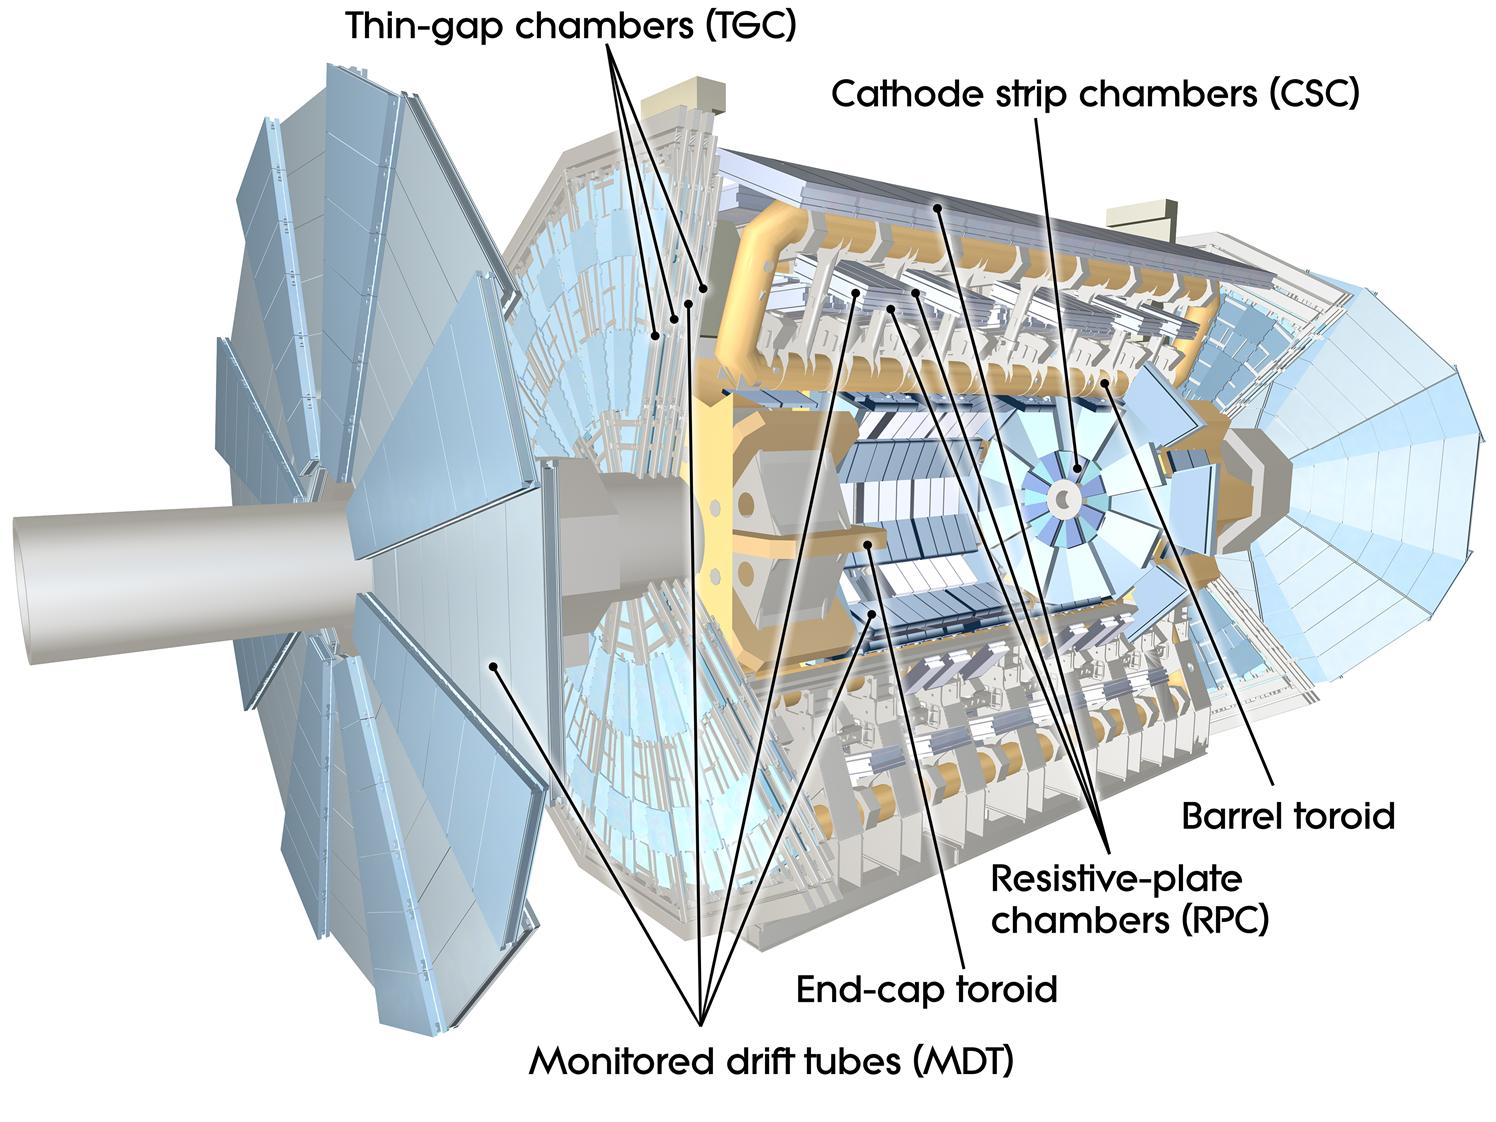
\includegraphics[width=\textwidth]{Detector/MS/MS}
				\caption{Cut-away view of the ATLAS muon system~\cite{ATLASJINST}.}
				\label{fig:MS}
			\end{figure}

			The MS is comprised of one large barrel toroid, covering the region $\left| \eta \right | \leq 1.4$, and two end-cap toroids, covering $1.6 < \left| \eta \right| \leq 2.7$ which are employed together to achieve the track-bending effect wanted. The magnitude of the magnetic field in the barrel, generated by eight large superconducting coils, ranges from 0.5 to 2 T. 

			Around the beam axis, three cylindrical layers make way for the chambers, placed in planes perpendicular to the beam, used to measure tracks. 

			Monitored Drift Chambers (MDTs) are employed over most of the pseudorapidity range to provide precision measurement of track coordinates in the bending direction. 
			Cathode Strip Chambers (CSCs) are instead employed at large pseudorapidity ($2 < \left | \eta \right | < 2.7$). 
			Finally, in the end-cap regions Thin-Gap Chambers (TGCs) together with Resistive-Plate Chambers (RPCs) are dedicated to the Trigger System discussed in Section~\ref{sec:trigSyst}. 


	% --------------------------------
	% -------  THE TRIGGER
	% --------------------------------
	\section{The ATLAS Trigger System}
	\label{sec:trigSyst}

		\begin{figure}[!htb]
			\centering
			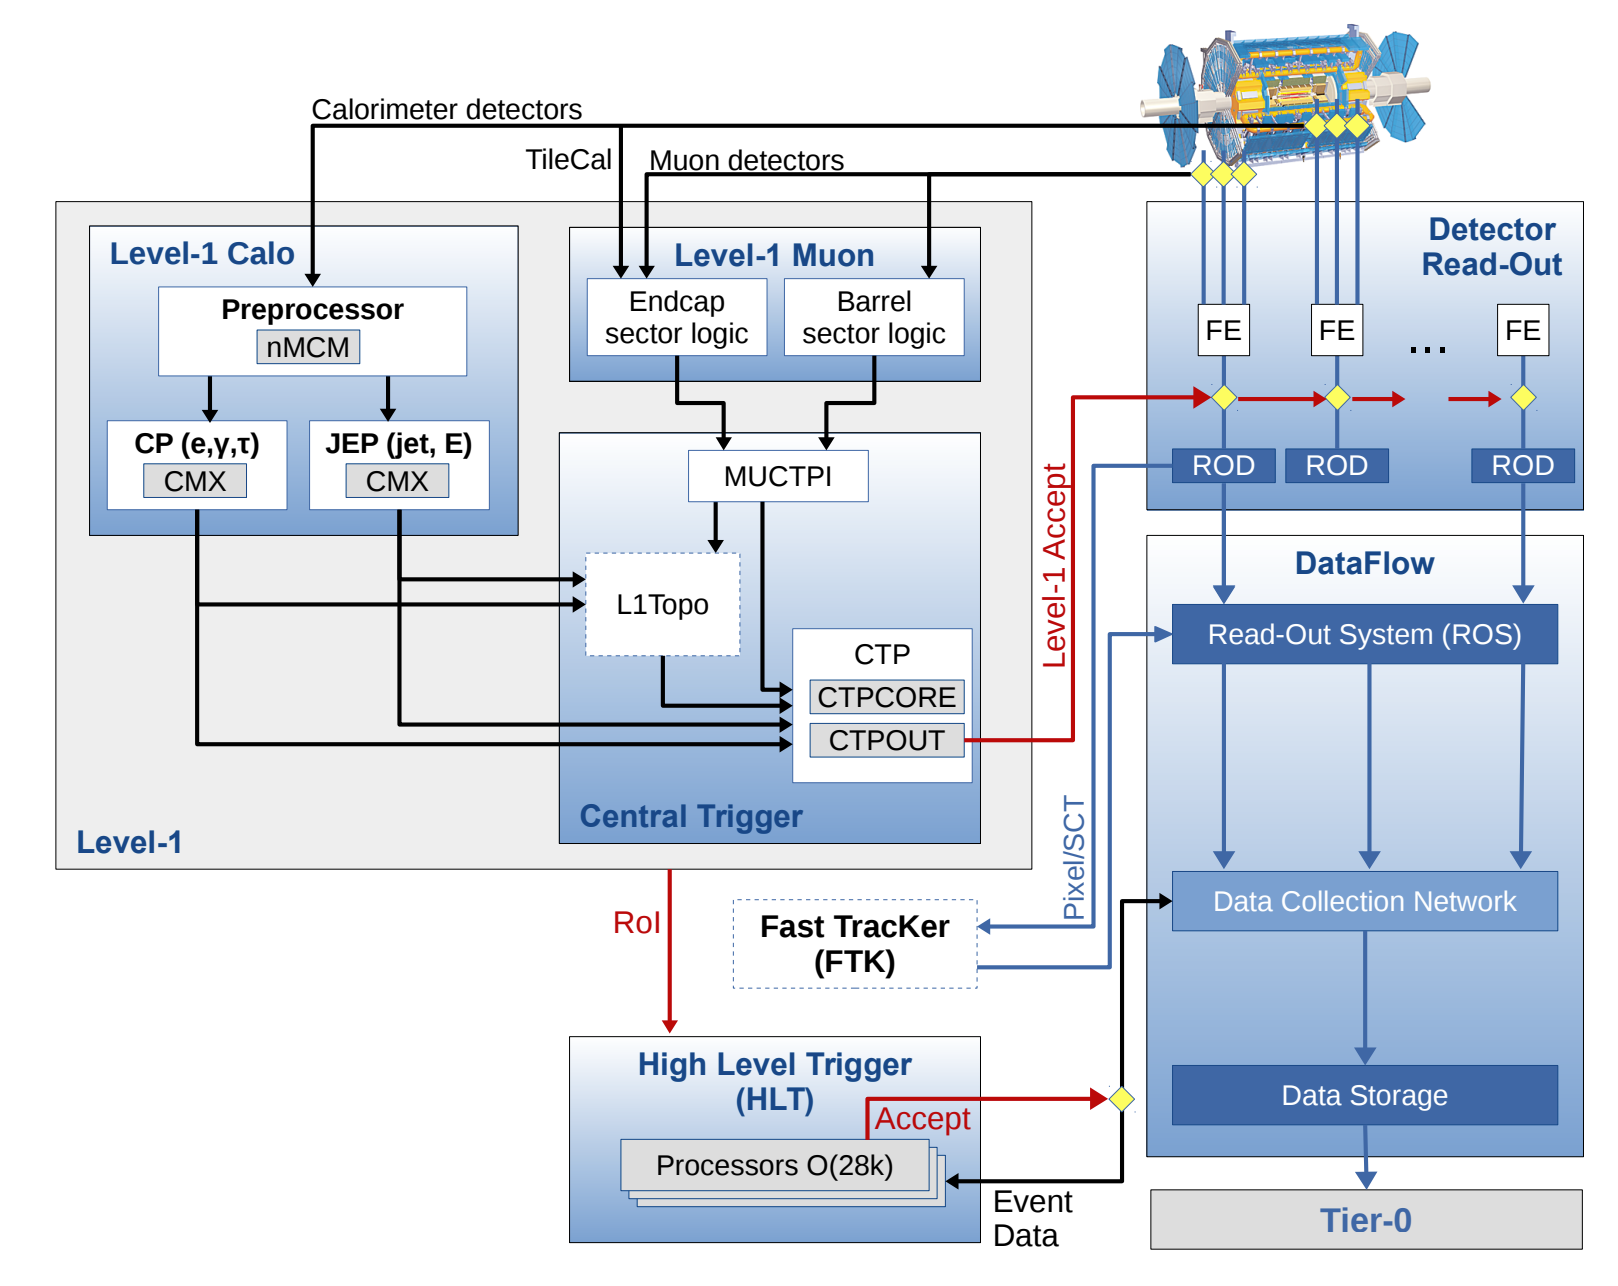
\includegraphics[width=\textwidth]{Detector/Trigger/TDAQSystem}
			\caption{The ATLAS TDAQ system. L1Topo and FTK were being commissioned during 2015 and not used for the results shown in this thesis~\cite{ATLASTrigger2015}.}
			\label{fig:TDAQSyst}
		\end{figure}

		The ATLAS Trigger System is at the heart of data taking. It is an essential component of any nuclear or particle physics experiment since it is responsible for deciding whether or not to store an event for later study~\cite{ATLASTrigger2015}. The ATLAS Trigger system is employed to reduce the event rate from $\sim$ 40 MHz\footnote{The LHC delivers beams with a bunch-spacing of 25 ns.} bunch-crossing\footnote{The term bunch-crossing is hereby used when referring to a collision between two bunches of protons. Since only a certain fraction of the total momentum carried by each proton contributes to the collision, an average number of interactions per bunch-crossing, $\left < \mu \right >$ is used.} to $\sim$ 200 Hz which corresponds to roughly 300 MB/s.

		The Trigger and Data Acquisition (TDAQ) system shown in Figure~\ref{fig:TDAQSyst} consists of a hardware-based first level trigger (L1) and a software-based high-level trigger (HLT). The L1 trigger decision is formed by the Central Trigger Processor (CTP), which receives inputs from the L1 calorimeter (L1Calo) and L1 muon (L1Muon) triggers. The first level (L1), which was designed to perform the first selection step, is a hardware-based system that uses information from the calorimeter and muon subdetectors. It also defines the so-called Regions of Interest (RoIs) within the detector to be investigated by the next level trigger, the HLT. Additionally, a Fast TracKer (FTK) system~\cite{FTKTDR} (not yet installed) will provide global ID track reconstruction at the L1 trigger rate using lookup tables stored in custom associative memory chips for the pattern recognition. The FPGA-based track fitter will perform a fast linear fit and the tracks are made available to the HLT. This system will allow the use of tracks at much higher event rates in the HLT than is currently affordable using CPU systems. However, the upgrade of the ATLAS trigger will not be discussed any further.

		In the next sections the L1 and HLT will be briefly described. 


		\subsection{Level 1 Trigger}

			The Level 1 Trigger identifies Regions of Interest (RoIs)\footnote{$\eta - \phi$ regions where event features have been fouind by the L1 selection process.} and passes these to HLT which will perform further investigations. Furthermore, in order to decide whether or not the event processing will continue, L1 selection uses only information coming from some parts of the detector to keep the input rate to a maximum of 100 kHz. L1 is implemented in fast custom electronics to keep the latency\footnote{Time needed by an electric signal to get to the front-end electronics.} below $2.5\, \mu$s. Event data from other sub-sytstem are temporarily stored in memories whilst L1 decision is taken. 

			The L1 topological trigger (L1-Topo)~\cite{ATLASL1Topo} is feeded with energy and direction information, about the objects found by the L1 calorimeter and the muon trigger, which will be processed by dedicated algorithms implemented in its own FPGAs. However, due to the 100 kHz read-out rate, not all the information collected by L1-Topo will be sent to the HLT, but only part of it. In order to properly seed the RoI-guided HLT reconstruction, speficic objects in combination with the correct topological criteria must be employed.


		\subsection{High-Level Trigger}

			The HLT is used to reduce the output rate down to 1 kHz and it has a $\sim$200 ms average decision time. Events that pass L1 trigger are then processed by the HLT using finer-granularity calorimeter information, precision measurements from the MS and tracking information from the ID. The HLT reconstruction can be run within RoIs identified at L1 or a so-called full-scan on the full detector can be performed. The track reconstruction in the Inner Detector is an essential component of the trigger decision in the HLT and it will be discussed more in detail in Chapter~\ref{ch:trigger}








        \chapter{The ATLAS Trigger System}
\label{ch:trigger}

	The ATLAS trigger system together with its performance will be presented in this chapter. A brief introduction, about the reason behind the need of a trigger system together with its implementation in ATLAS will be discussed in Section~\ref{sec:Trig_intro}. The algorithms used for the tracking in the inner detector will then be described in Section~\ref{sec:tracking}. Ultimately, measurements of the performance of the low transverse momentum single lepton triggers and medium and high trasnverse momentum \bj\ triggers, as part of the \textit{qualification task}\footnote{In order to become an ATLAS author, a person must have been an active ATLAS member for at least one year working on a technical work} of the author, will be discussed in Section~\ref{sec:Trig_perf}. 



	\section{Overview}
	\label{sec:Trig_intro}

		In 2016 and 2017 LHC performed incredibly well delivering more than 80 \ifb\ of \pp\ collisions. As previously mentioned in Section~\ref{sec:trigSyst}, due to storage space limitations it is not feasible to save all the information about the collision after every bunch crossing, so the ATLAS Trigger System is indispensable to reduce the read-out rate to a sensible value without affecting the physics programme of ATLAS, \eg\ discarding potentially interesting events. A multiple-level architecture is employed to allow the trigger some more time such that the identification, of an interesting event, using both software- and hardware-based real-time algorithms to determine whether or not a bunch-crossing contains interesting physics, is made possible. 

		\begin{figure}[!htb]
			\centering
			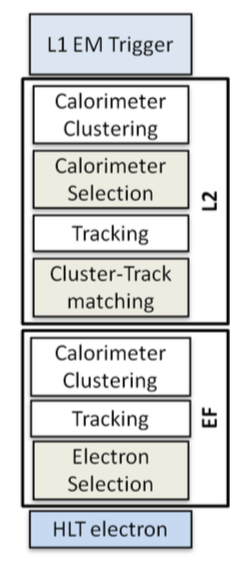
\includegraphics[height=.3\textheight]{Trigger/trig_chain}
			\caption{\label{fig:trig_chain} An Electron-trigger chain (from \cite{ATLASTrigger2010}).}
		\end{figure}

		The trigger system is configured via the so-called trigger \textit{menu} that is meant to define the trigger \textit{chains} - usually referred to just as trigger - that start from a L1 trigger and specify a sequence of reconstruction and selection steps for the specific trigger signatures required in the trigger chain. Fig.~\ref{fig:trig_chain} shows an illustration of an electron-trigger chain used to select electrons \cite{ATLASTrigger2010}.

		The two levels will be discussed in the following sections.


		
		\subsection{Level 1 Trigger}
		\label{sec:L1}

			The Level 1 (L1) trigger decision is formed by the Central Trigger Processor (CTP), based on information from the calorimeter trigger towers and dedicated triggering layers in the muon system. The CTP forms the L1 trigger decision by applying the multiplicity requirements and prescale factors specified in the trigger menu to the inputs from the L1 trigger systems. The CTP also provides random triggers and can apply specific LHC bunch crossing requirements. The L1 trigger decision is distributed, together with timing and control sig- nals, to all ATLAS sub-detector readout systems.

			The first level, known as Level 1 (L1) trigger, is a hardware-based stage. It processes low-granularity information from the calorimeter and the muon spectrometer and identifies the so-called Regions of Interest (RoIs)\footnote{$\eta - \phi$ regions where event features have been found by the L1 selection process.} before making a decision. It then feeds the next level, the high-level trigger (HLT) which will perform further investigations. L1 is implemented in fast custom electronics to keep the decision time around 2.5 $\mu$s. Event data from other sub-sytstem are temporarily stored in memories whilst L1 decision is taken. 			

			During the long shutdown (LS1), various upgraded were implemented in order to prepare for the expected higher rates in Run 2. A new topological trigger (L1-Topo) consisting of two FPGA-based (Field-Programmable Gate Arrays) processor modules was added in L1. L1-Topo~\cite{ATLASL1Topo} is fed with energy and direction information, about the objects found by the L1 calorimeter and the muon trigger, which will be processed by dedicated algorithms implemented in its own FPGAs. However, due to the 100 kHz read-out rate, not all the information collected by L1-Topo will be sent to the HLT. In order to properly seed the RoI-guided HLT reconstruction, speficic objects in combination with the correct topological criteria must be employed.




		\subsection{High-Level Trigger}
		\label{sec:HLT}

		%BEN's

		% The rest of the trigger is made up of software running on a commercially available computer cluster and is known as the high level trigger (HLT). In Run 1 the HLT was split into two levels: the level 2 (L2) and event filter (EF) triggers. The L2 was custom written software which processed data at the full detector granularity within the RoIs from L1. It performed calorimeter reconstruction, the earliest available Fast Tracking, and track-cluster matching. It had a peak output of about 6.5 kHz with an average decision time of about 75 ms. The EF was an optimised version of the standard ATLAS reconstruction software which can run on the full granularity data from the entire detector. It performed the full reconstruction and precision tracking to make the final event selection. It had a peak output rate of about 700 Hz with an average decision time of about 1 s. Each of these stages ran separately with a new node in the computer cluster being assigned to the event between the L2 accepting the event and the event filter making a decision on the event.

		% In Run 2 the HLT has been merged into a single process running on a single HLT computing cluster node. This simplifies the data-flow removing the need for network communication between the L2 and EF triggers and removes the duplication in requesting data from the DAQ system. It also means the EF trigger doesn’t have to first perform event building after the L2 accept as the event building can flexibly be placed as a step during the processing of the algorithms on the single HLT CPU node. The new combined trigger has a peak output rate of about 1 kHz and an average decision time of about 200 ms. A new hardware-based track preprocessor known as the Fast TracKer (FTK) [35] is planned to be added in Run 2. It will process events after the L1 trigger accept in order to seed the HLT algorithms.


			The HLT is used to reduce the output rate down to 1 kHz and it has a $\sim$200 ms average decision time. Events that pass L1 trigger are then processed by the HLT using finer-granularity calorimeter information, precision measurements from the MS and tracking information from the ID. The HLT reconstruction can be run within RoIs identified at L1 or a so-called full-scan on the full detector can be performed. The track reconstruction in the Inner Detector is an essential component of the trigger decision in the HLT and it will be discussed more in detail in Chapter~\ref{ch:trigger}




	\section{The tracking}
	\label{sec:tracking}



	\section{Performance of HLT}
	\label{sec:Trig_perf}

		\subsection{Electrons}

		\subsection{Muons}

		\subsection{$b$-jets}


        \chapter[Event Simulation and Object Reconstruction]{Event Simulation and \protect\\Object Reconstruction}
\label{ch:evSimObjReco}
\epigraph{\emph{Nature isn't classical, dammit, and if you want to make a simulation of nature, you'd better make it quantum mechanical, and by golly it's a wonderful problem, because it doesn't look so easy.}} {Richard P. Feynman}

	The \ac{ATLAS} software framework Athena~\cite{TDR2005}, which is based on the Gaudi~\cite{Gaudi2000} framework developed by \ac{LHCb}~\cite{LHCb2008}, is used to reconstruct physics objects to be used by analysers, as the data collected and recorded by the \ac{ATLAS} detector requires processing. The Athena framework is capable of dealing with various aspects of the experiment software, \eg\ triggering or the processing of simulated data. Custom softwares, in particular \ac{MC} simulations, are used to simulate physics events used to model background and signal process. These are produced through different stages, as shown in Figure~\ref{fig:workflow}, the last of which produces an output with an analyser-friendly format. 

	In this chapter the stages will be briefly explained as it follows: Event Generation (Section~\ref{sec:evGen}) and the Detector Simulation (Section~\ref{subsec:detSim}). The reconstruction of physics objects\footnote{A set of criteria needs to be applied in order to reconstruct the detected object as an ``electron'', ``photon'', ``muon'', ``jet'', etc.}, in both collected data and simulated \ac{MC} events, will be described in Section~\ref{sec:objReco}. Finally, a set of selection criteria are applied to reconstructed objects to identify those suitable for use in analysis, as detailed in Section~\ref{sec:objSel}.

	\begin{figure}
		\centering
		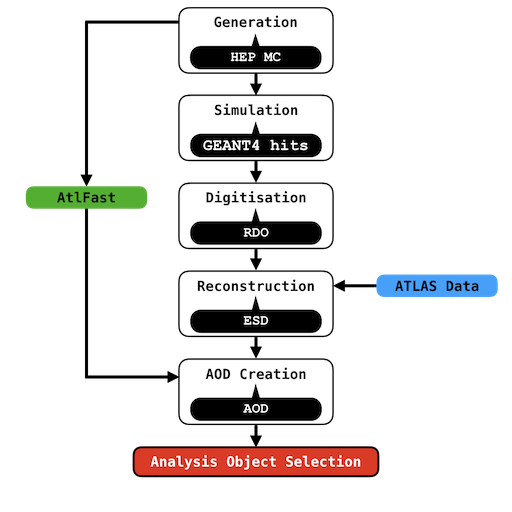
\includegraphics[width=.75\textwidth]{MCobj/flow}
		\caption{\label{fig:workflow} Illustration of the different stages of the workflow needed to produce analysable simulated and collected data outputs. The white boxes represent the processes, and their outputs are shown in black balloons: \ac{RDO}, \ac{ESD}, and the final product, \ac{AOD}. The green `AtlFast' box represents the alternative simulation method \textsc{Atlfast}~\cite{Lukas2012}, discussed in Section~\ref{subsec:detSim}. Finally, the blue box shows the stage at which the actual \ac{ATLAS} data events begin processings.}
	\end{figure}



	\section{Generation of a MC-simulated event}
	\label{sec:evGen}

		\ac{MC} event generators~\cite{Buckley:2011ms} are extensively used in particle physics to simulate \ac{SM} and \ac{BSM} physics processes. A combination of perturbative and phenomenological calculations, to produce randomly distributed physics events, of a given type, with stable final state particles, is employed. As already mentioned in Chapter~\ref{ch:detector}, The \ac{ATLAS} detector collects \pp- and heavy-ion-collisions data. When two protons collide at such high energy in the center of mass, the collision essentially occurs between the nucleon constituents: partons\footnote{``\emph{Feynman~\cite{PhysRevLett.23.1415} interpreted the Bjorken scaling as the point-like nature of the nucleon's constituents when they were incoherently scattered by the incident electron. Feynman named the point-like constituents partons. This is the parton model.}''(taken from~\cite{Yan:2014kna})}. Three valence quarks (uud), the gluons mediating the strong interactions between the valence quarks, and the sea quarks produced in virtual \qqbar\ pairs due to interacting gluons, are included in the partons. Figure~\ref{fig:DIS} shows one of these interactions which are known as \ac{DIS} processes, simply because the substructure of the proton is probed, therefore \emph{deep}, by an incoming particle, in this case a proton, whose momentum is not conserved in the process, therefore \emph{inelastic}.

		\begin{figure}[!htb]
			\centering
			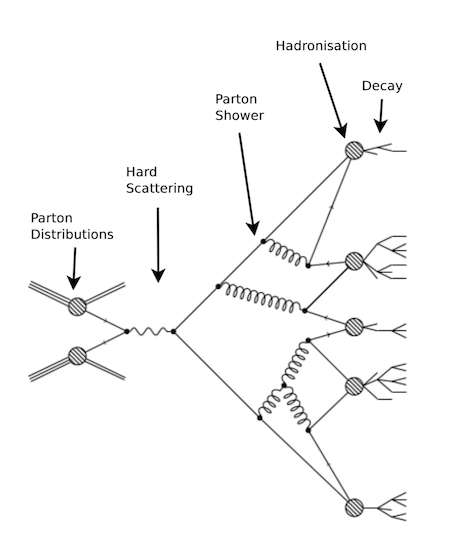
\includegraphics[width=.5\textwidth]{MCobj/ppcollision}
			\caption{\label{fig:DIS} Example of a \pp\ \ac{DIS} event.}
		\end{figure}

		An important yet simplifying dimensionless physical quantity is the Bjorken scaling~\cite{PhysRev.179.1547}, which represents the fraction, $x$, of the proton momentum carried by an interacting parton. The measure of momentum transfer, $Q^2$, in such events, is related to the momentum transferred by the exchanged boson, $q$, by $Q^2 = -q^2$. \ac{PDFs} are used to describe mathematically the parton content of the colliding protons in order to model their interaction.  

		The \pp\ scattering at the \ac{LHC} can be categorised in processes such as \emph{hard}, which can be described with perturbation theory, or \emph{soft}, which involve non-perturbative \ac{QCD} effects. Tipically, a \pp\ collision involves a hard scattering process between two partons, one for each proton, and a certain number of soft processes, such as \ac{ISR}, \ac{FSR}, and \ac{UE}. The \ac{ISR} involves particles, that are radiated by partons, which will interact in the hard process prior to their scattering. Those partons, which are not involved in the hard scattering process, the so-called \emph{spectators}, form the \ac{UE}. The \ac{FSR} refers to particles that are radiated from the final state products of the hard scattering. Furthermore, \emph{parton showering} is a process in which particles in the event that have colour can radiate gluons and/or produce \qqbar\ pairs. Products of these showers will undergo the process of \emph{hadronisation} during which colourless hadron states are produced if $Q^2$ is of the order of $1 \GeV$. Such a process occurs due to confinement. 

		%The modelling of the hard process, parton showering and hadronisation within the event, will be briefly described in Sections~\ref{sec:ME},~\ref{sec:PS} and~\ref{sec:hadronisation}. Section~\ref{sec:UE} describes how to model of the UE. 
		In order to allow analysers to select samples with relevant processes, \ac{MC} samples are divided in categories depending upon the hard-process specified before generation. It is also possible to filter events to only produce a given final state, \eg\ asking for zero leptons, in order not to waste computational resources on events which would not pass any selection criteria, regardless, improving the available statistics. The effect of the selection will be taken into account by applying filter efficiency when the analysis is carried out. The \textsc{HepMC} format is used to store the output of simulated data outputs~\cite{DOBBS200141}.

			\paragraph*{Parton Distribution Function}
			%\label{sec:pdf}

				\ac{PDFs}~\cite{Campbell2007} mathematically describe the probability density of constituent partons of the interacting protons to have a fraction, $x$, of the nucleon momentum. They depend upon the parton type such as, valence quark, gluon, or sea quark, and the momentum transfer $Q^2$. Although perturbative calculations of the \ac{PDFs} are not feasible, the \textsc{DGLAP}~\cite{Gribov:1972ri, Altarelli:1977zs} evolution equations, using a range of hard scattering data from both fixed target and collider experiments, can be used to estimate the dependance as a function of $Q^2$ for a given parton. In other words, \ac{PDFs} describe the evolution of the structure functions of quarks and gluons as a function of the running\footnote{Referred to a dependence on $Q^2$} strong coupling constant $\alpha_s$. Figure~\ref{fig:HERAPDF} shows the \ac{PDFs}, calculated with input from \textsc{HERA} and \textsc{CTEQ} at $Q^2 = 10 \GeV^2$ for up and down valence quarks, gluons, and sea-quarks.

				\begin{figure}[!htb]
					\centering
					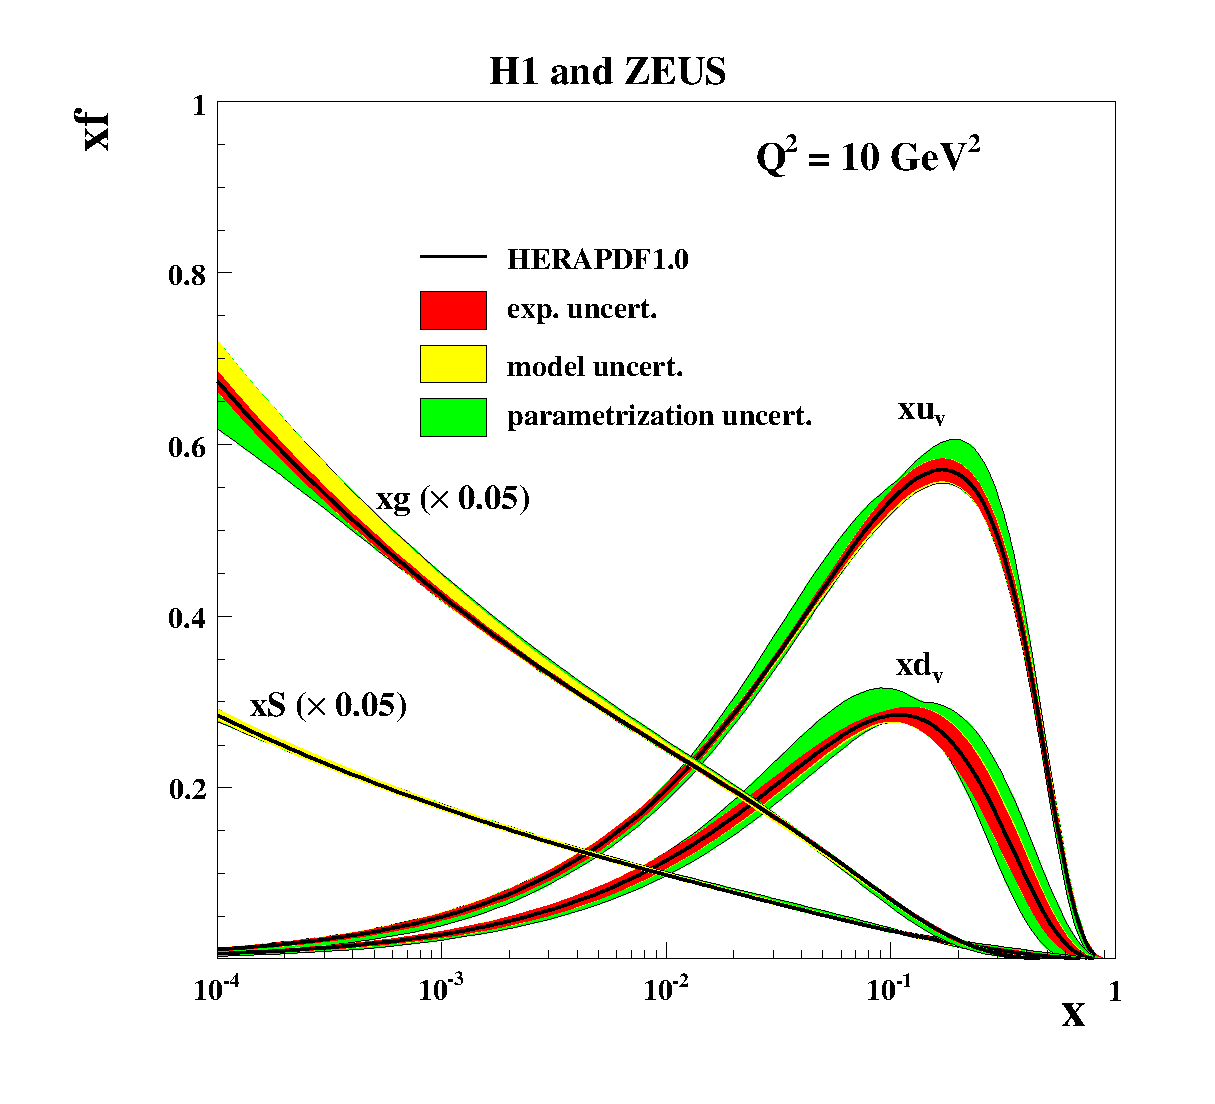
\includegraphics[width=.5\textwidth]{MCobj/d09-158f18b}
					\caption{\label{fig:HERAPDF} PDF from \textsc{HERAPDF1.0}, for up and down valence quarks $xu_v$ and $xd_v$ , gluons $xg$, and sea quarks $xS = 2x(\bar{U} + \bar{D})$, using a momentum transfer of $Q^2 =10 \GeV^2$ (from~\cite{Aaron:2009aa}).}
				\end{figure}

			\paragraph*{Matrix Element}
			%\label{sec:ME}

				The matrix element is a simulation stage used to compute the hard processes, where a large momentum transfer ($Q^2 > \mathcal{O}(1 \GeV)$) is involved, which can be calculated using quantum field theory techniques. Matrix elements to \ac{LO} or \ac{NLO} in an expansion in $\alpha_s$, to calculate a probabilistic distribution of the outgoing partons, are used to make \ac{PDFs} simulate partons coming into the hard scatter process. Hard emissions, namely the production of high momentum quarks and gluons in the event, therefore procceses such as, a gluon splitting into two gluons, $g \to gg$, or a gluon decaying to a quark-antiquark pair $g \to \qqbar$, and a quark radiating a gluon ($q \to gq$), can be added into the matrix element.

			\paragraph*{Parton Showers}
			%\label{sec:PS}

				The emission of extra soft objects cannot be modelled with the matrix element, due to its non-perturbative nature. \ac{PS} generators are instead used to include processes such as the emission of a gluon by a quark ($q \to qg$), or the emission of \qqbar\ pairs $g \to qq$ or a gluon pair by a gluon $g \to gg$. \textsc{Herwig}~\cite{Herwig2001}, \textsc{Pythia}~\cite{Pythia2006}, and \textsc{Sherpa}~\cite{Sherpa} collaborations have developed the most used \ac{PS} models across the \ac{ATLAS} community and beyond. Markov chains~\cite{Berg2004} are the heart of the algorithms used to simulate \ac{PS}. These use probabilities that a gluon is radiated or a \qqbar\ pair is produced. %The decision of whether or not these processes will occur is made at each point in the chain. 

				At intermediate $Q^2$, gluon/quark radiation may be treated as a hard emission or part of the \ac{PS}, meaning that, in a given event double-counting might occur. To overcome such issue, the \ac{CKKW}~\cite{QCD2001}, and the \ac{MLM}~\cite{ME2001}, schemes are employed to determine whether the emissions are part of the matrix element or \ac{PS}. As the energy of the partons decrease below $1 \GeV$ they will undergo hadronisation.

			\paragraph*{Hadronisation}
			%\label{sec:hadronisation}

				As previously mentioned in Section~\ref{sec:SMov}, once the quarks and gluons in the final state reach a $Q^2$ of the order of $\Lambda_{\mathrm{QCD}} \sim 200 \MeV$, the recombination into colourless objects must occur. The modelling of the production of such bound state, the hadronisation, involves non-perturbative \ac{QCD} and many more parameters than the parton showering. Phenomenological models, tuned using data, are then needed. The cluster model~\cite{ClusterHerwig1999}, used by \textsc{Herwig}, and the Lund string model~\cite{LundModel2002}, used by \textsc{Pythia}, are the most employed. 

			\paragraph*{Underlying Event}
			%\label{sec:UE}

				Partons not involved in the hard process of the event, referred to as the \ac{UE}~\cite{Field2008}, can lead to a certain number of soft interactions at a lower energy scale, therefore producing additional hadronic activity in the event. Once again, phenomenological models are used to account for such effect which is modelled within \textsc{Sherpa} and \textsc{Pythia} where a whole lot of additional free tuned-to-data parameters are included. More details can be found in~\cite{Field2008}.



		\subsection{Detector simulation}
		\label{subsec:detSim}

			Although at this stage the output of the \ac{MC} generators contains all the kinematic features of the event, it is not yet possible to compare to the \ac{ATLAS} collected data, as the interactions of the particles passing through the detectors are not yet included. The \textsc{Geant4} software~\cite{Geant42003}, included within the \ac{ATLAS} offline software\footnote{All the software made available for analysers to be used after the data have been collected}, is used to simulate the energy deposited within the detector: a first stage is run to simulate the interactions of the particles with the various sub-systems, and a second one is run to convert energy deposits into detector-output-like signals (voltage, times, etc.). This is the so-called \emph{digitisation}. The ouput is now produced with a format that is identical to the one produced by the \ac{ATLAS} \ac{TDAQ} system, therefore \ac{MC} and collected \ac{ATLAS} data can now be consistently processed by the same trigger and reconstruction softwares. Nonetheless, the \ac{ATLAS} Collaboration also use faster simulation software such as \textsc{Atlfast-II} (AF2)~\cite{Lukas2012} where, in order to reduce the usage of the available computational resources, a parametrised description of the showers in the calorimeters is implemented. 


	\section{Object Reconstruction}
	\label{sec:objReco}

		At this stage both \ac{MC} and data samples contain all the electronic pulses from the digitisation process. These have to be turned into tracks and calorimeter deposits which, in turn, have to processed to be reconstructed into physics object, such as electrons, photons, muons, jets, taus, and missing energy, \met. Initally, a set of loose definitions is employed in order for various analyses to use such objects. Later, a set of tighter cuts can be applied depending on what a particular analysis needs to focus on. This approach increases the purity of the selected objects at the expense of selection efficiency. The criteria used to define the physics objects, relevant to the analysis presented in this thesis, will be presented in the following paragraphs.


		\paragraph*{Tracks and vertices}

			When a charged particle passes through the detector, all the \ac{ID} sub-systems, pixel, \ac{SCT} and \ac{TRT} components, register ``hits''and then, tracing the particle's trajectory, the hits are reconstructed into a ``track''. The most used algorithm is the so-called \emph{inside-out} method, whose clue is in the name: it works outwards from the center of the \ac{ID} to produce a track once it has initially grouped together hits in the pixel and \ac{SCT} sub-systems. If this track is then compatible with hits in the \ac{TRT} detector, then these hits are also included and the track is accepted. The back-tracking algorithm uses the same approach, but in the opposite order, working from the \ac{TRT} to the \ac{SCT} and Pixel detectors, and tracks can also be reconstructed using only the hits in the \ac{TRT}. 

			% The ID tracks are then matched up with candidates for charged particles produced from signals in other parts of the detector, for example the ECAL cluster for an electron. A number of selection cuts are made on the tracks before this stage to ensure that they are of the required quality. The tracks are assigned values of η and φ using their direction with respect to the origin in the right-handed co-ordinate system described in Section 3.3. The origin is taken to be the position of the primary interaction, as discussed in Section 4.1. In addition, d0 is defined as the distance of closest approach between the track and the origin, and z0 is defined as the z-plane component of d0. The parameter z0 sin θ gives the projection of d0 onto the z-axis, and is also used. The transverse momentum pT of a track is related to the magnetic field B, and the bending radius R, which quantifies the bending of the track trajectory due to B. The relationship is given as pT (GeV)= 0.3×B (T)×R (m). The following cuts are applied to all tracks referred to after this point, unless otherwise specified:


		\paragraph*{Electrons}

		\paragraph*{Muons}

		\paragraph*{Photons}

		\paragraph*{Jets}

		\paragraph*{Missing Transverse Energy}

			 



	\section{Object Selection}
	\label{sec:objSel}

		\subsection{Baseline Object Selection}
		\label{subsec:baseObjSel}

			\paragraph*{Leptons}
			
			\paragraph*{Photons}
			
			\paragraph*{Jets}


		\subsection{Overlap Removal}
		\label{subsec:OR}

		\subsection{Signal Object Selection}
		\label{subsec:sigObjSel}

			\paragraph*{Leptons}

			\paragraph*{Photons}

			\paragraph*{Jets}
        \chapter[Search for top squarks in all-hadronic final states]{Search for top squarks \protect\\in all-hadronic final states}
\label{ch:stop_ana}
\epigraph{\emph{In God we trust. All others must bring data.}}{W. Edwards Deming}

	In this chapter the core of this thesis will be presented, namely the search for the direct pair-production of the supersymmetric partner of the top quark in all-hadronic final states using $36.1\, \ifb$ of \pp\ collisions, at a centre-of-mass energy $\rts = 13$ \TeV, delivered by the \ac{LHC} and collected by the \ac{ATLAS} detector~\cite{stop0L}. 

	\section{Overview}



	% \section{Object Selection}
	% \label{sec:objSel}

	% 	\subsection{Baseline Object Selection}
	% 	\label{subsec:baseObjSel}

	% 		\subsection*{Leptons}
			
	% 		\subsection*{Photons}
			
	% 		\subsection*{Jets}


	% 	\subsection{Overlap Removal}
	% 	\label{subsec:OR}

	% 	\subsection{Signal Object Selection}
	% 	\label{subsec:sigObjSel}

	% 		\subsection*{Leptons}

	% 		\subsection*{Photons}

	% 		\subsection*{Jets}
        % \chapter{Results and statistical interpretation}
\label{ch:results}
\epigraph{\emph{In God we trust. All others must bring data.}}{William E. Deming}

	The results of this analysis were published in a paper in the Journal of High Energy Physics in September 2017~\cite{stop0L}. A previous version of the analysis was also made public, using $13.3\,\ifb$ collected at $\rts = 13$ \TeV, with an earlier subset of the whole $2015+2016$ dataset, documented in an ATLAS conference note~\cite{ICHEPstop0L}. Although both versions contain the author's contribution on the optimisation of the \acp{SR} and the estimation of the irreducible background $\ttZ (\to \nu\nu)$, only the results of the most recent analysis will be hereby discussed, as it represents the most updated, improved and extended version. The chapter is structured as it follows: Section~\ref{sec:stat_ana} is dedicated to a brief overview of the statistical analysis and the tools employed; the results together with their interpretations will be shown in Section~\ref{sec:results}. In addition, the results of the background estimation procedure, previously presented in Chapter~\ref{ch:bkgest}, will be shown in Appendix~\ref{app:ttzdm} for an interpretation of the results in terms of production of a Dark Matter candidate in association with third-generation quarks.


	\section{Statistical analysis}
	\label{sec:stat_ana}

		Although a basic estimate of the value of the relevant parameters in signal and control regions can be obtained by solving systems as the one in Equation~\ref{eq:mu_factors}, a statistical tool, that takes into account all the uncertainties (statistical and systematic), is needed to produce quantitative results. The statistical tool - widely used in the ATLAS SUSY working group - to produce the analysis results is the \texttt{HistFitter} framework~\cite{histfitter}. In particular, such framework is used for the implementation of two procedures: parameter estimation, such as \ac{SM} background normalisation factors in Equation~\ref{eq:mu_factors}, and hypothesis test, which allows to measure the parameters from a given dataset, and to check the compatibility of the results obtained from the data analysis with a given hypothesis. \texttt{HistFitter} uses a frequentist approach, where an event's probability is defined as the limit of its relative frequency in a large number of trials.

		\subsection{Estimation of the parameters and the statistical hypothesis testing}

			The interpretation of the data in control, validation, and signal regions needs the estimation of the \ac{SM} background normalisation factors, $\mu_\mathrm{b}$, and the signal strength, $\mu_\mathrm{s}$. Given a set of selection cuts, the expected number of events in a region $R$ $\left ( N_{\mathrm{R}} \right )$ can be calculated as: 

			\begin{equation}
				N_{\mathrm{R}} = \mu_\mathrm{s} N_{\mathrm{s}} + \sum_i \mu_\mathrm{b}^i N_{\mathrm{b}}^i
			\label{eq:nevt_regionR}
			\end{equation}

			\noindent Here, $N_{\mathrm{b}}^i$ and $N_{\mathrm{s}}$ are the expected \ac{MC} yields for the $i^{\mathrm{th}}$ background and the signal, respectively. Taking into account all the systematic uncertainties, a set of so-called \emph{nuisance parameters}, describing how signal and background are affected by the uncertainties, can be introduced and Equation~\ref{eq:nevt_regionR} will be modified as it follows:

			\begin{equation} 
				N_{\mathrm{R}} = \mu_\mathrm{s} N_{\mathrm{s}} \left ( 1 + \sum_j \theta_\mathrm{s}^j \sigma_\mathrm{s}^j \right ) + \sum_i \mu_\mathrm{b}^i N_{\mathrm{b}}^i \left ( 1 + \sum_j \theta_\mathrm{b}^{ij} \sigma_\mathrm{b}^{ij} \right )
			\label{eq:nevt_regionR_nuisance}
			\end{equation} 

			\noindent $\theta_\mathrm{s}^j$ is the $j^{\mathrm{th}}$ nuisance parameter. The numbers $\sigma_\mathrm{s}^j$ and $\sigma_\mathrm{b}^{ij}$ are the signal and backgrounds yields after taking into account the effect of the systematics. Equation~\ref{eq:nevt_regionR_nuisance} is built to reflect a $\pm 1 \sigma$ variation due to the systematic error $\sigma$ when $\theta = \pm 1$, and to return the nominal (non varied) yields when $\theta = 0$. %Nuisance parameters can be either applied to multiple processes if they are common to them, \eg\ \ac{JES}, or they can be applied to a single process, \eg\ theory uncertainties.

			A likelihood function, $L$, containing all the relevant parameters and information from the analysis, allows the extraction of the \ac{SM} background normalisation factors, $\mu_\mathrm{b}$, signal strength, $\mu_\mathrm{s}$, and the nuisance parameters $\theta$. The number of observed events in every \ac{SR} or \ac{CR} can be used to constrain the free parameters contained in the likelihood function, of which a general expression is the following:

			\begin{equation}
				\begin{split}
					L \left ( \bm{N}^{\mathrm{obs}}, \bm{\theta^0} | \mu_\mathrm{s}, \bm{\mu_{\mathrm{b}}, \theta} \right ) & = P_{\mathrm{SR}} \times P_{\mathrm{CR}} \times C_{\mathrm{syst}} = \\
					& = \prod_{i \in \mathrm{CR, SR}} P \left ( N_i^{\mathrm{obs}} | N_i \left( \mu_\mathrm{s}, \bm{\mu_{\mathrm{b}}, \theta} \right) \right ) \times C_{\mathrm{syst}}
				\end{split}
				\label{eq:likelihood}
			\end{equation}

			\noindent This is the product of Poisson distributions of event counts $\left ( {N}^{\mathrm{obs}} \right )$ in \acp{SR} or \acp{CR} ($P_{\mathrm{SR}}$, $P_{\mathrm{CR}}$), times a distribution describing the impact of the systematic uncertainties, $C_{\mathrm{syst}}$. The Poisson factors contain the normalisation factors $\mu_\mathrm{s}$, $\bm{\mu_{\mathrm{b}}}$, and the nuisance parameter $\bm{\theta}$ which is introduced to constrain the systematic uncertainty in the fit. $C_{\mathrm{syst}}$ can be generally treated as a unit Gaussian function such that the fitted values of $\theta_i$ are expected to be approximately $0\pm1$, allowing to reproduce the expected size of the systematic uncertainties using Equation~\ref{eq:nevt_regionR_nuisance}. Further details can be found in Ref.~\cite{histfitter}. The values of the relevant \ac{SM} background normalisation parameters are then obtained by a \ac{MLE}, once the likelihood in Equation~\ref{eq:likelihood} is constructed. Such procedure is discussed in detail in Ref.~\cite{cowan1998statistical}.

			To determine whether a \ac{BSM} signal is discovered or excluded, a statistical procedure known as \emph{statistical hypothesis testing} is employed~\cite{Cowan2015}. A so-called null hypothesis $H0$, to be tested against an alternative $H1$, is defined. In particular, the discovery test for a \ac{BSM} signal is made by choosing $H0$ and $H1$ as the background-only and the signal-plus-background hypotheses, respectively. On the contrary, if such test returns a negative result, namely no \ac{BSM} signal is found, exclusion limits are set by inverting the procedure. 

			The testing procedure is based on the following: a test statistic $t$, with a probability distribution $f(t)$ is defined together with a function of the observed data that assumes large values if the data are incompatible with the null hypothesis ($H0$). Pseudo-experiments (also known as \emph{toys}) are employed in large number to determine the shape of $f(t)$. In such toys all the values of the physical observables can be randomly generated under the null hypothesis. %, alternatively, using a so-called \emph{asymptotic approximation} given the types of test statistics and the size of the statistical samples~\cite{Cowan:2010js}.

			The null hypothesis ($H0$) is tested through the computation of a $p$-value, which represents the probability of observing a larger incompatibility of the data with the predictions in an infinite number of repetitions of the experiment under the assumption that $H0$ is valid. Once the distribution $f(t)$ is known, the computation of the $p$-value can be carried out as:

			\begin{equation}
				p = \int_{t_{\mu,\mathrm{obs}}}^{\inf} f(t)\,dt
 			\label{eq:pvalue}
			\end{equation}

			\begin{figure}[!htb]
				\centering
					\subbottom[]{
						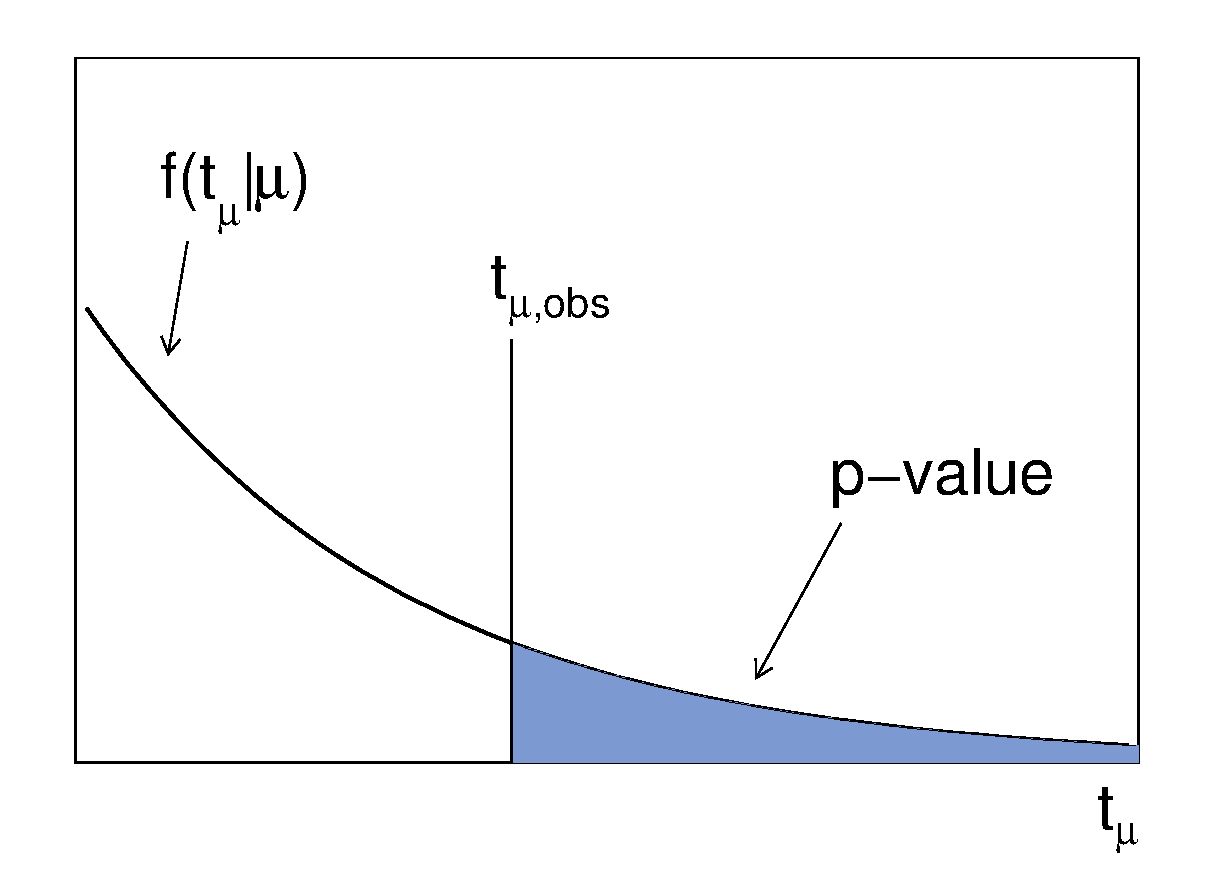
\includegraphics[width=0.45\textwidth]{stop/stat/Pval_tmu}}\hspace{0.05\textwidth}
					\subbottom[]{
						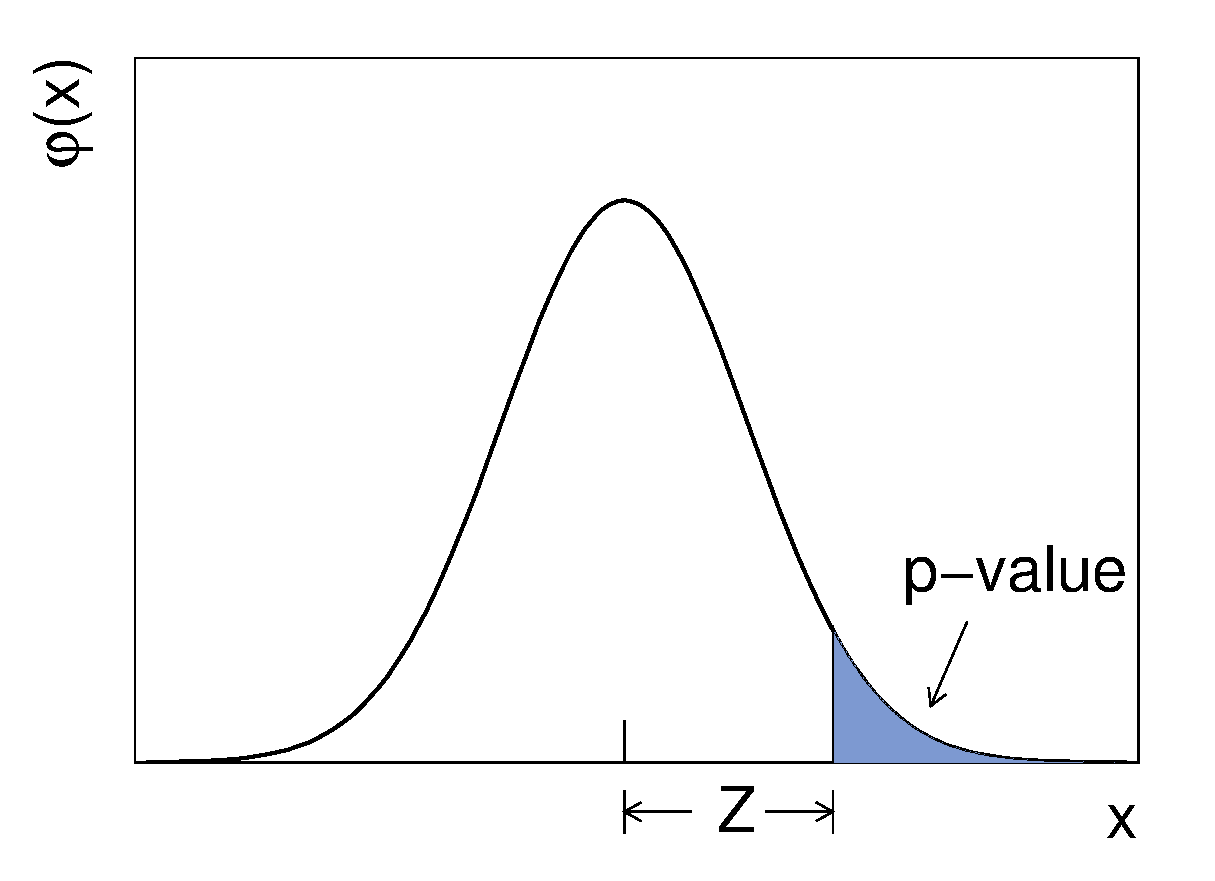
\includegraphics[width=0.45\textwidth]{stop/stat/Significance}}\hspace{0.05\textwidth}
				\caption{Illustration of the relation between the $p$-value obtained from an observed value of the test statistic $t_{\mu}$~(a), and the standard normal distribution showing the relation between the significance $Z$ and the $p$-value (taken from~\cite{Cowan:2010js}).}
				\label{fig:pval-sig}
			\end{figure}

			\noindent where, as shown in Figure~\ref{fig:pval-sig}~(a), $f(t)$ is integrated from the observed value of the test statistic, $t_{\mu,\mathrm{obs}}$, to infinity. As a matter of fact, an equivalent quantity is instead considered, which is equivalent to the $p$-value: the significance, $Z$. For convenience, the $p$-value is converted into the significance, $Z$, defined as the number of standard deviations $\sigma$ from the mean of a Gaussian distribution for which the integral of the tail of the curve is equal to $p$: 

			\begin{equation}
				Z = \Phi^{-1} \left ( 1 - p \right )
			\label{eq:Z_pval}
			\end{equation}

			\noindent Here, $\Phi^{-1}$ is the inverse of the cumulative distribution of the Gaussian, as it can be seen from Figure~\ref{fig:pval-sig}~(b). The particle physics community has chosen $Z = 5$ ($Z=3$) as the minimum value of significance needed to claim a discovery (evidence) against the background-only hypothesis. Such value of significance correspond to a $p$-value of $2.87 \times 10^{-7}$ and $p = 0.0013$, respectively. A significance of $1.64\sigma$ ($p = 0.05$) is instead used to exclude a given signal model.

			The choice of an appropriate test $t$ is an important step in the statistical hypothesis testing procedure. From Equation~\ref{eq:likelihood} a statistic test can be obtained as it follows: 

			\begin{equation}
				\lambda \left ( \mu_{\mathrm{s}} \right ) = \frac{L\left ( \mu_{\mathrm{s}}, \hat{\hat{\bm{\theta}}} \right )}{L\left ( \hat{\mu_{\mathrm{s}}}, \hat{\bm{\theta}} \right )}
			\label{eq:PLR}
			\end{equation}

			\noindent where the vector $\bm{\theta}$ takes into account the background normalisation factors and the nuisance parameters related to the systematic uncertainties. The numerator $L\left ( \mu_{\mathrm{s}}, \hat{\hat{\bm{\theta}}} \right )$ is the maximum for a given value of $\mu_{\mathrm{s}}$, while the denominator $L\left ( \hat{\mu_{\mathrm{s}}}, \hat{\bm{\theta}} \right )$ corresponds to the absolute maximum of the likelihood function. As shown in Equation~\ref{eq:PLR}, $0 < \lambda < 1$: the larger the values the better the agreement of the data with the hypothesis being tested. It is possible to define a test statistic, with the range required by the definition of the $p$-value in Equation~\ref{eq:pvalue}, as $t_{\mu,\mathrm{obs}} = -2 \ln \lambda \left ( \mu \right )$, where the larger the values the lower the compatibility between the observed data and the hypothesis being tested. Two test statistics can be defined, one for discovery and one for exclusion: the former tests the background-only hypothesis and employs a \ac{PLR} function with $\mu_{\mathrm{s}} = 0$; the test can be defined as:
			\begin{align}
			\label{eq:test_discovery}
				\begin{split}
					q_0 & = 
					\begin{cases}
						-2 \ln \lambda \left( 0 \right ) & \hat{\mu_{\mathrm{s}}} \geq 0 \\
						0   & \hat{\mu_{\mathrm{s}}} < 0
					\end{cases}
				\end{split}
			\end{align}
			\noindent The test statistic $q_0$ is set to $0$ for negative $\hat{\mu_{\mathrm{s}}}$ such that the exclusion of the background-only hypothesis, when a deficit of events is observed in the \acp{SR}, can be avoided. The latter, employed for the exclusion of a signal model, employs a test statistic which can be defined as:
			\begin{align}
			\label{eq:test_exclusion}
				\begin{split}
					q_{\mu} & = 
					\begin{cases}
						-2 \ln \lambda \left( \mu_{\mathrm{s}} \right ) & \hat{\mu_{\mathrm{s}}} \leq \mu_{\mathrm{s}} \\
						0   & \hat{\mu_{\mathrm{s}}} > \mu_{\mathrm{s}}
					\end{cases}
				\end{split}
			\end{align}
			\noindent where, the signal strength, $\mu_{\mathrm{s}}$, assumed to be non-zero in the null hypothesis.  

			% \begin{description}
			% 	\item [Discovery:] the background-only hypothesis is tested in this case; a \ac{PLR} function with $\mu_{\mathrm{s}} = 0$ is employed, and it can be defined as:
			% 	\begin{align}
			% 	\label{eq:test_discovery}
			% 		\begin{split}
			% 			q_0 & = 
			% 			\begin{cases}
			% 				-2 \ln \lambda \left( 0 \right ) & \hat{\mu_{\mathrm{s}}} \geq 0 \\
			% 				0   & \hat{\mu_{\mathrm{s}}} < 0
			% 			\end{cases}
			% 		\end{split}
			% 	\end{align}
			% 	\noindent here, $q_0$ is set to $0$ for negative $\hat{\mu_{\mathrm{s}}}$ such that the exclusion of the background-only hypothesis, when a deficit of events is observed in the \acp{SR}, can be avoided.

			% 	\item [Exclusion:] for the exclusion of a signal model, the test statistic can be defined as:
			% 	\begin{align}
			% 	\label{eq:test_exclusion}
			% 		\begin{split}
			% 			q_{\mu} & = 
			% 			\begin{cases}
			% 				-2 \ln \lambda \left( \mu_{\mathrm{s}} \right ) & \hat{\mu_{\mathrm{s}}} \leq \mu_{\mathrm{s}} \\
			% 				0   & \hat{\mu_{\mathrm{s}}} > \mu_{\mathrm{s}}
			% 			\end{cases}
			% 		\end{split}
			% 	\end{align}
			% 	\noindent here, the signal strength, $\mu_{\mathrm{s}}$, assumed to be non-zero in the null hypothesis.  
			% \end{description}

			Unfortunately, for signal models to which the analysis is poorly sensitive, Equation~\ref{eq:test_exclusion} can return a non-negligible probability and, although it can be argued that any constrain on such models should not be put, it is still possible that in the signal-plus-background hypothesis low $p$-values can be obtained when the observed events in the \acp{SR} are fewer than the predicted ones. The introduction of an alternative \acl{FoM} (FoM) for the exclusion can be employed~\cite{Read:2002hq}:

			\begin{equation}
				\mathrm{CL}_s = \frac{p_{\mu_{\mathrm{s}}}} {1 - p_{_\mathrm{b}}}
			\label{eq:cls}
			\end{equation}

			\noindent where $p_{_\mathrm{b}}$ and $p_{\mu_{\mathrm{s}}}$ correspond to the $p$-values of the background-only and signal-plus-background hypotheses, respectively. A $95\%$ \ac{CL} is reached when $\mathrm{CL}_s < 0.05$, \ie\ a threshold of $Z = 2$. Ultimately, when discovery and exclusion test statistics show similar distributions, this will translate into a numerator and denominator of the same order (Equation~\ref{eq:cls}), which guarantees that signals are not excluded, as one would expect.


			\subsection{Discovery and exclusion}

				The parameter estimation discussed in Section~\ref{sec:stat_ana} is the heart of the estimation of the \ac{SM}-background normalisation factors, which is an essential part of the background estimation procedure discussed in Section~\ref{sec:bkgest}. All the various \ac{CR} selections are plugged in a likelihood function of the form of Equation~\ref{eq:likelihood} which is then maximised in order to determine all the normalisation factors, nuisance parameters, and correlations between them. The so-obtained parameters are then used in Equation~\ref{eq:nevt_regionR}. 

				The statistical hypothesis testing procedure discussed in Section~\ref{sec:stat_ana} is used to evaluate the $p$-value for the background-only hypothesis to interpret the results in all the \acp{SR}. The likelihood function, including all the \acp{CR} and the \ac{SR} being tested, is employed to build a \ac{PLR} function. The yield predictions in such \ac{SR} are then determined solely by looking at the \ac{SM} processes \ie\ the signal strength, $\mu_{\mathrm{s}}$, is set to $0$. The Equation~\ref{eq:test_discovery} is then used to compute the $p$-value and the significance $Z$.%, using either toys the relevant asymptotic formula ~\cite{Cowan2011}.

				Finally, if no excess is observed in any of the \acp{SR}, the $\mathrm{CL}_s$ method is used to set exclusion limits on several signal hypotheses by computing the $q_0$ and $q_{\mathrm{\mu}}$ test statistics under the background-only hypothesis for a given signal strength, employing the minimisation of various likelihood functions. %For such reason, as already anticipated the \texttt{HistFitter} framework is employed~\cite{histfitter}.



	\section{Results and Interpretation}
	\label{sec:results}

		In this section the results of this analysis will be presented. The results of the background-only fit and the unblinded \acp{SR}, together with the relevant distributions, will be discussed in Section~\ref{subsec:bkgonly_fit} and~\ref{subsec:unblinded_SR}, respectively. Finally, in Section~\ref{subsec:limitset} the limits on different signal models will be presented, if no evidence for new physics is found.

 		\subsection{Background-only fit}
 		\label{subsec:bkgonly_fit}

 			The accuracy of the background estimation strategy, discussed in Chapter~\ref{ch:bkgest} is verified through dedicated sets of \acp{VR}. As previously anticipated, in such regions the data are expected to match the \ac{SM} predictions within the uncertainties, as the signal contamination is expected to be low. Figure~\ref{fig:extrapolation} shows where the VRs should generally lay such that the impact of any potential bias that may affect the \acp{TF} can be assessed. Before unblinding the data in the \acp{SR}, the necessary condition to be checked is the agreement between data and predictions in the \acp{VR}. Then the signal, if any, will be expected to appear in the \acp{SR} as an excess of events with respect to the background-only hypothesis, with no corresponding effect in the \acp{VR}. In the case of a background-only fit, a likelihood fit is performed only using the various \acp{CR} described in Section~\ref{subsec:crs} and Appendix~\ref{app:sumbkgest}. Figure~\ref{fig:CRs} shows the comparison between observed data and \ac{MC} predictions of all relevant variables in the \acp{CR}.
		
			\begin{figure}[!htb]
			  \centering
		    \subbottom[]{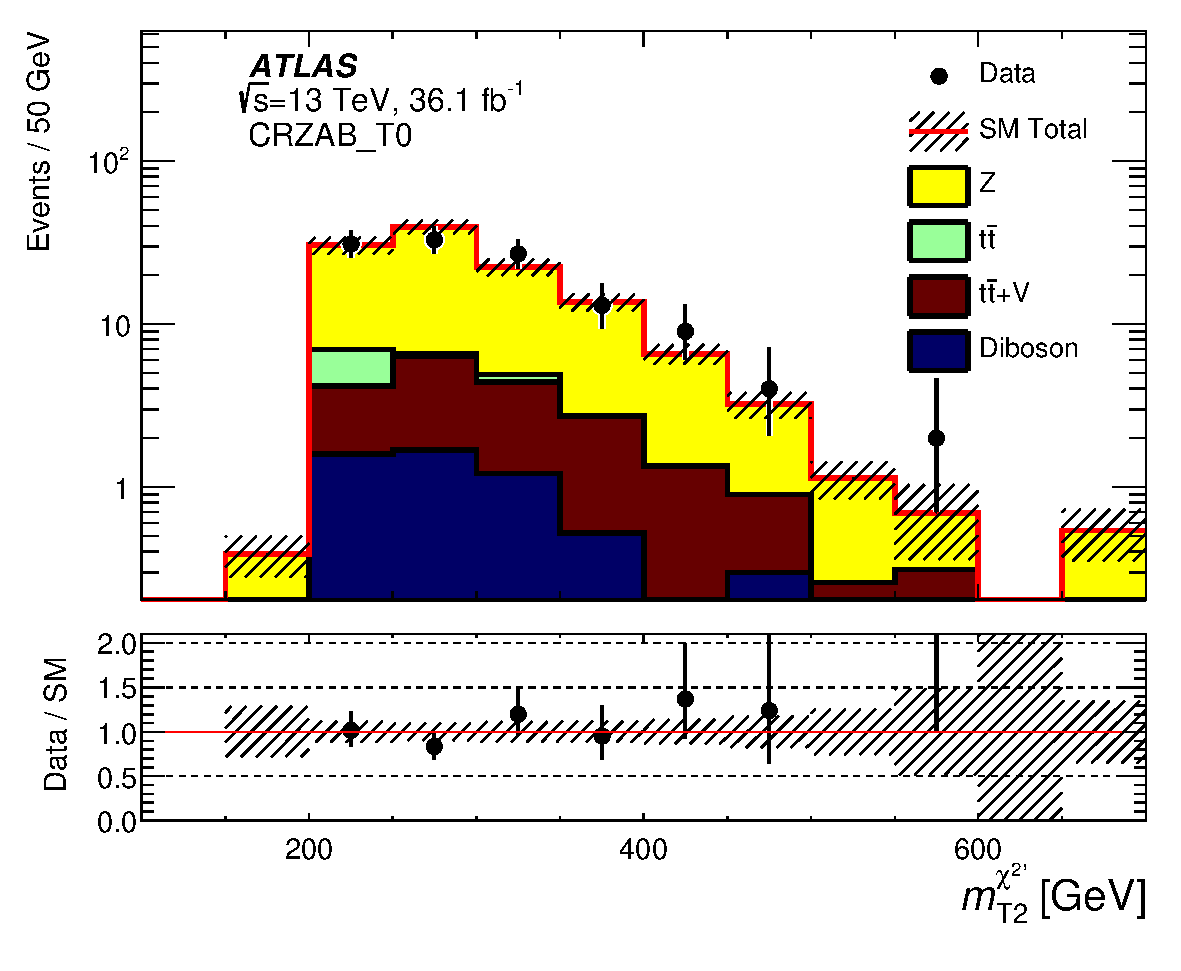
\includegraphics[width=0.48\textwidth]{figures/stop/CRs/Znunu/MT2Chi2Lep_CRZAB_T0_log}}
		    % \subbottom[]{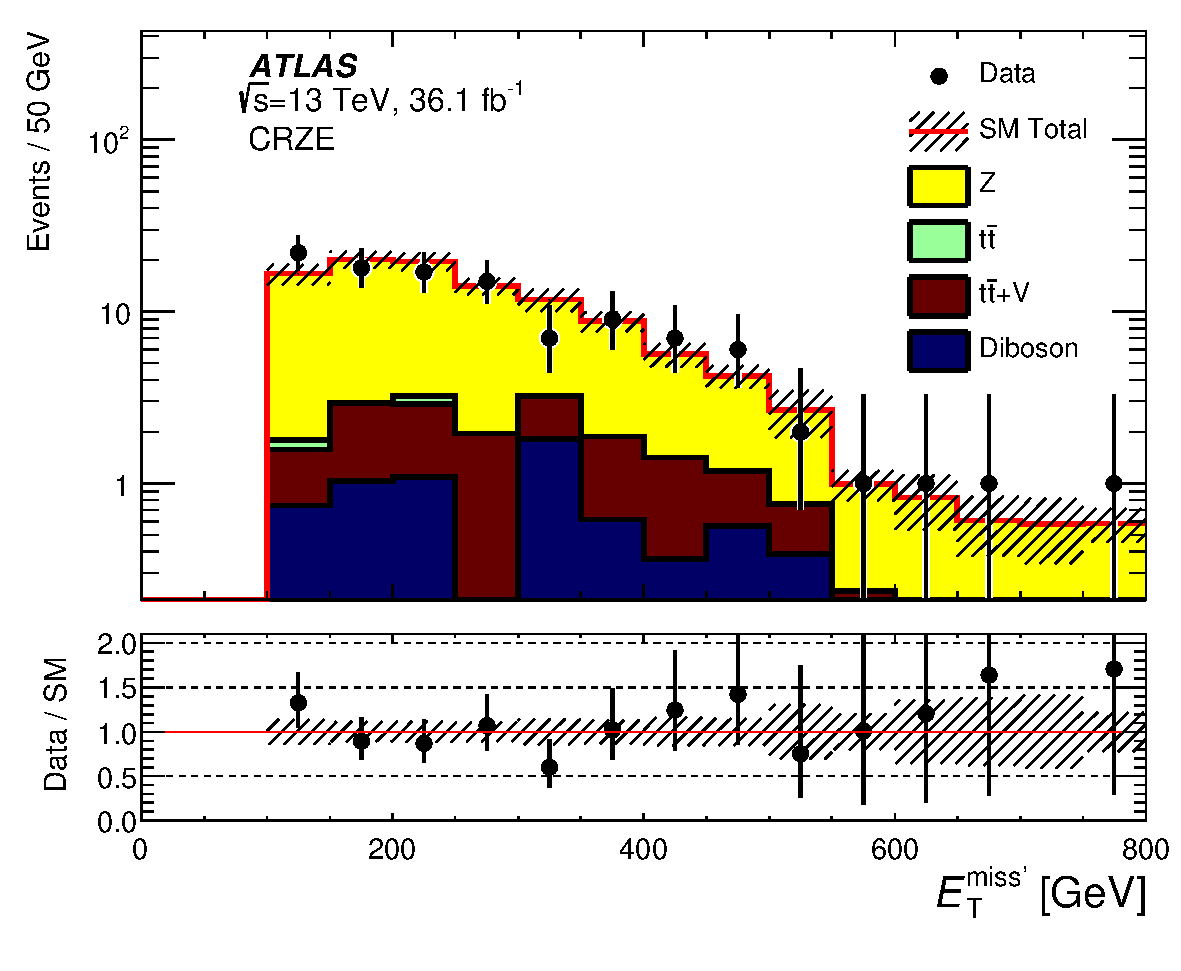
\includegraphics[width=0.48\textwidth]{figures/stop/CRs/Znunu/MetLep_CRZE_log}}
		    \subbottom[]{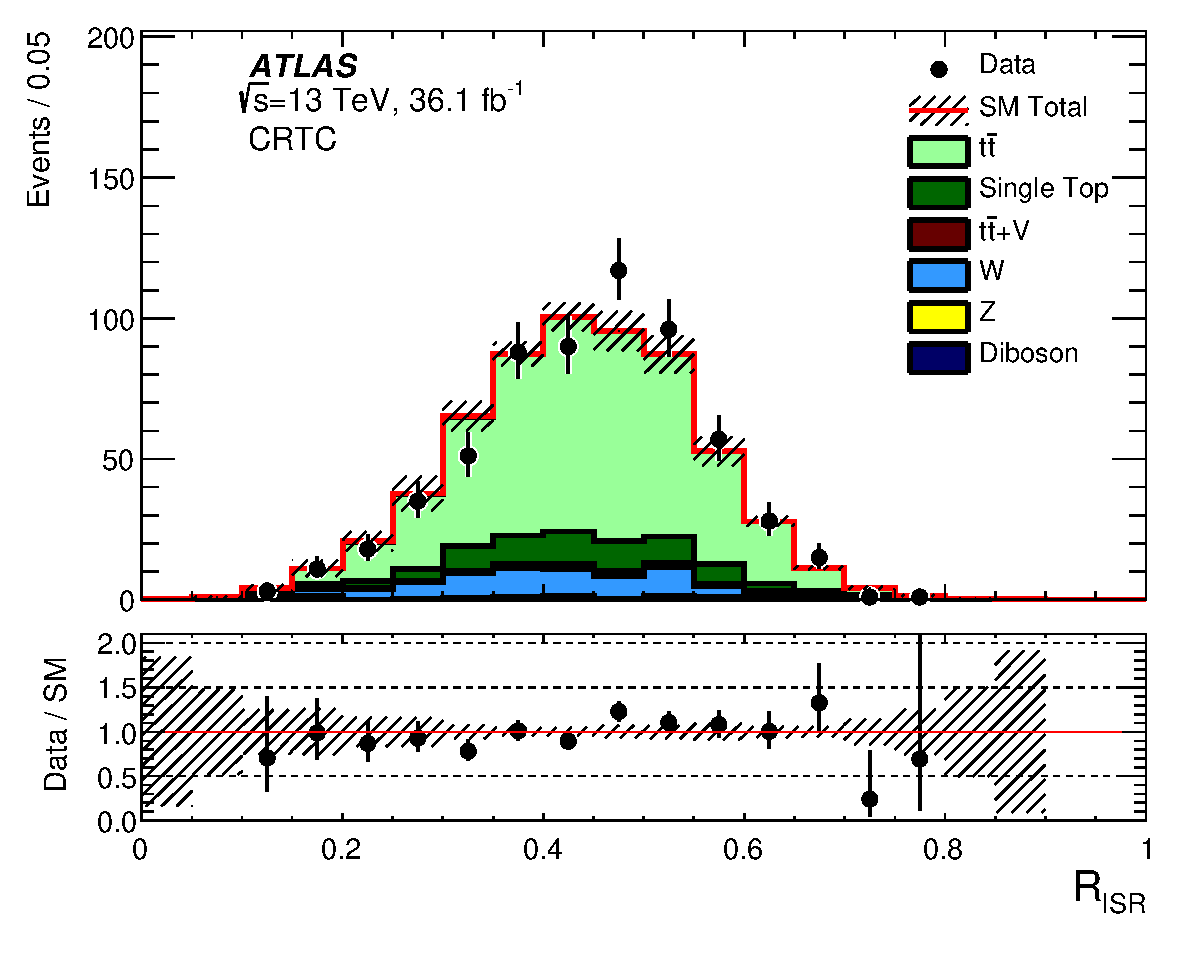
\includegraphics[width=0.48\textwidth]{figures/stop/CRs/ttbar/CA_RISR_CRTopC}}\\
		    \subbottom[]{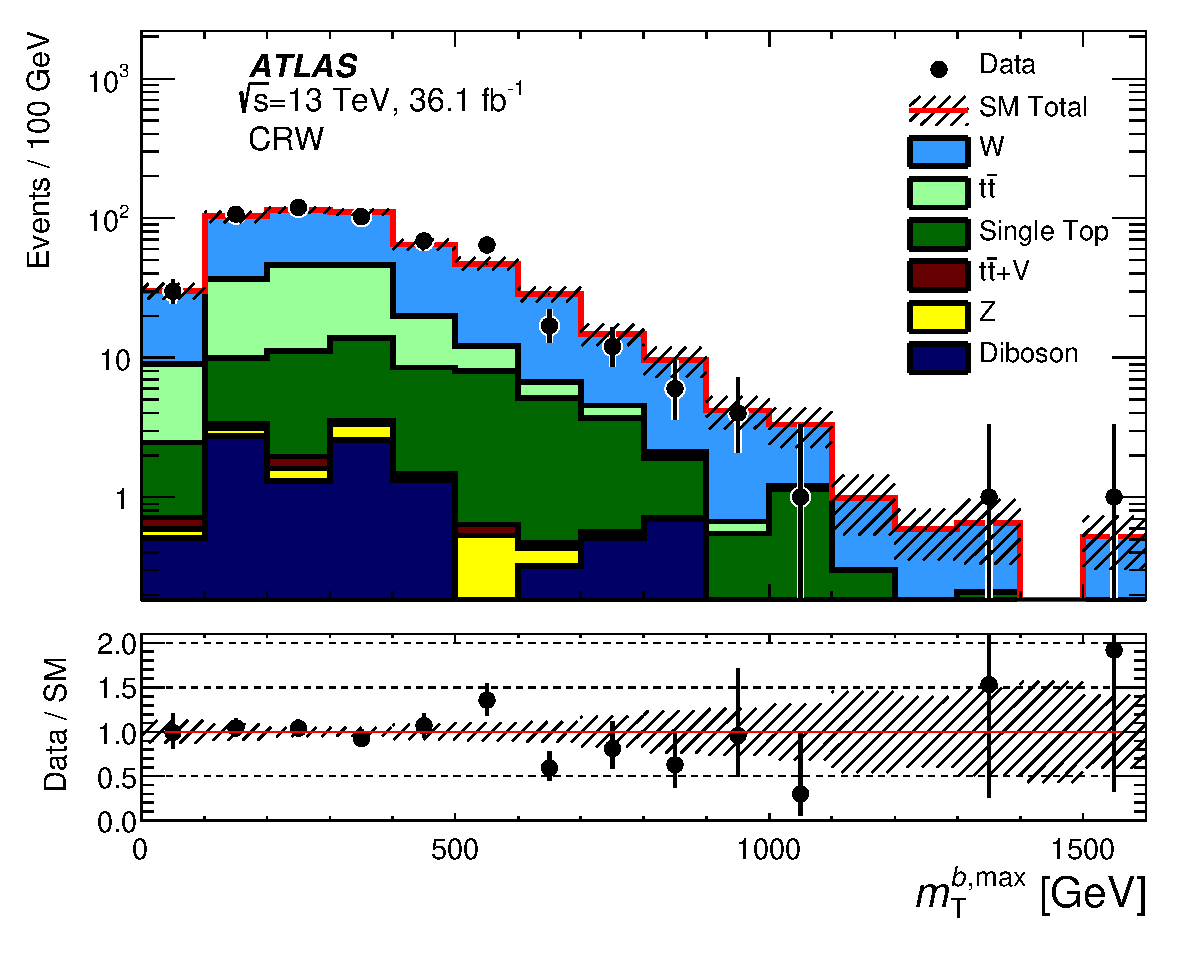
\includegraphics[width=0.48\textwidth]{figures/stop/CRs/Wjets/MtBMax_CRW_log}}
		    \subbottom[]{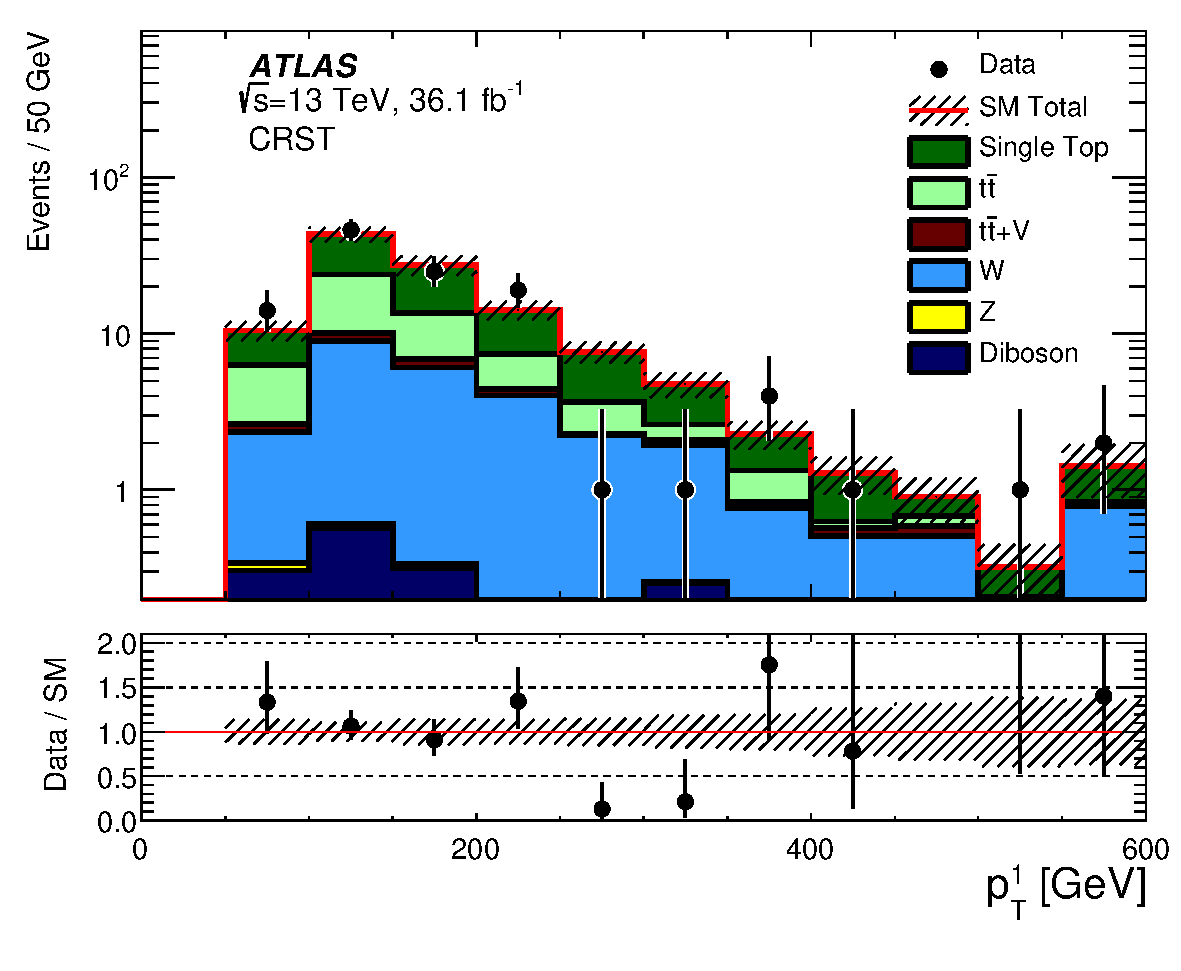
\includegraphics[width=0.48\textwidth]{figures/stop/CRs/singleTop/JetPt_1__CRST_log}}
		    \caption{Distributions of the most relevant variables: (a)~\mttwoprime\ in CRZAB-T0, (b)~\metprime\ in CRZE, (c)~\rISR\ in CRTC, (d)~\mtbmax\ in CRW, (e)~the transverse momentum of the second-leading-\pT\ jet in CRST. The stacked histograms show the \ac{SM} prediction, normalised using scale factors derived from the simultaneous fit to all backgrounds, discussed in Section~\ref{sec:stat_ana}. The ratio of data events to the total \ac{SM} prediction is also shown. The uncertainty band around the \ac{SM} prediction and in the ratio plot illustrates the combination of \ac{MC} statistical and detector-related systematic uncertainties. The rightmost bin includes overflow events~\cite{stop0L}.}
		    \label{fig:CRs}
			\end{figure}

			The result of the simultaneous fit procedure, described in Section~\ref{sec:stat_ana}, performed for each \ac{VR} is shown in Figure~\ref{fig:VRs}, which displays the agreement between data and \ac{MC} predictions. Here, the normalisation factors of the various \ac{SM} background estimation - all between $0.9 - 1.3$ - were used. Additionally, in all the \acp{VR} the signal contamination was checked for all the signals considered that have not yet been excluded. The largest signal contamination is $\sim 25\%$ in the VRTs for top-squark masses below $350$ \GeV\ and in VRZD and VRZE near top-squark masses of $700$ \GeV.

			\begin{figure}[!htb]
			  \begin{center}
			    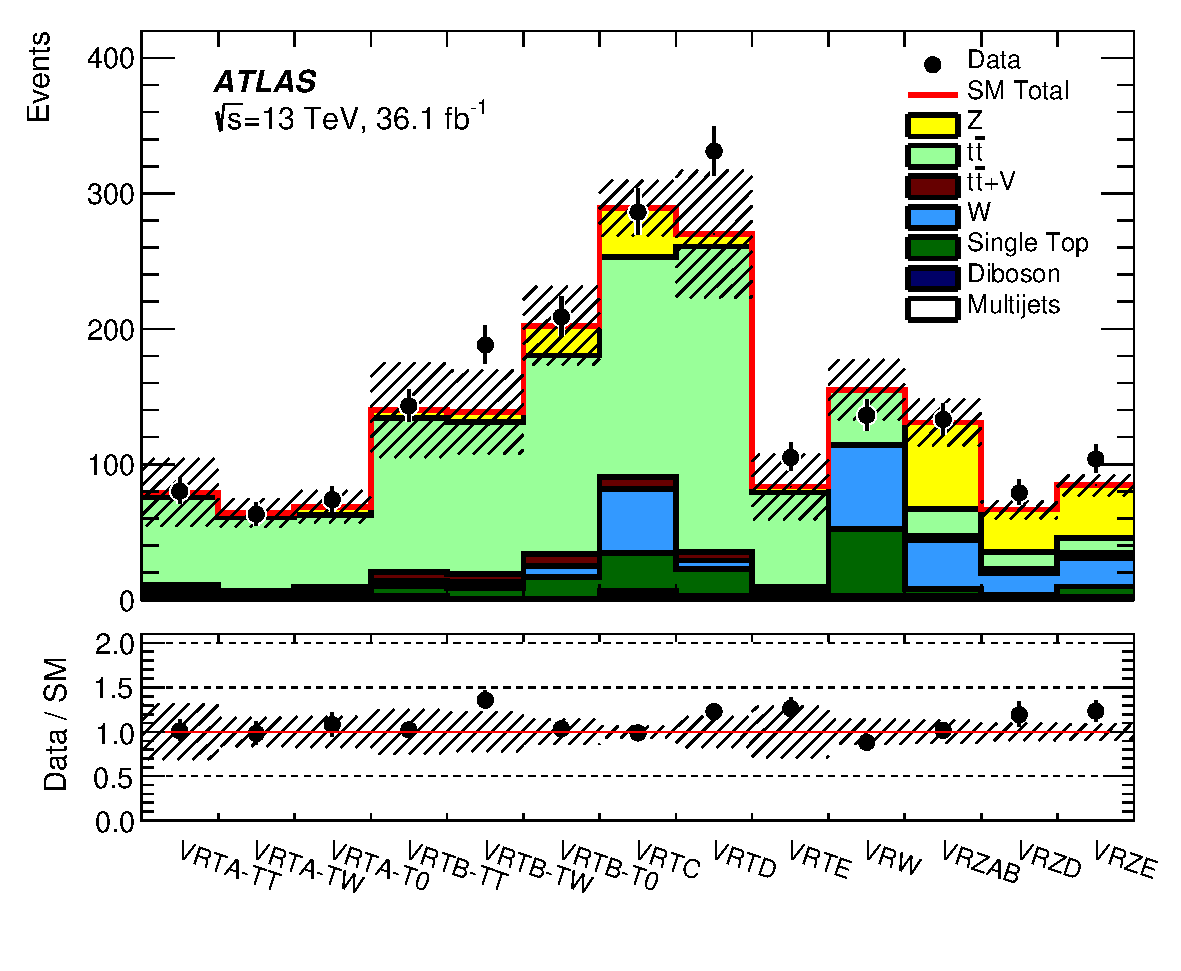
\includegraphics[width=.8\textwidth]{figures/stop/regionSummaryVR}
			    \caption{Yields for all the \acp{VR} after the likelihood fit. The stacked histograms show the \ac{SM} prediction and the uncertainty band around the \ac{SM} prediction shows the total uncertainty, which consists of the \ac{MC} statistical uncertainties, detector-related systematic uncertainties, and theoretical uncertainties in the extrapolation from \ac{CR} to \ac{VR}.} 
			    \label{fig:VRs}
			  \end{center}
			\end{figure}


 		\subsection{Opening Pandora's box: unblinded \acp{SR}}
 		\label{subsec:unblinded_SR}

 			The good agreement found in the \acp{CR} and \acp{VR} gives confidence in the modelling of the relevant \ac{SM} backgrounds and their estimation, therefore the \acp{SR} can now be unblinded. The event data counts are compared to the expected total number of background events in Tables~\ref{tab:srABYields},~\ref{tab:srCYields}, and~\ref{tab:srDEYields}. Figure~\ref{fig:srSummary} shows a summary of all the \ac{SR} yields after having performed the simultaneous likelihood fit.	
			
			\begin{table}[htpb]
				\caption{Observed and expected yields, before and after the fit, for SRA and SRB. The uncertainties include MC statistical uncertainties, detector-related systematic uncertainties, and theoretical uncertainties in the extrapolation from CR to SR~\cite{stop0L}.}
			  \begin{center}
					{\renewcommand{\arraystretch}{1.2}
					\begin{tabular}{lcccccc}
\toprule
 & {\textbf{SRA-TT}} & {\textbf{SRA-TW}} & {\textbf{SRA-T0}} & {\textbf{SRB-TT}} & {\textbf{SRB-TW}} & {\textbf{SRB-T0}}\\ \midrule 
{\textbf{Observed}} & {$11$} & {$9$} & {$18$} & {$38$} & {$53$} & {$206$} \\ \midrule 
{\textbf{Total SM (fit)}} & \multicolumn{1}{c}{$8.6\phantom{0} \pm 2.1\phantom{0}$} & \multicolumn{1}{c}{$9.3\phantom{0} \pm 2.2\phantom{0}$} & \multicolumn{1}{c}{$18.7\phantom{0} \pm 2.7\phantom{0}$} & \multicolumn{1}{c}{$39.3\phantom{0} \pm 7.6\phantom{0}$} & \multicolumn{1}{c}{$52.4\phantom{0} \pm 7.4\phantom{0}$} & \multicolumn{1}{c}{$179\phantom{000} \pm 26\phantom{000}$}\\ \midrule 
{\ttbar} & \multicolumn{1}{c}{$0.71\;_{-\;0.71}^{+\;0.91}$} & \multicolumn{1}{c}{$0.51\;_{-\;0.51}^{+\;0.55}$} & \multicolumn{1}{c}{$\phantom{1}1.31 \pm 0.64$} & \multicolumn{1}{c}{$\phantom{3}7.3\phantom{0} \pm 4.3\phantom{0}$} & \multicolumn{1}{c}{$12.4\phantom{0} \pm 5.9\phantom{0}$} & \multicolumn{1}{c}{$\phantom{1}43\phantom{000} \pm 22\phantom{000}$}\\ 
{\Wjets} & \multicolumn{1}{c}{$0.82 \pm 0.15$} & \multicolumn{1}{c}{$0.89 \pm 0.56$} & \multicolumn{1}{c}{$\phantom{1}2.00 \pm 0.83$} & \multicolumn{1}{c}{$\phantom{3}7.8\phantom{0} \pm 2.8\phantom{0}$} & \multicolumn{1}{c}{$\phantom{5}4.8\phantom{0} \pm 1.2\phantom{0}$} & \multicolumn{1}{c}{$\phantom{1}25.8\phantom{0} \pm \phantom{2}8.8\phantom{0}$}\\ 
{\Zjets} & \multicolumn{1}{c}{$2.5\phantom{0} \pm 1.3\phantom{0}$} & \multicolumn{1}{c}{$4.9\phantom{0} \pm 1.9\phantom{0}$} & \multicolumn{1}{c}{$\phantom{1}9.8\phantom{0} \pm 1.6\phantom{0}$} & \multicolumn{1}{c}{$\phantom{3}9.0\phantom{0} \pm 2.8\phantom{0}$} & \multicolumn{1}{c}{$16.8\phantom{0} \pm 4.1\phantom{0}$} & \multicolumn{1}{c}{$\phantom{1}60.7\phantom{0} \pm \phantom{2}9.6\phantom{0}$}\\ 
{\ttV} & \multicolumn{1}{c}{$3.16 \pm 0.66$} & \multicolumn{1}{c}{$1.84 \pm 0.39$} & \multicolumn{1}{c}{$\phantom{1}2.60 \pm 0.53$} & \multicolumn{1}{c}{$\phantom{3}9.3\phantom{0} \pm 1.7\phantom{0}$} & \multicolumn{1}{c}{$10.8\phantom{0} \pm 1.6\phantom{0}$} & \multicolumn{1}{c}{$\phantom{1}20.5\phantom{0} \pm \phantom{2}3.2\phantom{0}$}\\ 
{Single top} & \multicolumn{1}{c}{$1.20 \pm 0.81$} & \multicolumn{1}{c}{$0.70 \pm 0.42$} & \multicolumn{1}{c}{$\phantom{1}2.9\phantom{0} \pm 1.5\phantom{0}$} & \multicolumn{1}{c}{$\phantom{3}4.2\phantom{0} \pm 2.2\phantom{0}$} & \multicolumn{1}{c}{$\phantom{5}5.9\phantom{0} \pm 2.8\phantom{0}$} & \multicolumn{1}{c}{$\phantom{1}26\phantom{000} \pm 13\phantom{000}$}\\ 
{Dibosons} & \multicolumn{1}{c}{${-} {-}$} & \multicolumn{1}{c}{$0.35 \pm 0.26$} & \multicolumn{1}{c}{${-} {-}$} & \multicolumn{1}{c}{$\phantom{3}0.13 \pm 0.07$} & \multicolumn{1}{c}{$\phantom{5}0.60 \pm 0.43$} & \multicolumn{1}{c}{$\phantom{17}1.04 \pm \phantom{2}0.73$}\\ 
{Multijets} & \multicolumn{1}{c}{$0.21 \pm 0.10$} & \multicolumn{1}{c}{$0.14 \pm 0.09$} & \multicolumn{1}{c}{$\phantom{1}0.12 \pm 0.07$} & \multicolumn{1}{c}{$\phantom{3}1.54 \pm 0.64$} & \multicolumn{1}{c}{$\phantom{5}1.01 \pm 0.88$} & \multicolumn{1}{c}{$\phantom{17}1.8\phantom{0} \pm \phantom{2}1.5\phantom{0}$}\\ \midrule 
{\textbf{Total SM (exp)}} & \multicolumn{1}{c}{$7.1\phantom{3}\phantom{3}$}  & \multicolumn{1}{c}{$7.9\phantom{3}\phantom{3}$}  & \multicolumn{1}{c}{$16.3\phantom{3}\phantom{3}$}  & \multicolumn{1}{c}{$32.4\phantom{3}\phantom{3}$}  & \multicolumn{1}{c}{$46.1\phantom{3}\phantom{3}$}  & \multicolumn{1}{c}{$162\phantom{3}\phantom{2}$} \\  
\bottomrule
\end{tabular}

					}
				\end{center}
				\label{tab:srABYields}
			\end{table}

			\begin{table}[htpb]
			  \caption{Observed and expected yields, before and after the fit.
			The uncertainties include MC statistical uncertainties, detector-related systematic uncertainties, and theoretical uncertainties in the extrapolation from CR to SR~\cite{stop0L}.}
			  \begin{center}
			{\renewcommand{\arraystretch}{1.2}
			\begin{tabular}{lccccc}
\toprule
& {\textbf{SRC1}} & {\textbf{SRC2}} & {\textbf{SRC3}} & {\textbf{SRC4}} & {\textbf{SRC5}}\\ \midrule 
{\textbf{Observed}} & \multicolumn{1}{c}{$20$} & \multicolumn{1}{c}{$22$} & \multicolumn{1}{c}{$22$} & \multicolumn{1}{c}{$1$} & \multicolumn{1}{c}{$0$} \\ \midrule
{\textbf{Total SM (fit)}} & {$20.6\phantom{0} \pm 6.5\phantom{0}$} & {$27.6\phantom{0} \pm 4.9\phantom{0}$} & {$18.9\phantom{0} \pm 3.4\phantom{0}$} & {$7.7\phantom{0} \pm 1.2\phantom{0}$} & {$0.91 \pm 0.73$}\\ \midrule 
{\ttbar} & 	{$12.9\phantom{0} \pm 5.9\phantom{0}$} & \multicolumn{1}{c}{$22.1\phantom{0} \pm 4.3\phantom{0}$} & \multicolumn{1}{c}{$14.6\phantom{0} \pm 3.2\phantom{0}$} & \multicolumn{1}{c}{$4.91 \pm 0.97$} & \multicolumn{1}{c}{$0.63\;_{-\;0.63}^{+\;0.70}$}\\ 
{\Wjets} & \multicolumn{1}{c}{$\phantom{2}0.80 \pm 0.37$} & \multicolumn{1}{c}{$\phantom{2}1.93 \pm 0.49$} & \multicolumn{1}{c}{$\phantom{1}1.91 \pm 0.62$} & \multicolumn{1}{c}{$1.93 \pm 0.46$} & \multicolumn{1}{c}{$0.21 \pm 0.12$}\\ 
{\Zjets} & \multicolumn{1}{c}{${-} {-}$} & \multicolumn{1}{c}{${-} {-}$} & \multicolumn{1}{c}{${-} {-}$} & \multicolumn{1}{c}{${-} {-}$} & \multicolumn{1}{c}{${-} {-}$}\\ 
{\ttV} & \multicolumn{1}{c}{$\phantom{2}0.29 \pm 0.16$} & \multicolumn{1}{c}{$\phantom{2}0.59 \pm 0.38$} & \multicolumn{1}{c}{$\phantom{1}0.56 \pm 0.31$} & \multicolumn{1}{c}{$0.08 \pm 0.08$} & \multicolumn{1}{c}{$0.06 \pm 0.02$}\\ 
{Single top} & \multicolumn{1}{c}{$\phantom{2}1.7\phantom{0} \pm 1.3\phantom{0}$} & \multicolumn{1}{c}{$\phantom{2}1.2\phantom{0}\;_{-\;1.2}^{+\;1.4\phantom{0}}$} & \multicolumn{1}{c}{$\phantom{1}1.22 \pm 0.69$} & \multicolumn{1}{c}{$0.72 \pm 0.37$} & \multicolumn{1}{c}{${-} {-}$}\\ 
{Dibosons} & \multicolumn{1}{c}{$\phantom{2}0.39 \pm 0.33$} & \multicolumn{1}{c}{$\phantom{2}0.21\;_{-\;0.21}^{+\;0.23}$} & \multicolumn{1}{c}{$\phantom{1}0.28 \pm 0.18$} & \multicolumn{1}{c}{${-} {-}$} & \multicolumn{1}{c}{${-} {-}$}\\ 
{Multijets} & \multicolumn{1}{c}{$\phantom{2}4.6\phantom{0} \pm 2.4\phantom{0}$} & \multicolumn{1}{c}{$\phantom{2}1.58 \pm 0.77$} & \multicolumn{1}{c}{$\phantom{1}0.32 \pm 0.17$} & \multicolumn{1}{c}{$0.04 \pm 0.02$} & \multicolumn{1}{c}{${-} {-}$}\\ \midrule
{\textbf{Total SM (exp)}} & \multicolumn{1}{c}{$25.4\phantom{3}\phantom{3}$}  & \multicolumn{1}{c}{$36.0\phantom{3}\phantom{3}$}  & \multicolumn{1}{c}{$24.2\phantom{3}\phantom{3}$}  & \multicolumn{1}{c}{$9.2\phantom{3}\phantom{3}$}  & \multicolumn{1}{c}{$1.1\phantom{3}\phantom{4}$} \\ 
\bottomrule
\end{tabular}

			}
			\end{center}
			\label{tab:srCYields}
			\end{table}

			\begin{table}[htpb]
			  \caption{Observed and expected yields, before and after the fit, for SRD and SRE.
			The uncertainties include MC statistical uncertainties, detector-related systematic uncertainties, and theoretical uncertainties in the extrapolation from CR to SR~\cite{stop0L}.}
			  \begin{center}
			{\renewcommand{\arraystretch}{1.2}
			\begin{tabular}{lccc}
\toprule
 & {\textbf{SRD-low}} & {\textbf{SRD-high}} & {\textbf{SRE}}\\ \midrule 
{\textbf{Observed}} & \multicolumn{1}{c}{$27$} & \multicolumn{1}{c}{$11$} & \multicolumn{1}{c}{$3$} \\ \midrule
{\textbf{Total SM (fit)}} & \multicolumn{1}{c}{$25.1\phantom{0} \pm 6.2\phantom{0}$} & \multicolumn{1}{c}{$8.5\phantom{0} \pm 1.5\phantom{0}$} & \multicolumn{1}{c}{$3.64 \pm 0.79$}\\ \midrule 
{\ttbar} & \multicolumn{1}{c}{$\phantom{2}3.3\phantom{0} \pm 3.3\phantom{0}$} & \multicolumn{1}{c}{$0.98 \pm 0.88$} & \multicolumn{1}{c}{$0.21\;_{-\;0.21}^{+\;0.39}$}\\ 
{\Wjets} & \multicolumn{1}{c}{$\phantom{2}6.1\phantom{0} \pm 2.9\phantom{0}$} & \multicolumn{1}{c}{$1.06 \pm 0.34$} & \multicolumn{1}{c}{$0.52 \pm 0.27$}\\ 
{\Zjets} & \multicolumn{1}{c}{$\phantom{2}6.9\phantom{0} \pm 1.5\phantom{0}$} & \multicolumn{1}{c}{$3.21 \pm 0.62$} & \multicolumn{1}{c}{$1.36 \pm 0.25$}\\ 
{\ttV} & \multicolumn{1}{c}{$\phantom{2}3.94 \pm 0.85$} & \multicolumn{1}{c}{$1.37 \pm 0.32$} & \multicolumn{1}{c}{$0.89 \pm 0.19$}\\ 
{Single top} & \multicolumn{1}{c}{$\phantom{2}3.8\phantom{0} \pm 2.1\phantom{0}$} & \multicolumn{1}{c}{$1.51 \pm 0.74$} & \multicolumn{1}{c}{$0.66 \pm 0.49$}\\ 
{Dibosons} & \multicolumn{1}{c}{${-} {-}$} & \multicolumn{1}{c}{${-} {-}$} & \multicolumn{1}{c}{${-} {-}$}\\ 
{Multijets} & \multicolumn{1}{c}{$\phantom{2}1.12 \pm 0.37$} & \multicolumn{1}{c}{$0.40 \pm 0.15$} & \multicolumn{1}{c}{${-} {-}$}\\ \midrule 
{\textbf{Total SM (exp.)}} & \multicolumn{1}{c}{$22.4\phantom{3}\phantom{3}$}  & \multicolumn{1}{c}{$7.7\phantom{3}\phantom{3}$}  & \multicolumn{1}{c}{$3.02\phantom{3}\phantom{4}$} \\ 
\midrule
\end{tabular}

			}
			\end{center}
			\label{tab:srDEYields}
			\end{table}

			The analysis yielded no significant excess above the \ac{SM} prediction in any of the \acp{SR}, as it can be seen in Figure~\ref{fig:srSummary}. The smallest $p$-values are $27\%$, $27\%$, and $29\%$ for SRB-T0, SRD-high, and SRA-TT, respectively. The largest deficit in the data is observed in SRC4 where only one event is observed against $7.7$ expected background events and this is probably due to the very low statistics.

			\begin{figure}[htpb]
			  \begin{center}
			    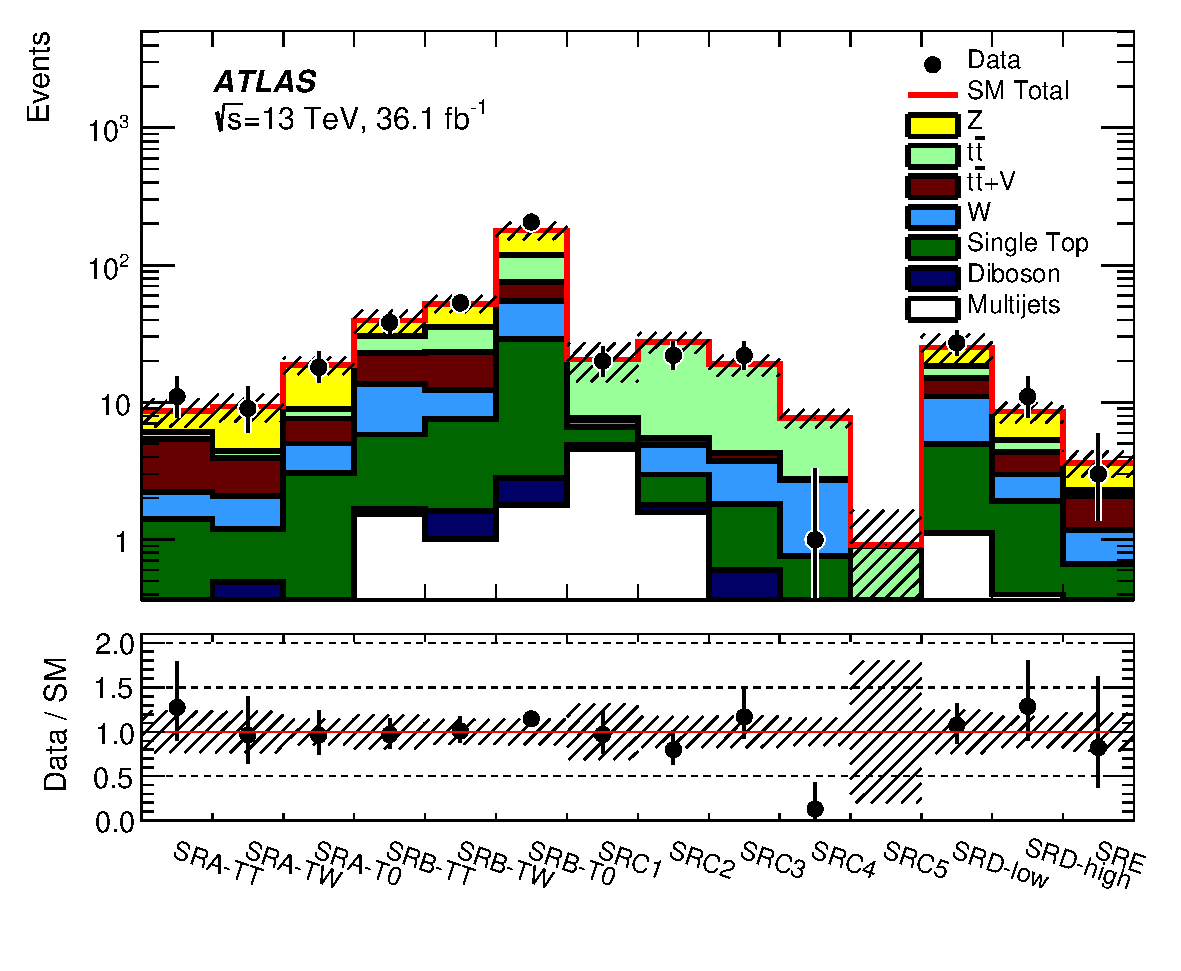
\includegraphics[width=0.8\textwidth]{stop/fit/regionSummaryLog}
			    \caption{Yields for all signal regions after the likelihood fit. The stacked histograms show the SM prediction and the hatched uncertainty band around the SM prediction shows total uncertainty, which consists of the MC statistical uncertainties, detector-related systematic uncertainties, and theoretical uncertainties in the extrapolation from CR to SR~\cite{stop0L}.} 
			    \label{fig:srSummary}
			  \end{center}
			\end{figure}

			Figure~\ref{fig:SRs} shows the $N-1$ distributions, obtained by applying all the \ac{SR} selections but the cut on the variable plotted, of \met, \mttwo, \mtbmax, \mt, \rISR, and \HT, for the various \acp{SR}, with \rISR\ being shown combining SRC1--5. The background predictions in these distributions are scaled to the values determined from the simultaneous fit. A good data-SM prediction agreement is observed across the whole kinematical range in the displayed plots, confirming once again the reliability of the presented background estimation strategy. 

			\begin{figure}[htpb]
			  \begin{center}
			    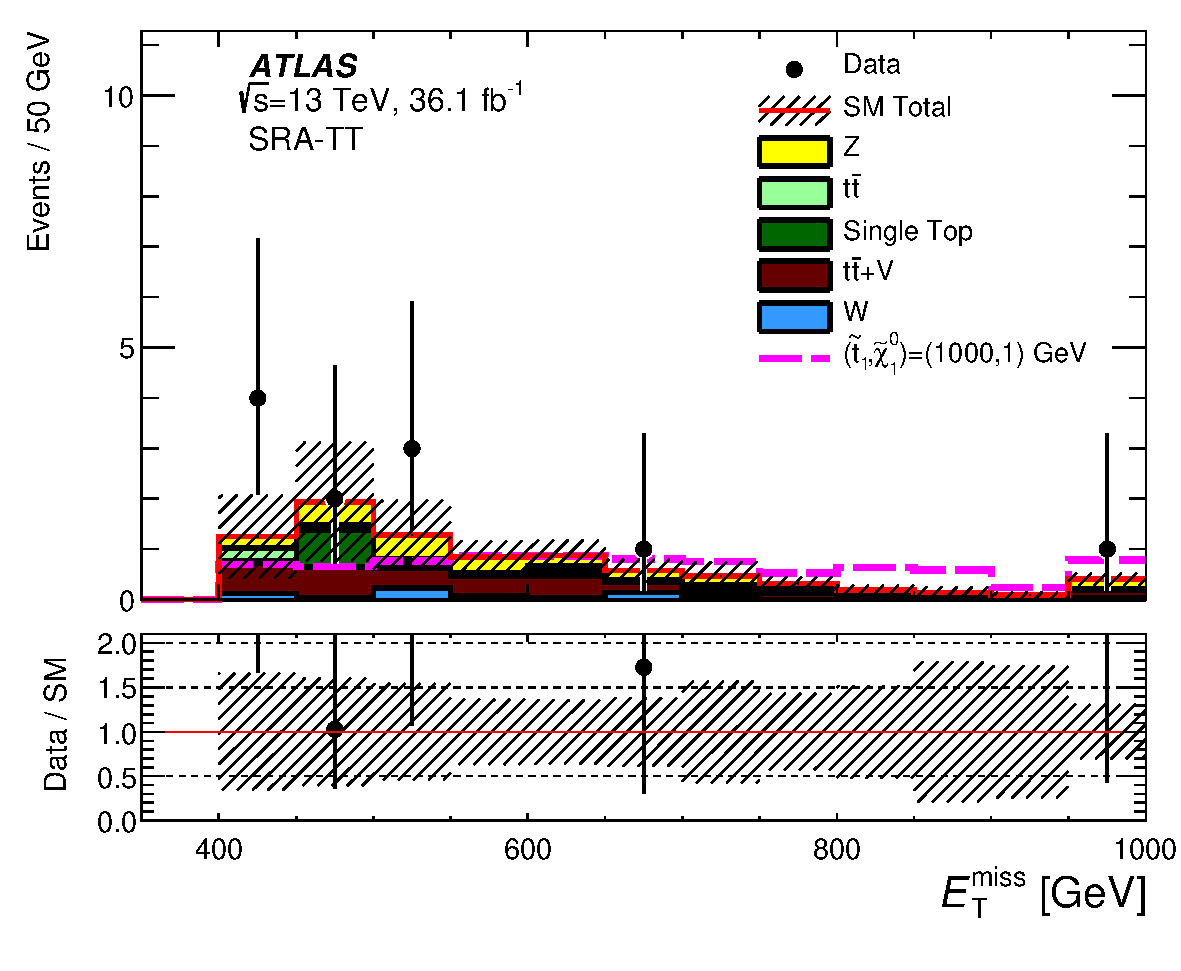
\includegraphics[width=0.49\textwidth]{stop/SRA/Met_SRA_TT}
			    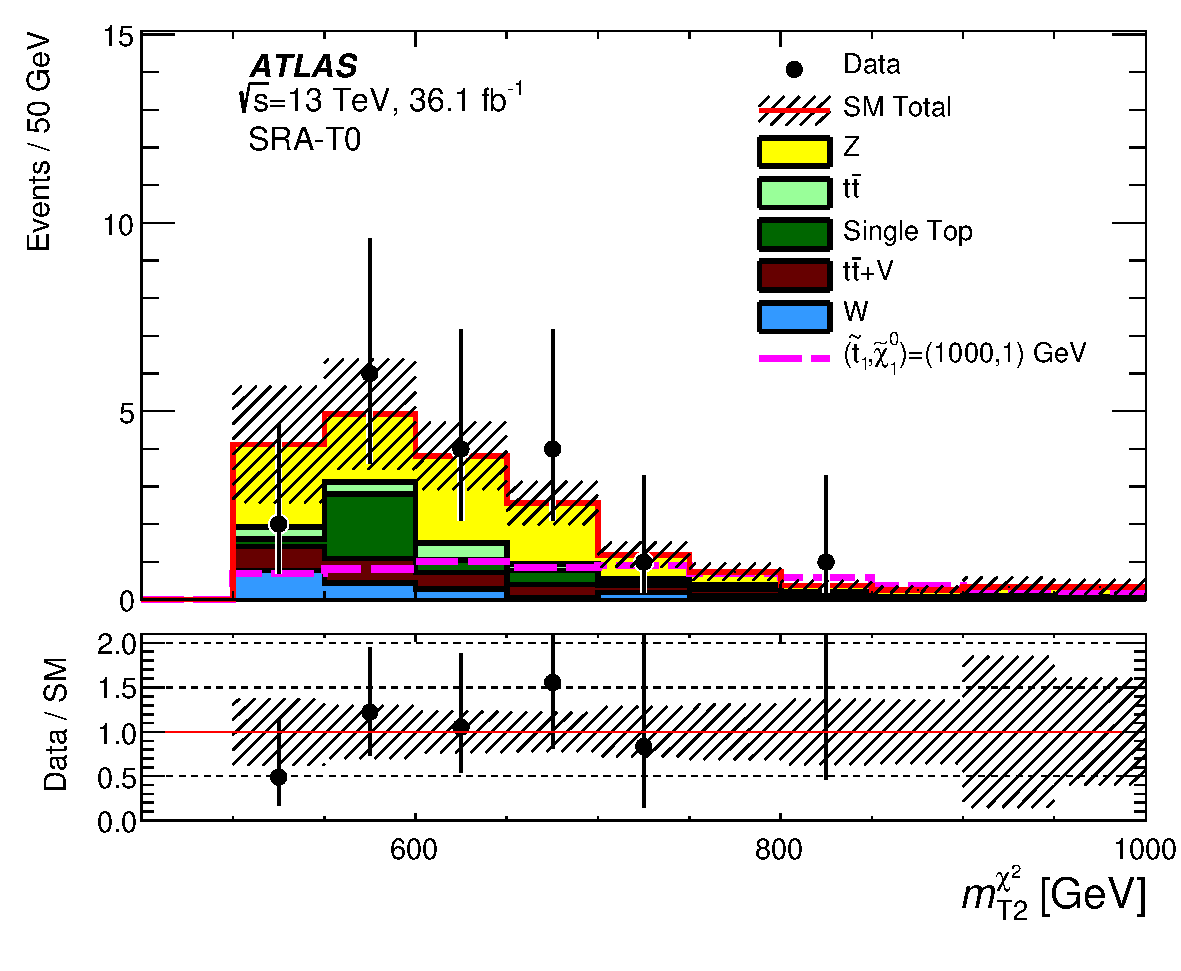
\includegraphics[width=0.49\textwidth]{stop/SRA/MT2Chi2_SRA_T0}\\%\hspace{0.05\textwidth}
			    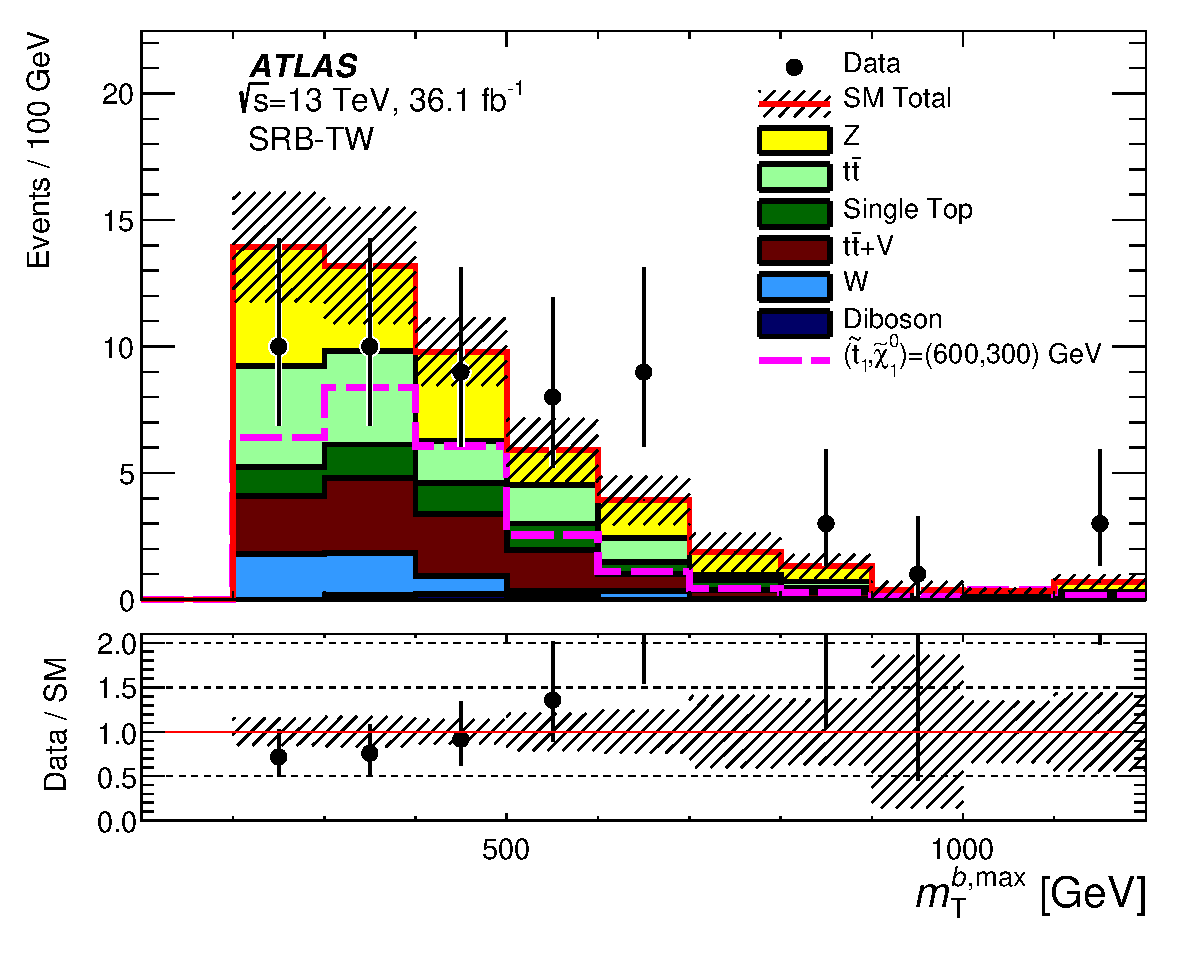
\includegraphics[width=0.49\textwidth]{stop/SRB/MtBMax_SRB_TW}
			    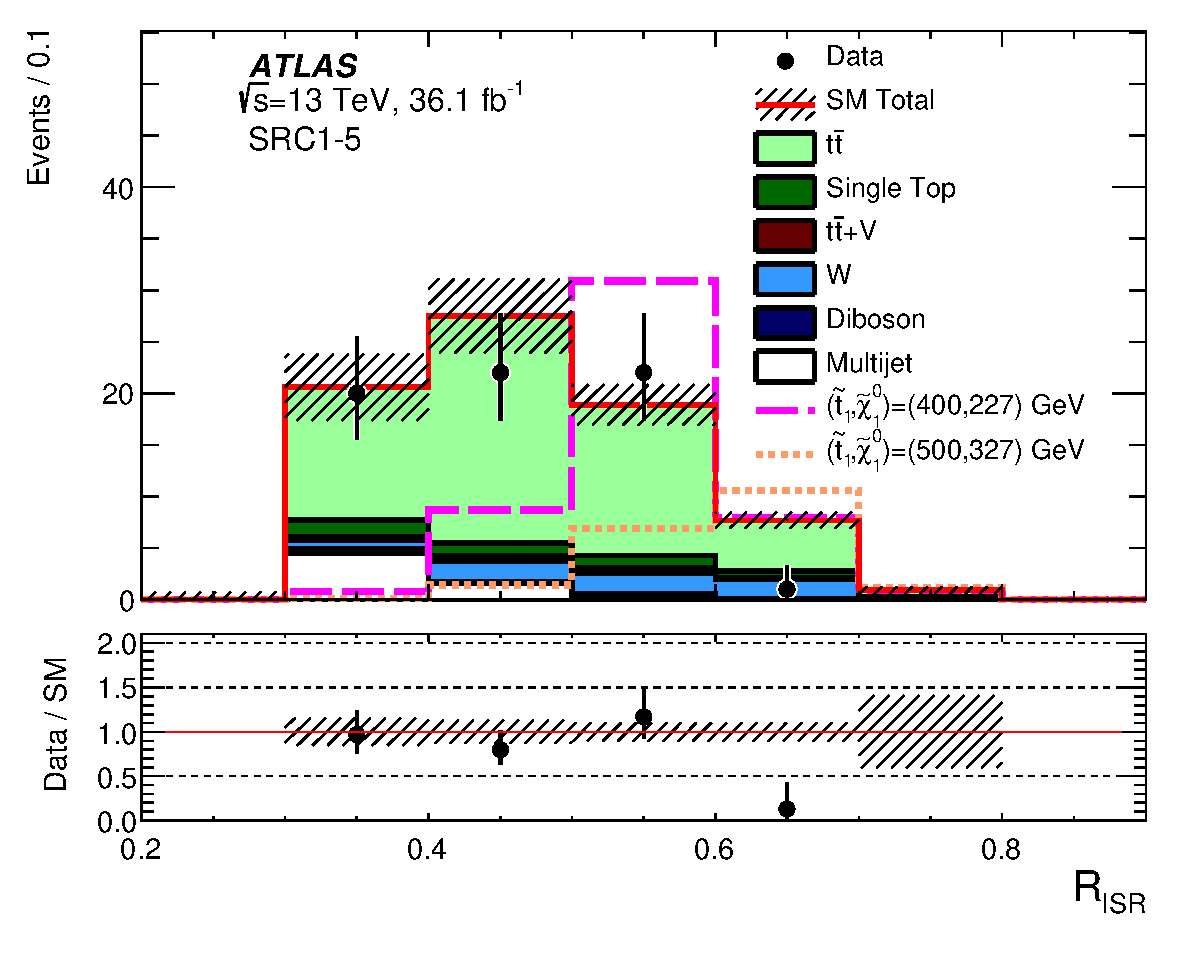
\includegraphics[width=0.49\textwidth]{stop/SRC/CA_RISR_SRC1_5}\\%\hspace{0.05\textwidth}
			    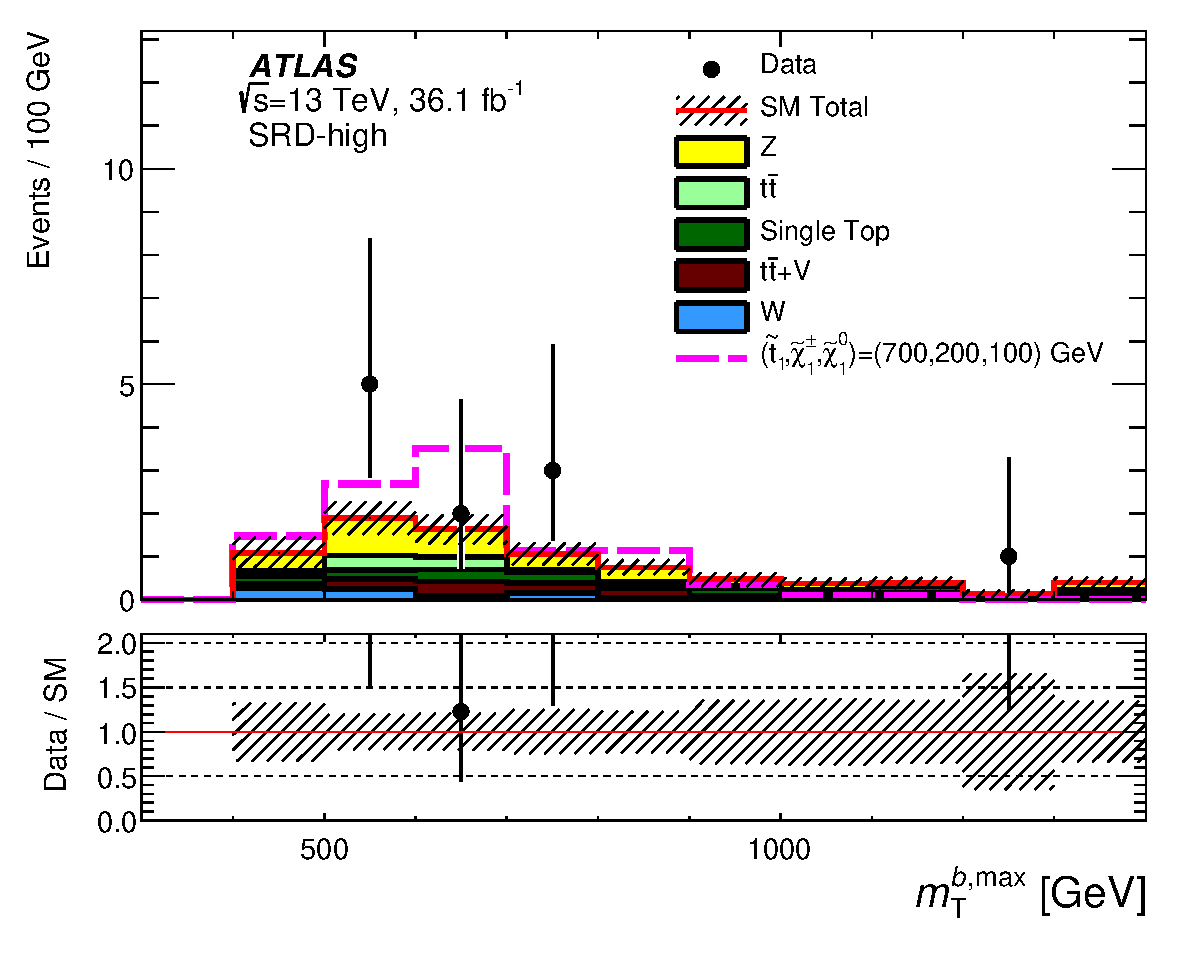
\includegraphics[width=0.49\textwidth]{stop/SRD/MtBMax_SRD_high}
			    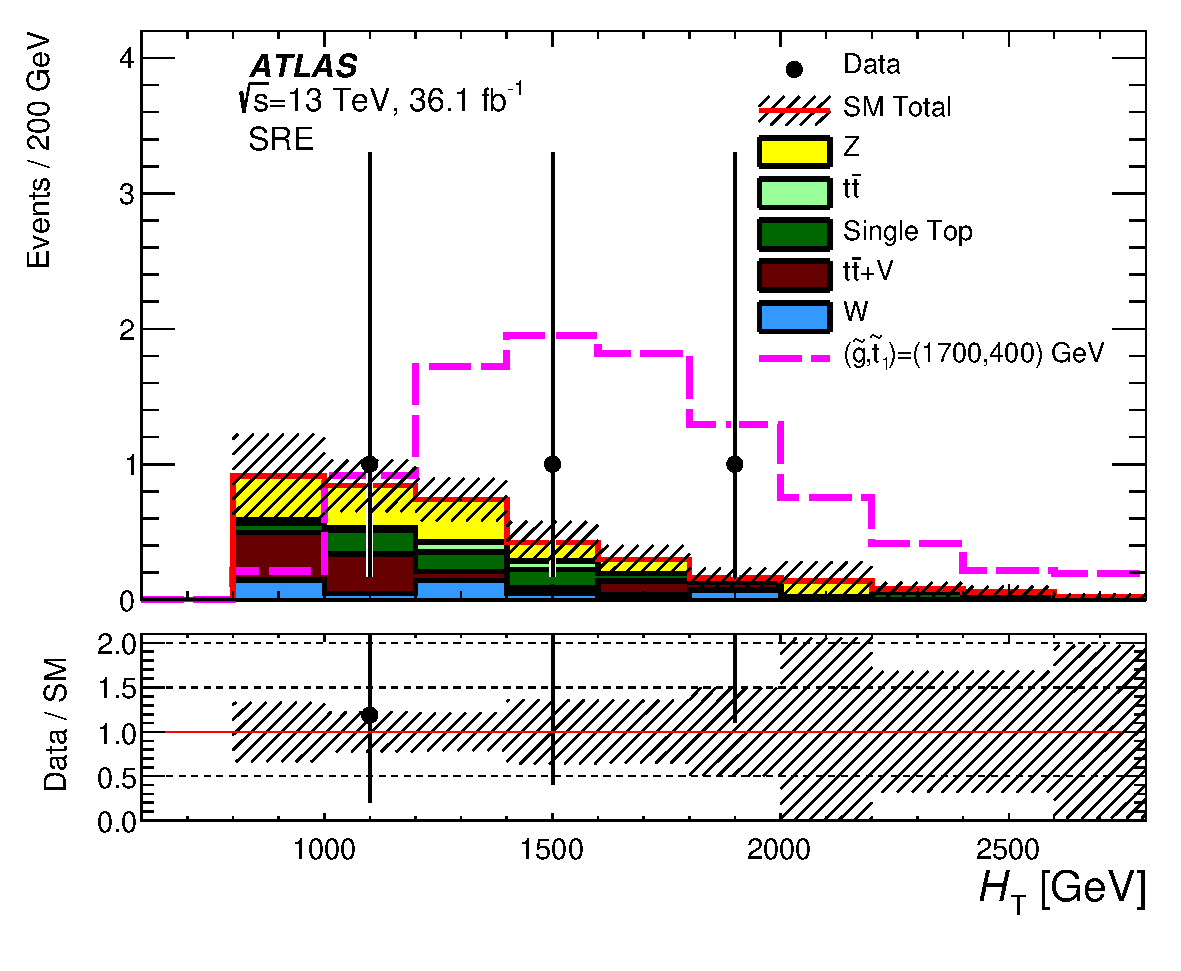
\includegraphics[width=0.49\textwidth]{stop/SRE/Ht_SRE}
			    \caption{Distributions of \met\ for SRA-TT, \mttwo\ for SRA-T0, \mtbmax\ for SRB-TW, \rISR\ for SRC1--5, \mtbmax\ for SRD-high and \HT\ for SRE obtained after having performed the likelihood fit. The stacked histograms show the SM prediction and the hatched uncertainty band around the SM prediction shows the MC statistical and detector-related systematic uncertainties. For each variable, the distribution for a representative signal point is shown~\cite{stop0L}.}
			    \label{fig:SRs}
			  \end{center}
			\end{figure}



 		\subsection{Setting the limits}
 		\label{subsec:limitset}

			As no excess over the \ac{SM} is observed in any of the investigated \acp{SR}, exclusion limits are set. In particular, the $\mathrm{CL}_s$ method, discussed in Section~\ref{sec:stat_ana}, is used to perform the exclusion fits. Model-independent limits on the visible \ac{BSM} cross section, defined as $\sigma_{\mathrm{vis}} = S^{95}_{\textnormal{obs}}/\int\!\!{\mathcal L}\,dt$, where $S^{95}_{\textnormal{obs}}$ is the 95\% CL upper limit on the number of signal events, are reported in Table~\ref{tab:upLimits}.

			\begin{table}[htpb]
				\caption{Left to right: 95\% CL upper limits on the average visible cross section ($\langle\sigma A \epsilon\rangle_{\mathrm obs}^{95}$) where the average comes from possibly multiple production channels and on the number of signal events ($S_{\mathrm obs}^{95}$ ).  The third column ($S_{\mathrm exp}^{95}$) shows the 95\% CL upper limit on the number of signal events, given the expected number (and $\pm 1\sigma$ excursions of the expected number) of background events. The discovery $p$-value ($p$) and the corresponding significance ($Z$) are shown in the last column~\cite{stop0L}.}
				\label{tab:upLimits}
				\begin{center}
		    	{\renewcommand{\arraystretch}{1.3}
\begin{tabular*}{\textwidth}{@{\extracolsep{\fill}}lccccc}
\noalign{\smallskip}\toprule\noalign{\smallskip}
{\textbf{Signal channel}}                        & $\langle{\mathrm{\sigma}} A \epsilon\rangle_{\mathrm{obs}}^{95}$ [fb]  &  $S_{\mathrm{obs}}^{95}$  & $S_{\mathrm{exp}}^{95}$ & $p$ ($Z$)  \\
\noalign{\smallskip}\midrule\noalign{\smallskip}

SRA-TT    & $0.30$ &  $11.0$ & $ { 8.7 }^{ +3.0 }_{ -1.4 }$ & $ 0.23$~$(0.74)$ \\%
SRA-TW    & $0.27$ &  $9.6$ & $ { 9.6 }^{ +2.8 }_{ -2.1 }$ & $ 0.50$~$(0.00)$ \\%
SRA-T0    & $0.31$ &  $11.2$ & $ { 11.5 }^{ +3.8 }_{ -2.0 }$ & $ 0.50$~$(0.00)$ \\%
SRB-TT    & $0.54$ &  $19.6$ & $ { 20.0 }^{ +6.5 }_{ -4.9 }$ & $ 0.50$~$(0.00)$ \\%
SRB-TW    & $0.60$ &  $21.7$ & $ { 21.0 }^{ +7.3 }_{ -4.3 }$ & $ 0.50$~$(0.00)$ \\%
SRB-T0    & $2.19$ &  $80$ & $ { 58 }^{ +23 }_{ -17 }$ & $ 0.13$~$(1.15)$ \\%
SRC1    & $0.42$ &  $15.1$ & $ { 15.8 }^{ +4.8 }_{ -3.5 }$ & $ 0.50$~$(0.00)$ \\%
SRC2    & $0.31$ &  $11.2$ & $ { 13.9 }^{ +5.9 }_{ -3.6 }$ & $ 0.50$~$(0.00)$ \\%
SRC3    & $0.42$ &  $15.3$ & $ { 12.3 }^{ +4.7 }_{ -3.4 }$ & $ 0.27$~$(0.62)$ \\%
SRC4    & $0.10$ &  $3.5$ & $ { 6.7 }^{ +2.8 }_{ -1.8 }$ & $ 0.50$~$(0.00)$ \\%
SRC5    & $0.09$ &  $3.2$ & $ { 3.0 }^{ +1.1 }_{ -0.1 }$ & $ 0.23$~$(0.74)$ \\%
SRD-low    & $0.50$ &  $17.9$ & $ { 16.4 }^{ +6.3 }_{ -4.0 }$ & $ 0.36$~$(0.35)$ \\%
SRD-high    & $0.30$ &  $10.9$ & $ { 8.0 }^{ +3.4 }_{ -1.3 }$ & $ 0.21$~$(0.79)$ \\%
SRE    & $0.17$ &  $6.1$ & $ { 6.4 }^{ +1.4 }_{ -2.4 }$ & $ 0.50$~$(0.00)$ \\%

\noalign{\smallskip}\bottomrule\noalign{\smallskip}
\end{tabular*}
}
%\end{table}
%

				\end{center}
			\end{table}

			The detector acceptance multiplied by the efficiency, $A\cdot\epsilon$, is calculated for all the \acp{SR} and the equivalent benchmark points. In particular, for signal regions designed to aim at the high-energy final states (SRA and SRE) $A\cdot\epsilon$ is estimated to be $9\%$ and $6\%$ for their respective signal benchmark points: $\mstop=1000\gev,\mLSP=1\gev$; and $m_{\gluino} = 1700\GeV, \mstop=400\GeV, \mLSP=395\GeV$. In SRB, SRD-low, and SRD-high the estimates of $A\cdot \epsilon$ is $1.4\%$, $0.05\%$, and 0$.5\%$ for $\mstop=600\gev,\mLSP=300\gev$; $\mstop =400\GeV, m_{\chinoonepm}=100\GeV, \mLSP=50\GeV$; and $\mstop =700\GeV, m_{\chinoonepm}=200\GeV, \mLSP=100\GeV$, where the branching ratio, $B$($\stop\to b \chinoonepm$) = $100\%$ is assumed for the SRD samples. The combination of SRC1--5 through the \rISR\ windows shows an $A\cdot\epsilon$ of $0.08\%$ for $\mstop= 400\GeV, \mLSP=227\GeV$. Furthermore, orthogonal signal subregions, namely SRA-TT, SRA-TW, and SRA-T0, are statistically combined by multiplying their likelihood functions, and the same procedure is applied to the SRB and SRC signal subregions. For the overlapping \acp{SR} SRD-low and SRD-high, the signal region with the smallest expected CL$_\mathrm{s}$ value is chosen for each signal model. Once the signal subregions are combined or chosen, the signal region with the smallest expected CL$_\mathrm{s}$ is chosen for each signal model in the $\stop$--$\ninoone$ signal grid. The expected limits are determined by setting the nominal event yield in each \ac{SR} to the mean background expectation; contours that correspond to $\pm1\sigma$ uncertainties in the background estimates, $\sigma_{\mathrm{exp}}$, are also evaluated. The observed event yields determine the observed limits for each SR; these are evaluated for the nominal signal cross sections as well as for $\pm1\sigma$ theory uncertainties in those cross sections, denoted by $\sigma^{\mathrm{SUSY}}_{\mathrm{theory}}$. 

			The observed (solid red line) and expected (solid blue line) exclusion contours at $95\%$ CL in the \stop--\ninoone\ mass plane are shown in Figure~\ref{fig:SRABC_exclusion}. The data excluded top-squark masses between \stopLimLowLSPLow\ and \stopLimLowLSPHigh\ \GeV\ for $\ninoone$ masses below $160\GeV$, extending Run-1 limits by $260$~\GeV. The newly explored ``diagonal'' case, where $\mstop\approx m_t+\mLSP$, was also added. Here top-squark masses in the range \stopLimDiag\ \GeV\ are excluded. 

			\begin{figure}[htpb]
			  \begin{center} 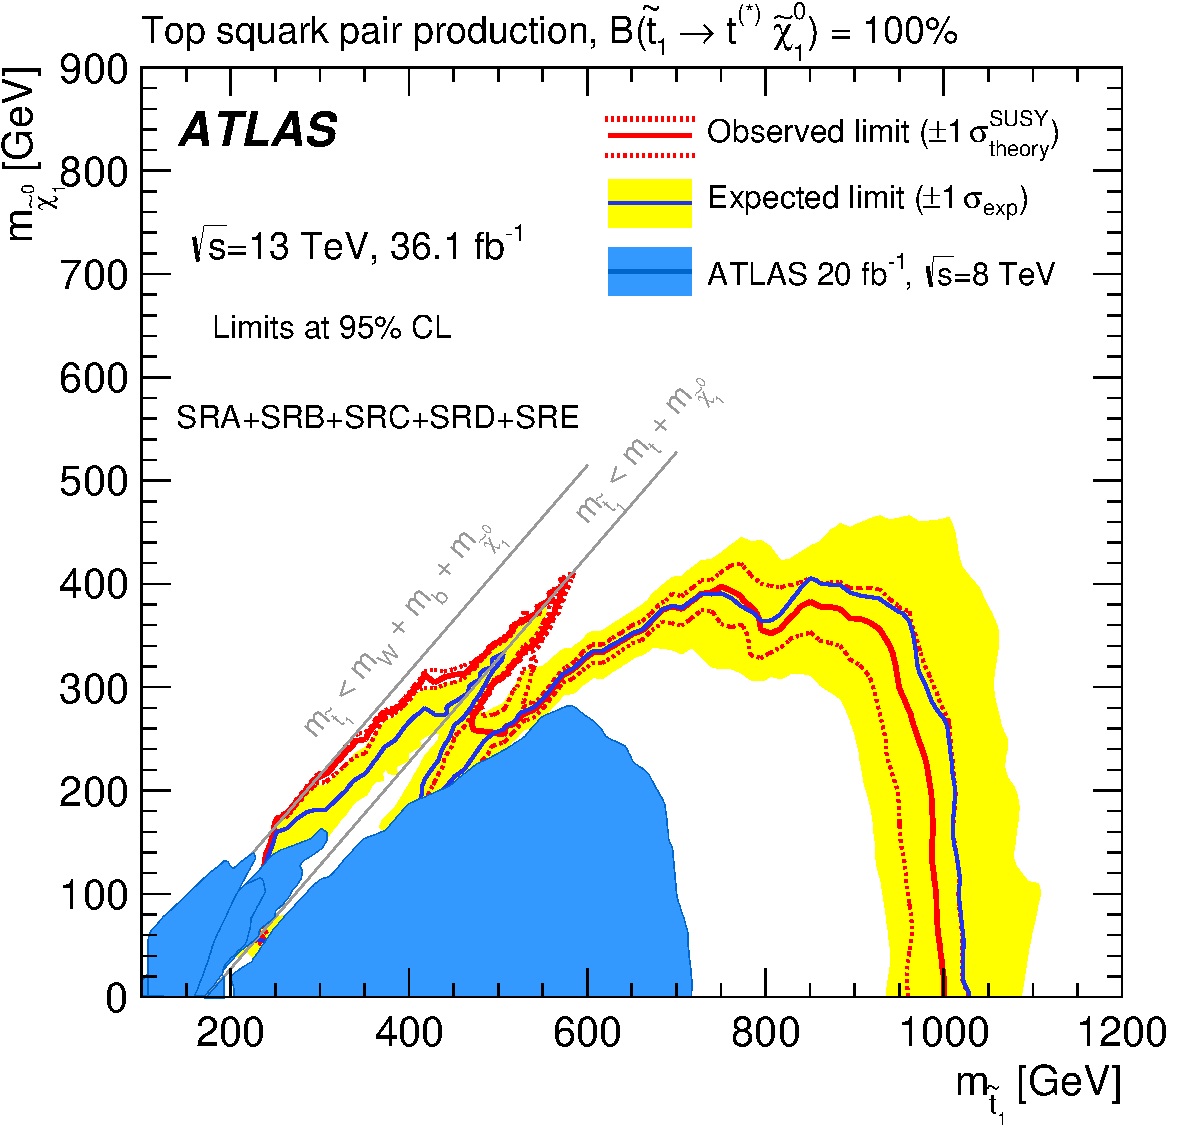
\includegraphics[width=0.7\textwidth]{stop/fit/atlascls_m0m12_wband1_showcms0_StopZL2016_SRABCDE}
			    \caption{Observed (red solid line) and expected (blue solid line)
			      exclusion contours at 95\% CL as a function of $\stop$ and
			      $\ninoone$ masses in the scenario where both top squarks decay
			      via $\stop\to t^{(*)} \ninoone$. Masses that are within the contours are excluded. Uncertainty bands corresponding to the $\pm 1
			      \sigma$ variation of the expected limit (yellow band) and the
			      sensitivity of the observed limit to $\pm 1\sigma$ variations of
			      the signal theoretical uncertainties (red dotted lines) are also
			      indicated~\cite{stop0L}. Observed limits from all third-generation Run-1 searches~\cite{Atlas8TeVSummary} at $\sqrt{s}=8$ TeV overlaid for comparison in blue (taken from~\cite{stop0L}).}
			    \label{fig:SRABC_exclusion}
			  \end{center}
			\end{figure}

			Signal models where top-squark decays into $b \chinoonepm$, or into additional massive neutralinos, are interpreted in four different scenarios~\cite{stop0L}:

			\begin{description}
			  \item[\boldmath Natural SUSY-inspired mixed grid:] this is a simplified model~\cite{Papucci2011} where $m_{\chinoonepm}=\mLSP+1\gev$ with two decay modes, $\stop\to b \chinoonepm$ and $\stop\to t\LSP$. Only on-shell top-quark decays are considered. The maximal mixing between the partners of the left- and right-handed top quarks, and the nature of the \LSP\ (pure bino) is assumed to be the same as for the $B$($\stop\to t\LSP$)=$100\%$ case. The branching ratio to $\stop\to t\LSP$ is set to $0\%$, $25\%$, $50\%$, and $75\%$. The limits obtained are shown in Figure~\ref{fig:tbMet_exclusion}~\cite{stop0L}).

				\item[\boldmath Non-asymptotic higgsino:] a simplified model inspired to the \ac{pMSSM} with a higgsino \ac{LSP}, ${m_{\chinoonepm}=\mLSP+5\gev}$, and ${m_{\ninotwo}=\mLSP+10\gev}$. This assumes three sets of branching ratios for the considered decays of $\stop\to t\ninotwo$, $\stop\to t\LSP$, $\stop\to b\chinoonepm$~\cite{Papucci2011}. In particular, a set of branching ratios with $B$($\stop\to t\ninotwo$, $\stop\to t\LSP$, $\stop\to b\chinoonepm$) = $33\%$, $33\%$, $33\%$, which is equivalent to a \ac{pMSSM} model with the lightest top squark mostly consisting of the superpartner of left-handed top quark and $\tanb=60$, is considered; and other two sets of branching ratios $B$($\stop\to t\ninotwo$, $\stop\to t\LSP$, $\stop\to b\chinoonepm$) = $45\%$, $10\%$, $45\%$ and $B$($\stop\to t\ninotwo$, $\stop\to t\LSP$, $\stop\to b\chinoonepm$) = $25\%$, $50\%$, $25\%$ are considered. These correspond to the scenarios in which $\mqlthree < \mtr$, independently of the choice of \tanb, and $\mtr<\mqlthree$ with $\tanb=20$, respectively. As mentioned in Chapter~\ref{ch:theory}, \mqlthree\ represents the left-handed third-generation mass parameter and \mtr\ is the mass parameter of the superpartner to the right-handed top quark. The limits for this interpretation are shown in Figure~\ref{fig:nonAsymhiggsino_exclusion} in the \mstop-\mLSP\ plane~\cite{stop0L}).

				\item[\boldmath Wino-NLSP pMSSM:] this is a \ac{pMSSM} model where the \ac{LSP} is bino-like with mass \mone\ and the \ac{NLSP} is wino-like with mass \mtwo, with $\mtwo=2\mone$ and $\mstop>\mone$~\cite{Papucci2011}. Limits (Figure~\ref{fig:winoNLSP_exclusion}) are set for both positive and negative higgsino mass parameter, $\mu$, as a function of the \stop\ and \ninoone\ masses which can be translated to different \mone\ and \mqlthree. In this interpretation only bottom- and top-squark production are considered. Furthermore, in this model the allowed decays in the top-squark production scenario are $\stop\to t \ninotwo\to h/Z \LSP$, with a maximum branching ratio of 33\%, and $\stop \to b \chinoonepm$. The $\ninotwo$ decay into either a $h$ or $Z$ is determined by the sign of $\mu$. In addition, the $\stop\to t\LSP$ decay with 100\% branching ratio is also considered along the diagonal region. The equivalent decays in bottom-squark production are $\sbottom\to t\chinoonepm$ and $\sbottom\to b\ninotwo$~\cite{stop0L}). %The remaining \ac{pMSSM} parameters have the following values: $\mthree=2.2$ TeV (gluino mass parameter), $\ms=\sqrt{m_{\stopone} m_{\stoptwo}}=1.2$ TeV (geometric mean of top-squark masses), $\xtms=\sqrt{6}$ (mixing parameter between the superpartners of left- and right-handed states, where $X_{t}=\at-\mu/\tanb$ and $\at$ is the trilinear coupling parameter in the top-quark sector), and $\tanb=20$. All other \ac{pMSSM} masses are set to $>3$ \TeV.

				\item[\boldmath Well-tempered neutralino pMSSM:] in this \ac{pMSSM} model three light neutralinos and a light chargino (mixtures of bino and higgsino states), are considered with masses within $50$~\GeV\ of the lightest state~\cite{atlasDM,wellTemp}. Such model is designed to satisfy the \ac{SM} Higgs boson mass and the dark-matter relic density ($0.10<\Omega h^{2}<0.12$, where $\Omega$ is energy density parameter and $h$ is the Planck constant~\cite{relic_density}).
				 %with \ac{pMSSM} parameters: $\mone=-(\mu+\delta)$ where $\delta=20$--$50\gev$, $\mtwo=2.0$ TeV, $\mthree=1.8$ TeV, $\ms=0.8$--$1.2$~\TeV, $\xtms\sim\sqrt{6}$, and $\tanb=20$. 
				The limits for this model are shown in Figure~\ref{fig:wellTemp_exclusion}. In this interpretation only bottom- and top-squark production are considered. Furthermore, the signal grid points were produced in two planes, $\mu$-\mtr\ and $\mu$-\mqlthree, and then projected to the corresponding \stop\ and \ninoone\ masses~\cite{stop0L}).% The remaining \ac{pMSSM} masses are set to $>3$ TeV.
			\end{description}

			\begin{figure}[htpb]
			  \begin{center}
			    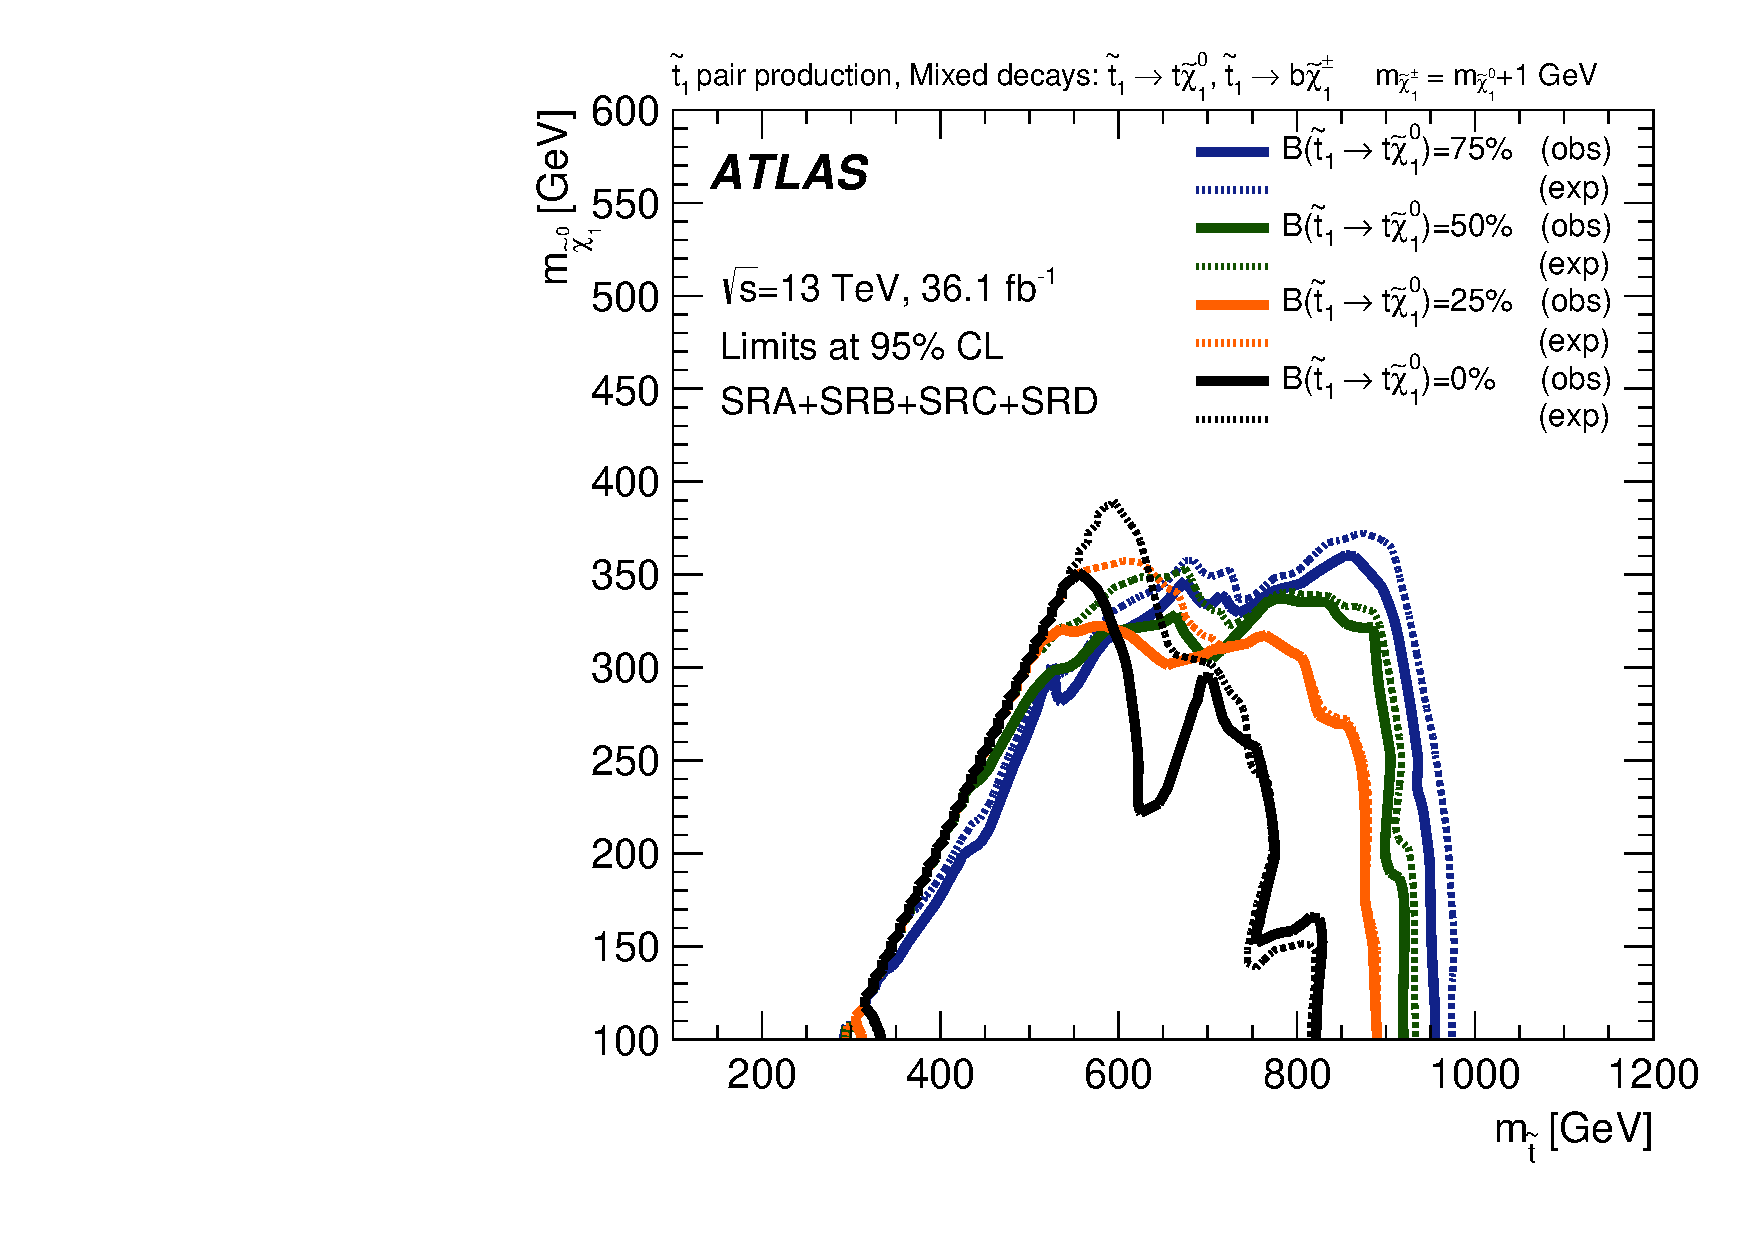
\includegraphics[width=0.7\textwidth]{figures/fit/SRABCD_mixed_dm1}
			    \caption{Observed (solid line) and expected (dashed line) exclusion contours at 95\% CL as a function of $\stop$ and $\ninoone$ masses and branching ratio to $\stop\to t\LSP$ in the natural SUSY-inspired mixed grid scenario where $m_{\chinoonepm}=\mLSP+1\gev$ (taken from~\cite{stop0L}).}
			    \label{fig:tbMet_exclusion}
			  \end{center}
			\end{figure}

			\begin{figure}[htpb]
			  \begin{center}
			   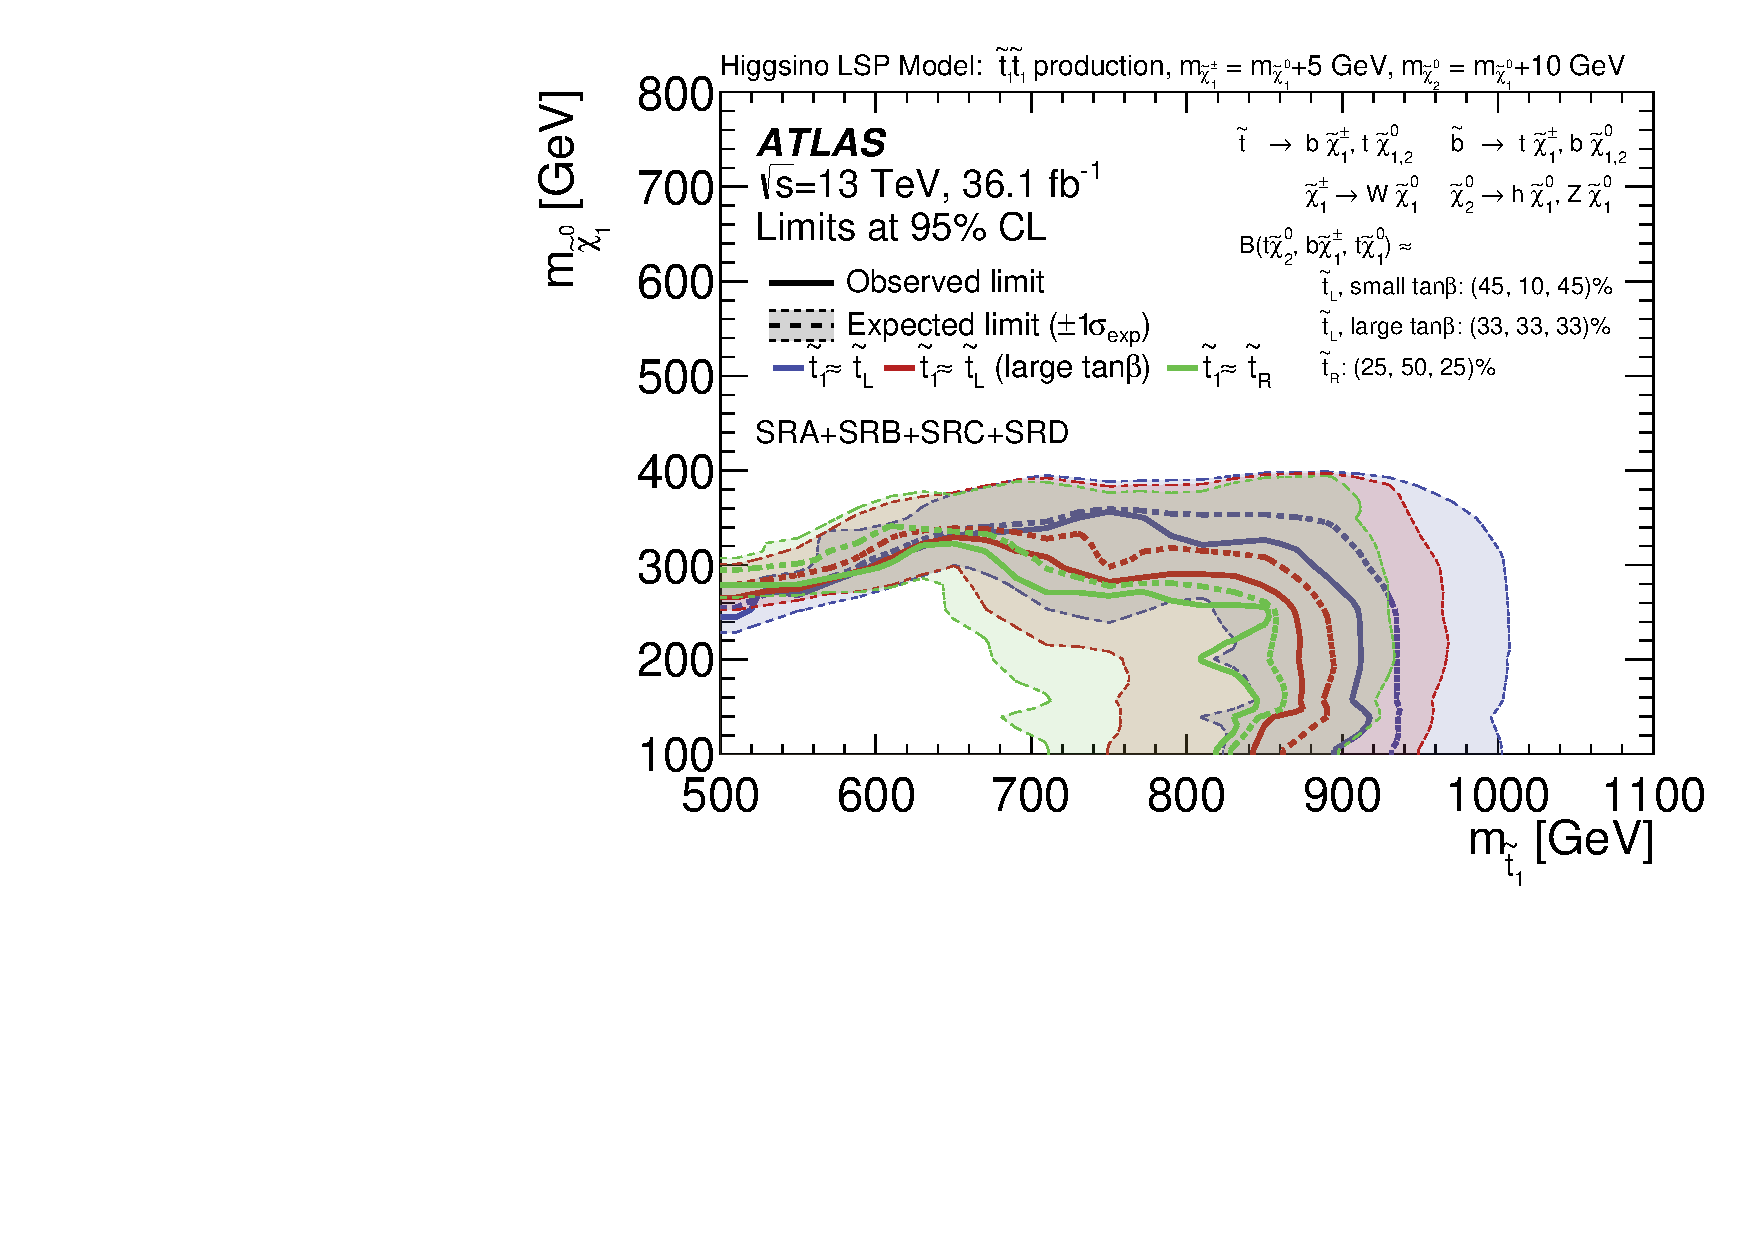
\includegraphics[width=0.7\textwidth]{figures/fit/SRABCD_tN1tN2bC1.pdf}
			    \caption{Observed (solid line) and expected (dashed line) exclusion contours at 95\% CL as a function of \mstop\ and \mLSP\ for the pMSSM-inspired non-asymptotic higgsino simplified model for a small tan$\beta$ with $B$($\stop\to t\ninotwo$, $\stop\to t\LSP$, $\stop\to b\chinoonepm$) = 45\%, 10\%, 45\% (blue), a large tan$\beta$ with $B$($\stop\to t\ninotwo$, $\stop\to t\LSP$, $\stop\to b\chinoonepm$) = 33\%, 33\%, 33\% (red), and a small $\tilde t_{R}$ with $B$($\stop\to t\ninotwo$, $\stop\to t\LSP$, $\stop\to b\chinoonepm$) = 25\%, 50\%, 25\% (green) assumption. Uncertainty bands correspond to the $\pm 1 \sigma$ variation of the expected limit(taken from~\cite{stop0L}).}
			    \label{fig:nonAsymhiggsino_exclusion}
			  \end{center}
			\end{figure}

			\begin{figure}[htpb]
			  \begin{center}
			    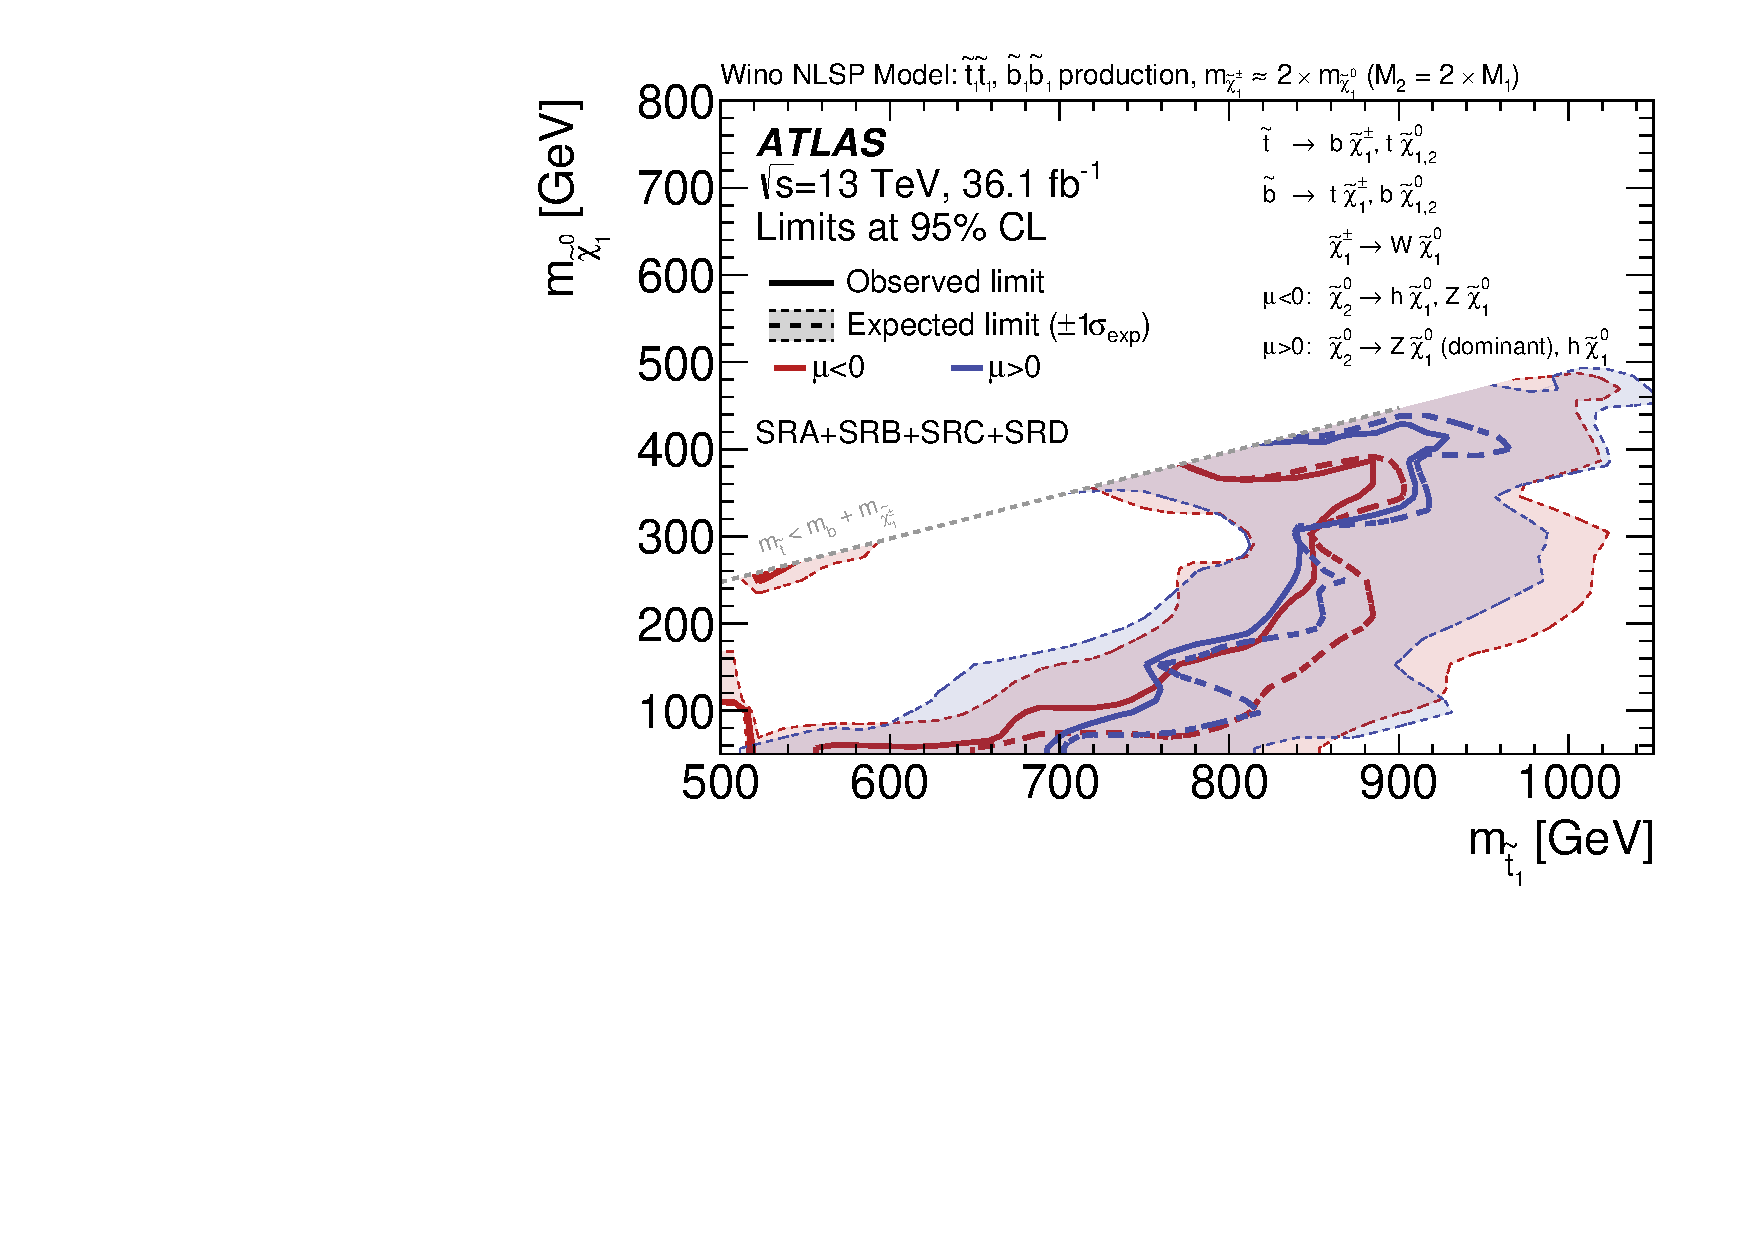
\includegraphics[width=0.7\textwidth]{figures/fit/SRABCD_winoNLSP.pdf}
			    \caption{Observed (solid line) and expected (dashed line) exclusion contours at 95\% CL as a function of $\stop$ and $\ninoone$ masses for the Wino NLSP pMSSM model for both positive (blue) and negative (red) values of $\mu$. Uncertainty bands correspond to the $\pm 1 \sigma$ variation of the expected limit (taken from~\cite{stop0L}).}
			    \label{fig:winoNLSP_exclusion}
			  \end{center}
			\end{figure}

			\begin{figure}[htpb]
			  \begin{center}
			    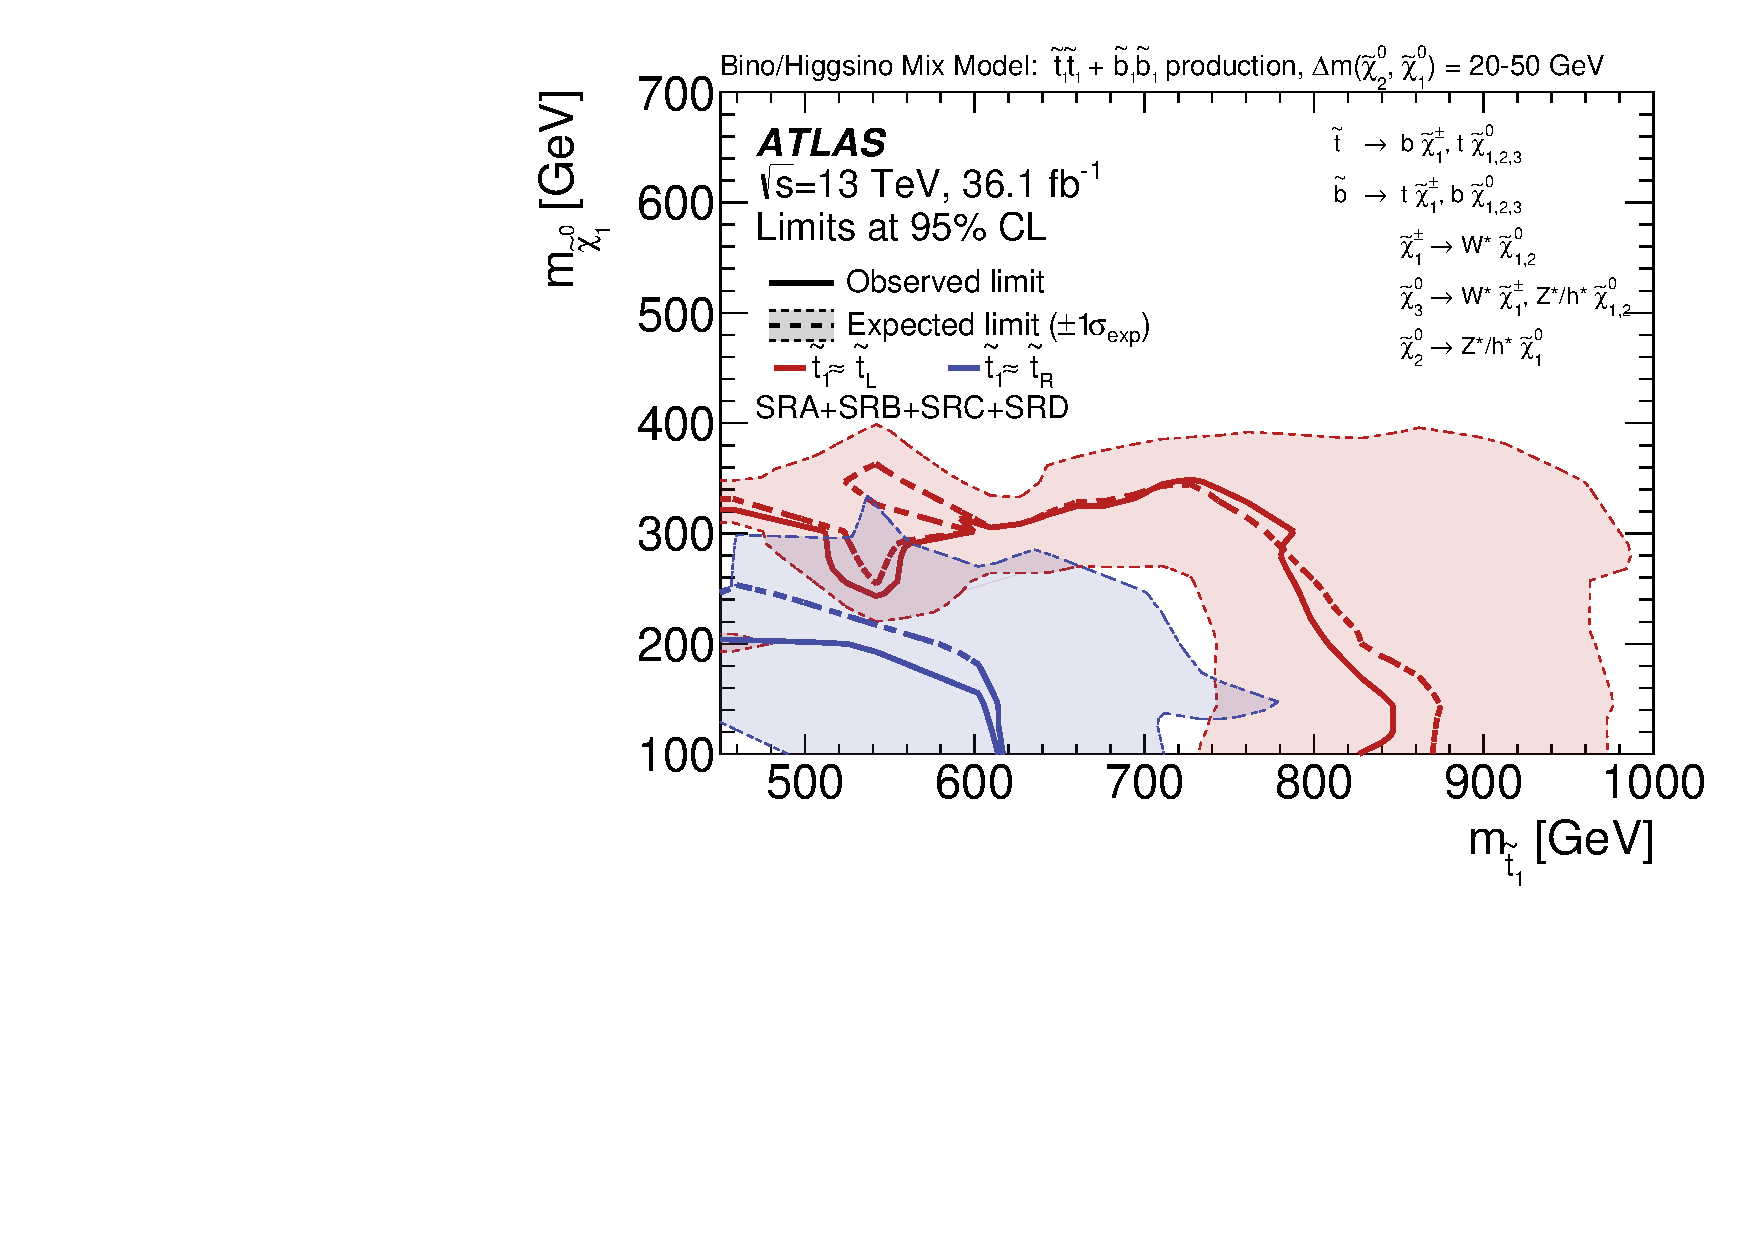
\includegraphics[width=0.7\textwidth]{figures/fit/SRABCD_wellTempered.pdf}
			    \caption{Observed (solid line) and expected (dashed line) exclusion contours at 95\% CL as a function of $\stop$ and $\ninoone$ masses for the $\tilde t_{L}$ scan (red) as well as for the $\tilde t_{R}$ scan (blue) in the well-tempered pMSSM model. Uncertainty bands correspond to the $\pm 1 \sigma$ variation of the expected limit (taken from~\cite{stop0L}).} 
			    \label{fig:wellTemp_exclusion}
			  \end{center}
			\end{figure}

			Finally, the results for SRE are interpreted for gluino-mediated top-squark production via gluino decays in terms of the \stop-$\gluino$ mass plane with $\Delta m(\stop,\ninoone)=5\GeV$. Figure~\ref{fig:SRE_exclusion} shows the exclusion plot of gluino masses up to $m_{\gluino}=1800\GeV$ with $\mstop<800\GeV$~\cite{stop0L}).

			\begin{figure}[htpb]
			  \begin{center}
			    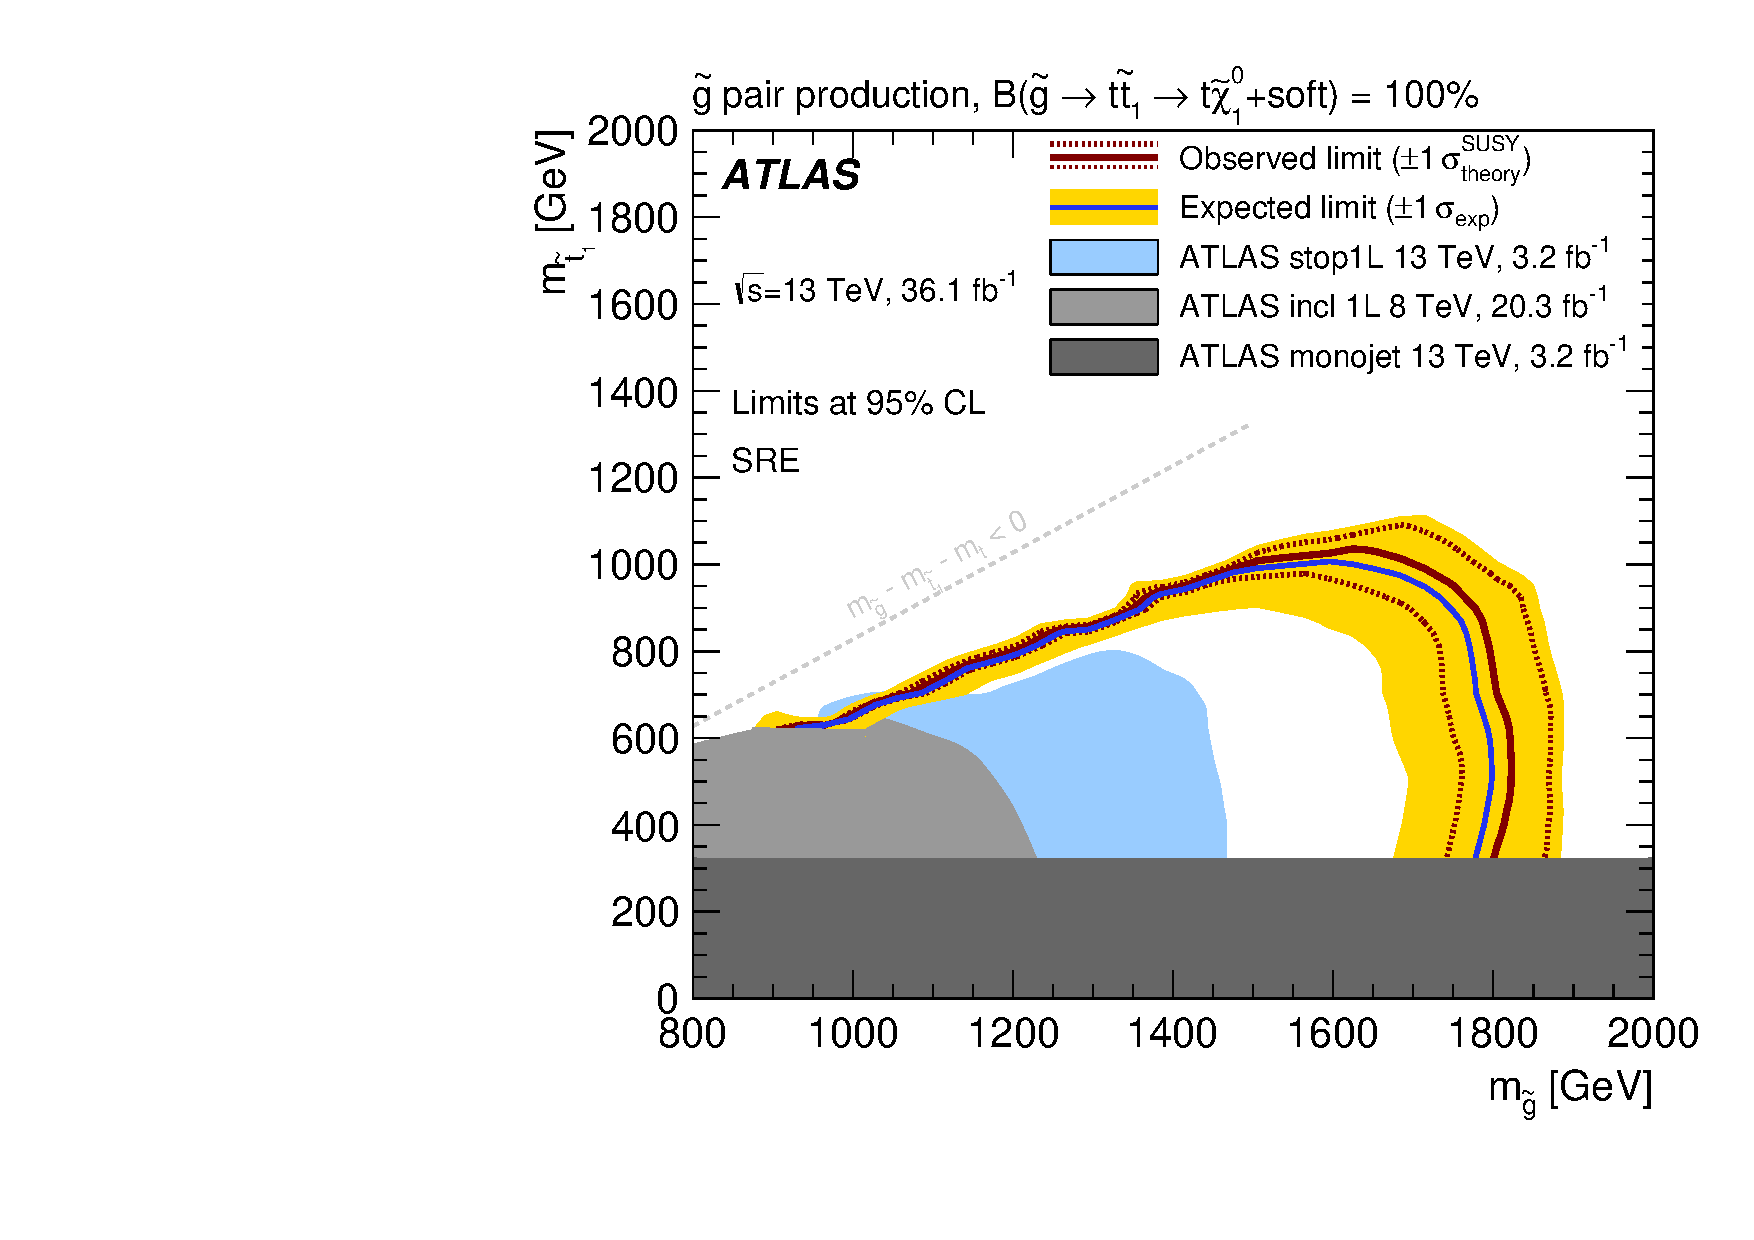
\includegraphics[width=0.7\textwidth]{figures/fit/SRE_exclusion}
			    \caption{Observed (red solid line) and expected (blue solid line)
			      exclusion contours at 95\% CL as a function
			      of $\gluino$ and $\stop$ masses in the scenario where both
			      gluinos decay via $\gluino\to t\stop\to t\ninoone+$soft
			      and $\Delta m(\stop,\ninoone)=5\GeV$. Uncertainty bands corresponding to the $\pm 1
			      \sigma$ variation of the expected limit (yellow band) and the
			      sensitivity of the observed limit to $\pm 1\sigma$ variations of
			      the signal theoretical uncertainties (red dotted lines) are also
			      indicated. Observed limits from previous searches with the ATLAS detector at $\sqrt{s}=8$ and $\sqrt{s}=13$ TeV are overlaid in grey and blue~\cite{stop1L,Gtc1L,GtcMonojet} (taken from~\cite{stop0L}).}
			    \label{fig:SRE_exclusion}
			  \end{center}
			\end{figure}

        % \chapter*{Conclusion}
\addcontentsline{toc}{chapter}{Conclusion}
\markboth{}{Conclusion}

Last thing to write


    %---------------------------------------------------
    % THESIS CONTENT - APPENDICES
    %---------------------------------------------------
    \backmatter
        \appendix
        \chapter{\ttZ\ estimation for a Dark Matter search}
\markboth{}{Appendix A}
\label{app:ttzdm}

	The data-driven background estimation technique, already discussed in Section~\ref{sec:ddbkgest}, and the theory uncertainties calculation prescription presented in Section~\ref{sec:syst_unc}, were also used in the search for dark matter produced in association with third-generation quarks, which was published in October $2017$ in the \EPJ~\cite{DMhf}. The author's contribution to this analysis only regarded the \ttZ\ background estimation and the computation of the relevant theory uncertainties and, as such, only these two topics will be hereby covered.


	\section{Overview of the analysis}

		\begin{table}[!htb]
			\caption{Summary of the kinematic and topology-dependent selections for signal regions SRt1 and SRt2~\cite{DMhf}. SRt3 is not reported as it was not relevant for the estimation of the \ttZ\ background.}
			\centering
			\renewcommand{\arraystretch}{1.5}
				\begin{tabular}{lcc}
					\toprule
					\textbf{Observable}  & \textbf{SRt1} & \textbf{SRt2} \\
					\midrule
					Trigger             &   \multicolumn{2}{c}{\met}   \\
					\antikt\ $R=0.4$ jets  & \multicolumn{2}{c}{$\ge 4,~\pt>80,80,40,40 \gev$} \\
					$N_{\bjs}$  & \multicolumn{2}{c}{$\geq2$} \\[0.3ex]
					$N_{\ell}$  & \multicolumn{2}{c}{$0$} \\[0.3ex]
					\midrule
					\met\ [\GeV]         &\multicolumn{2}{c}{$>300$}  \\
					$\pt$ leading \bj\ [\GeV] &  \multicolumn{2}{c}{$>20$}   \\
					\midrule
					\mantikteightzero\ [\GeV] & $>80$ & -     \\
					\mantikteightone\ [\GeV] & $>80$ & -     \\
					\mtbmin\ [\GeV]           & $>150$ & $>200$ \\
					\mtbmax\ [\GeV]           & $>250$ & -      \\
					\drbb\    & \multicolumn{2}{c}{$>1.5$} \\
					\metsig\  [$\sqrt{\GeV}$] & - & $>12$ \\
					\midrule
					%\multicolumn{3}{l}{Multi-jet rejection specific} \\
					\dphimin\ [rad]     &  \multicolumn{2}{c}{$>0.4$} \\
					\mettrack [\GeV]   &  \multicolumn{2}{c}{$> 30$}  \\
					$\Delta\phi(\ptmiss,\ptmisstrk)$  [rad] & \multicolumn{2}{c}{$< \pi/3$} \\
					\bottomrule
				\end{tabular}
			\label{tab:srtselections}
		\end{table}

		\begin{wrapfigure}{R}{.33\textwidth}
			\centering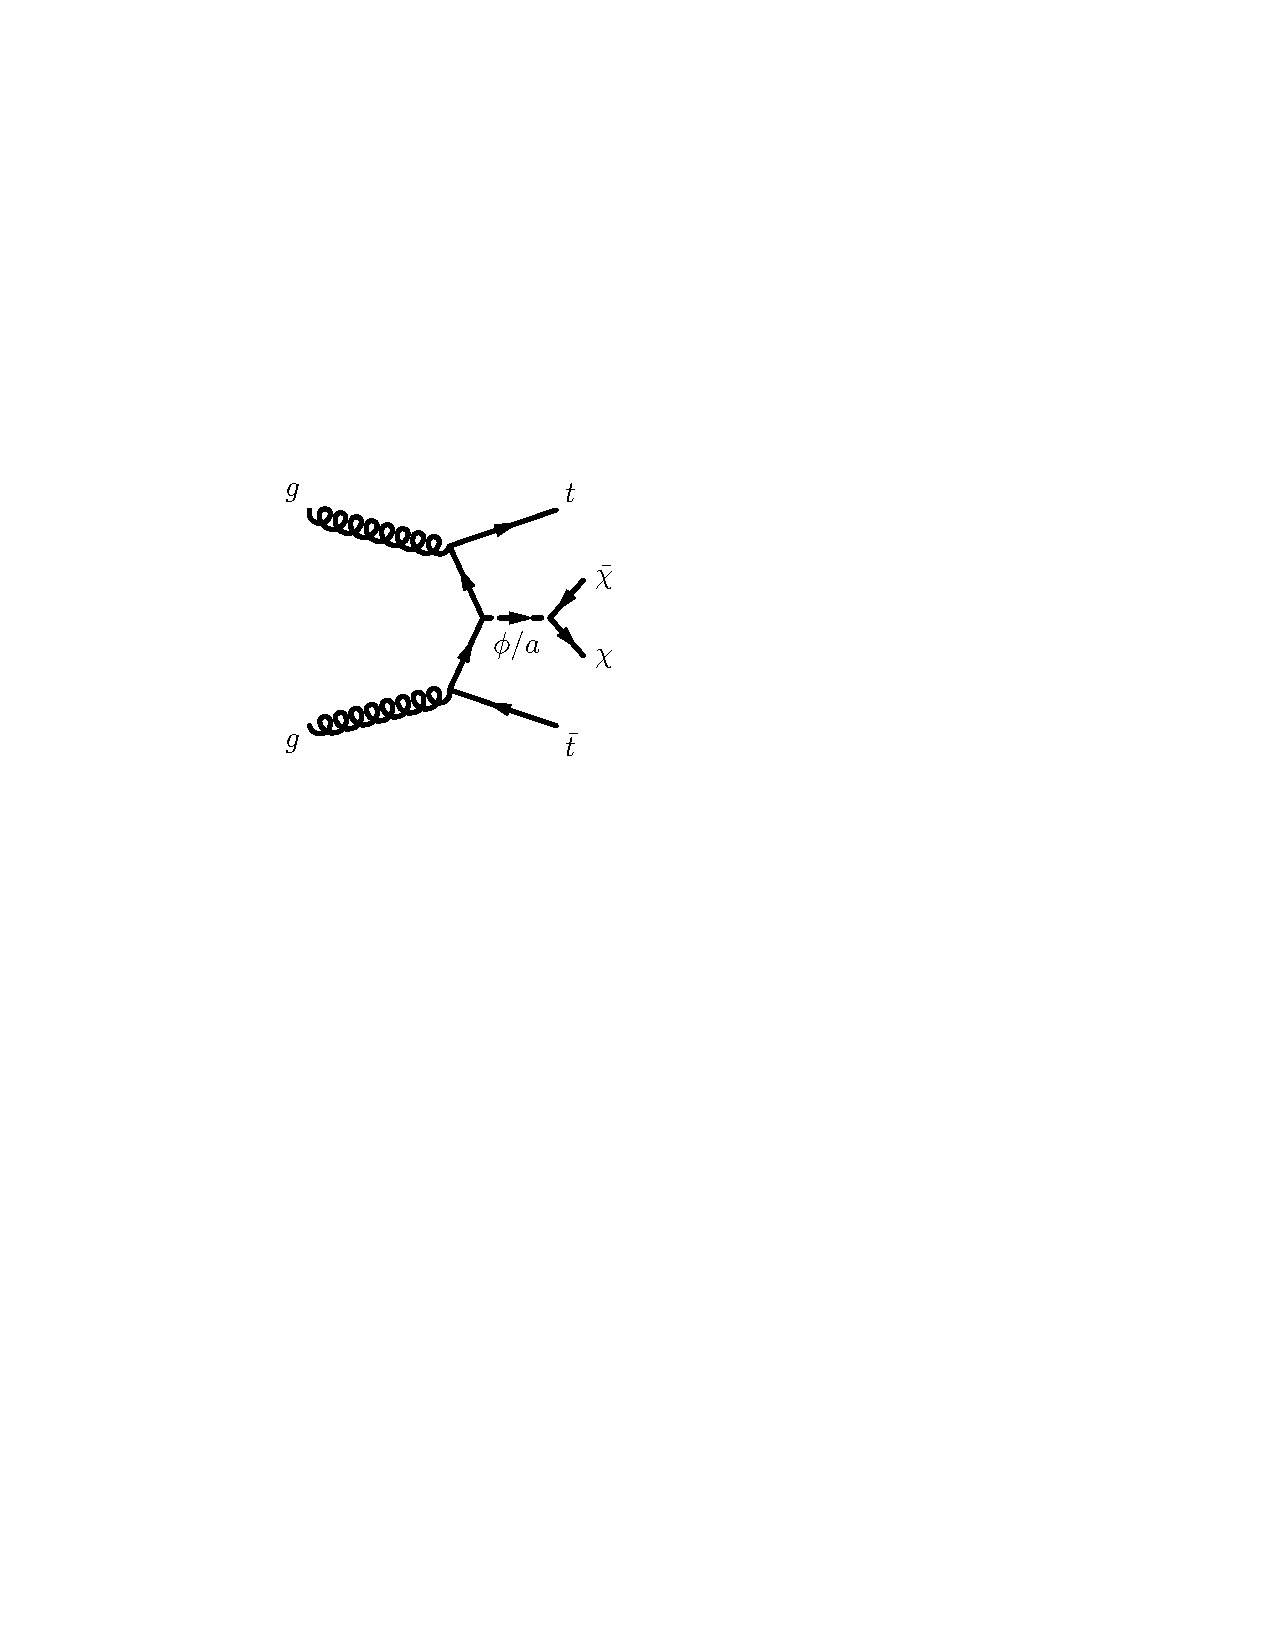
\includegraphics[width=.3\textwidth]{appA/TTphi}
			\caption{Representative diagram at the lowest order for spin-0 mediator associated production with top quarks $\ttbar+\phi/a$ (taken from~\cite{DMhf}).}
			\label{fig:dmhfModels}
		\end{wrapfigure}

		The analysis also used $36.1\, \ifb$ of \pp\ collisions delivered by the \ac{LHC} and recorded with the \ac{ATLAS} detector, and it targeted final states with either bottom- or top-quark pairs and missing transverse momentum. In particular, only the final state with two top quarks and missing transverse momentum, as shown in Figure~\ref{fig:dmhfModels}, will be considered here. The $0\ell$ final state of this analysis essentially yields an experimental signature identical to the one discussed in Chapter~\ref{ch:stop_ana}, namely 4 or more jets, two of which $b$-tagged, and missing transverse momentum. For such reason, the physics objects used in this analysis, and the variables employed for the design of a \ttgamma\ \ac{CR} to estimate the \ttZ\ background, are the same as those already extensively discussed in Chapters~\ref{ch:stop_ana}, and~\ref{ch:bkgest}. 

		Five \acp{SR} are employed in this analysis: SRb1, SRb2, SRt1, SRt2, and SRt3. SRb1 and SRb2 are optimised for models in which \ac{DM} is produced in association with one or two $b$-quarks and these will not be further considered as the author did not contribute to this part of the analysis. SRt1, SRt2, and SRt3, are optimised to isolate events in which \ac{DM} is produced in association with a top-antitop pair, that either decays fully hadronically (SRt1 and SRt2) or dileptonically (SRt3)~\cite{DMhf}. While the $\ttZ(\to \nu\bar{\nu})$ is an irreducible background in SRt1 and SRt2, it is negligible in SRt3 and therefore such \ac{SR} will be neglected here. SRt1 and SRt2 have a very similar background composition as the one discussed in Chapter~\ref{ch:stop_ana} and they target low ($< 100$ \GeV) and high (between $100$ and $350$ \GeV) mediator mass assumptions, respectively. 
		%The two \acp{SR} have selections criteria which overlap. 
		%As the \ac{SR} optimisation strategy of this analysis did not affect the \ttZ\ background estimation, the design of such \acp{SR} will not be further discussed, although the \acp{SR}, where 
		Table~\ref{tab:srtselections} shows the SRt1 and SRt2 selections.% where the \ttZ\ background estimation was employed. 


	\section{The estimation of the irreducible \ttZ\ background}

		\begin{table}[!htb]
			\parbox{.5\linewidth}{
			\centering
			\captionof{table}{Summary of the CR$\gamma$ selection for the \ttZ\ background estimation.}\label{tab:CRcuts}
		   	\begin{tabular}{lc}
					\toprule
					\textbf{Observable} & \textbf{CR}\boldmath{$\gamma$} \\
					\midrule
					Trigger & photon\\
					$N_{\mathrm{jets}}$ & $\geq 4$ \\ 
					$N_{\bjs}$ & $\geq 2$ \\ \midrule
					$N_\gamma$ & $1$ \\ 
					$\pt^{\gamma}$ [\GeV] & $>150$ \\
					$N_\ell$ & $1$ \\ 
					$\pt(\ell_1)$ [\GeV] & $>28$ \\ \bottomrule
			  \end{tabular}
			}
			\hfill
			\parbox{.5\linewidth}{
			\centering
			\captionof{table}{Background composition of \ttgamma\ CR. Pre-fit yields, statistical and detector systematic uncertainties shown.}
			\label{tab:CRgamma_yields}
				\begin{tabular}{lc}
					\toprule
					\textbf{Process} & \textbf{Yield} \\
					\toprule
					\ttgamma & $89.50 \pm 2.02$ \\
					$V+\gamma$ & $5.01 \pm 1.12$ \\
					$\ttbar$ & $4.26 \pm 0.94$ \\
					$\ttV$ & $1.79 \pm 0.23$ \\
					single Top & $1.86 \pm 0.52$ \\
					$Z$ & $0.56 \pm 0.13$ \\
					$W$ & $0.03 \pm 0.01$ \\
					\midrule
					Total MC & $103.01 \pm 2.69$ \\
					Data & $124$ \\
					\midrule
					\multicolumn{2}{c}{\textbf{CR}{\bm{$\gamma$} purity} ( $87\%$)} \\ 
					\midrule
					$\mu_{\ttgamma}$ & $1.22 \pm 0.13$ \\
					\bottomrule
				\end{tabular}
			}
		\end{table}

		As in the $\tilde{t}0\ell$ analysis - the search for top squarks in all-hadronic final states presented in Chapters~\ref{ch:stop_ana},~\ref{ch:bkgest}, and~\ref{ch:results} - the \ttV\ events, and in particular \ttZ\ events where the $Z$ boson decays into neutrinos, represent an irreducible background for the \acp{SR} targeting dark matter produced in association with top quarks (Figure~\ref{fig:dmhfModels}). Once again, a data-driven approach is employed to estimate such background. In particular, events with $\pt^{\gamma} > m_{\mathrm Z}$, resembling $\ttZ( \to \nu\bar{\nu})$ ones, are selected. The CR${\gamma}$ selection, detailed in Table~\ref{tab:CRcuts}, allows to select events with exactly one energetic tight photon and at least one lepton from the decay of the \ttbar\ system. Such \ac{CR} essentially is identical to the one in Table~\ref{tab:CRTTGamma} already shown in Section~\ref{sec:ddbkgest} (page \pageref{sec:ddbkgest}), except for the applied trigger which is a single-photon instead of a single-lepton trigger. This strategy was found to allow the \ac{CR} CR$\gamma$ to better mimic the hard kinematic requirements of the two \acp{SR} targeting the signal in Figure~\ref{fig:dmhfModels}~\cite{DMhf}. Finally, in order to mimic the expected missing transverse momentum spectrum of $Z\rightarrow\nu\bar{\nu}$ events, the \pt\ of the photon $\left ( \pt^{\gamma} \right )$ is vectorially added to the \ptmiss, to form a variable called \metprimeg.



	\section{Results}

		A normalisation factor for the \ttZ\ \ac{SM} background, $\mu_{\ttZ} = 1.22$, was obtained by performing the background-only fit - employing the same procedure discussed in Chapter~\ref{ch:results} - including all the \ac{SM} backgrounds. Figure~\ref{fig:metprimecrgamma} shows the distribution of \metprimeg\ in CR$\gamma$ where a very good data/MC agreement was found. Lastly, by employing the same procedure discussed in Section~\ref{sec:syst_unc} the theory uncertainties were computed and found to be between $6\%-10\%$ across the various \acp{SR}. Additionally, Table~\ref{tab:CRgamma_yields} shows the background composition of CR$\gamma$, where an $87\%$ purity was reached.

		\begin{figure}[!htb]
		\centering
			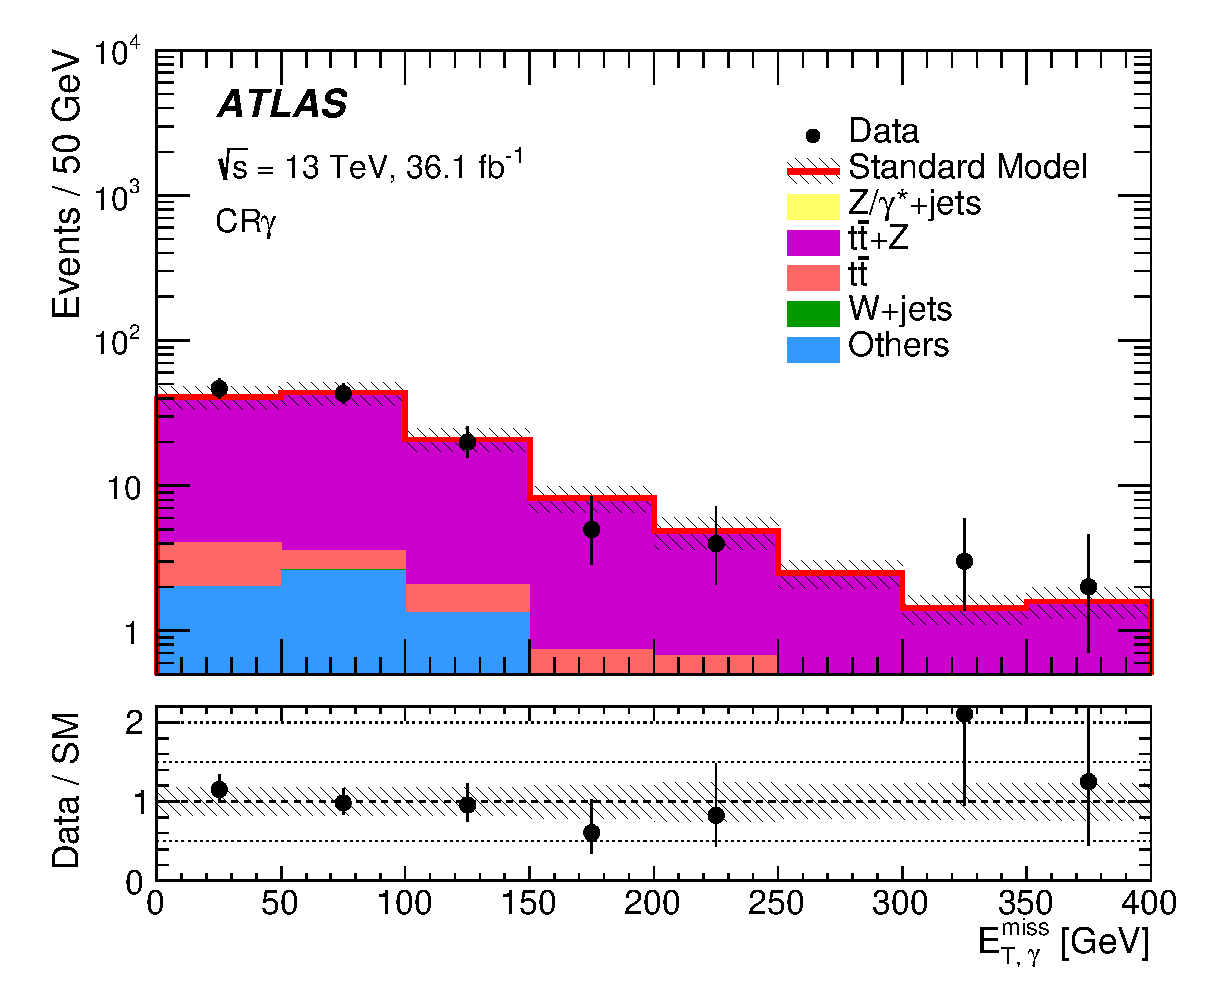
\includegraphics[width=.8\textwidth]{appA/can_CRttG_MetTST_met_afterFit}
			\caption{Comparison of the data with the post-fit Monte Carlo prediction of the \metprimeg\ distribution in CR$\gamma$. The bottom panel shows the ratio of the data to the \ac{MC} prediction. The band includes all systematic
			detector-related and theory uncertainties. The last bins include overflows, where applicable (taken from~\cite{DMhf}).}
			\label{fig:metprimecrgamma}
		\end{figure}

		The data is found to be compatible with the background predictions in each one of the \acp{SR}. In particular, in each \ac{SR} the observed yields in data are above the expected background but within $1.3$ standard deviations of its uncertainty, too low to suggest the presence of any of the searched signal. A model-independent fit~\cite{histfitter}, where both \acp{CR} and \acp{SR} are included, is employed to derive $95\%$ \ac{CL} upper limits on the visible cross-section of new \ac{BSM} processes, defined as cross-section times acceptance times efficiency ($\langle\sigma A \epsilon\rangle_{\mathrm obs}^{95}$) and obtained as the upper limit on the number of BSM events divided by the total integrated luminosity. No systematic uncertainties for the signal are assumed for such limits and any possible signal contamination in the \acp{CR} is neglected. %The results are also used to set limits on the production cross-section of colour-neutral and colour-charged mediator models decaying into dark-matter particles. When deriving model-dependent limits, the expected signal yield in each fit region is considered. 

		Figures~\ref{fig:dmresults} and~\ref{fig:dmresultschi} show upper limits at 95\% CL on $\sigma / \sigma (g = 1.0)$, namely the signal cross-section scaled to the signal cross-section for coupling $g = 1$. To derive the results for the fully hadronic \ttbar\ final state the region SRt1 or SRt2 with the best expected sensitivity is used. The SRt1 was originally optimised for low-mass scalar mediators, while SRt2 was optimised for high-mass scalar mediators and pseudoscalar mediators. However, SRt1 is strongly affected by systematic uncertainties in the \ttbar\ modelling and therefore SRt2 sets more stringent limits for the whole parameter space. These limits are obtained both as a function of the mediator mass, assuming a specific \ac{DM} mass of $1$ \GeV\ (Figure~\ref{fig:dmresults}), and as a function of the \ac{DM} mass, assuming a specific mediator mass of $10$ \GeV\ (Figure~\ref{fig:dmresultschi}). Both the scalar and pseudoscalar mediator cases are considered. The sensitivity for $\ttbar + \phi/a$ on-shell decays is approximately constant for masses below $100$ \GeV, with SRt3 excluding the $g = 1$ assumption for scalar mediator masses up to $50$ \GeV. For a given mediator mass the acceptance of the analysis is independent of the value of the \ac{DM} mass as long as $m(\phi / a) > 2  m(\chi)$ is fulfilled. Under these conditions, exclusion limits for \ac{DM} masses differing from the one presented can be inferred from the result shown in Figure~\ref{fig:dmresults}. Due to the smaller Yukawa enhancement of $\bbbar + \phi / a$ final states, it is possible to exclude cross-sections $300$ times the nominal values for $g = 1$.


		\begin{figure}[!htb]
			\centering
			\subbottom[]{
				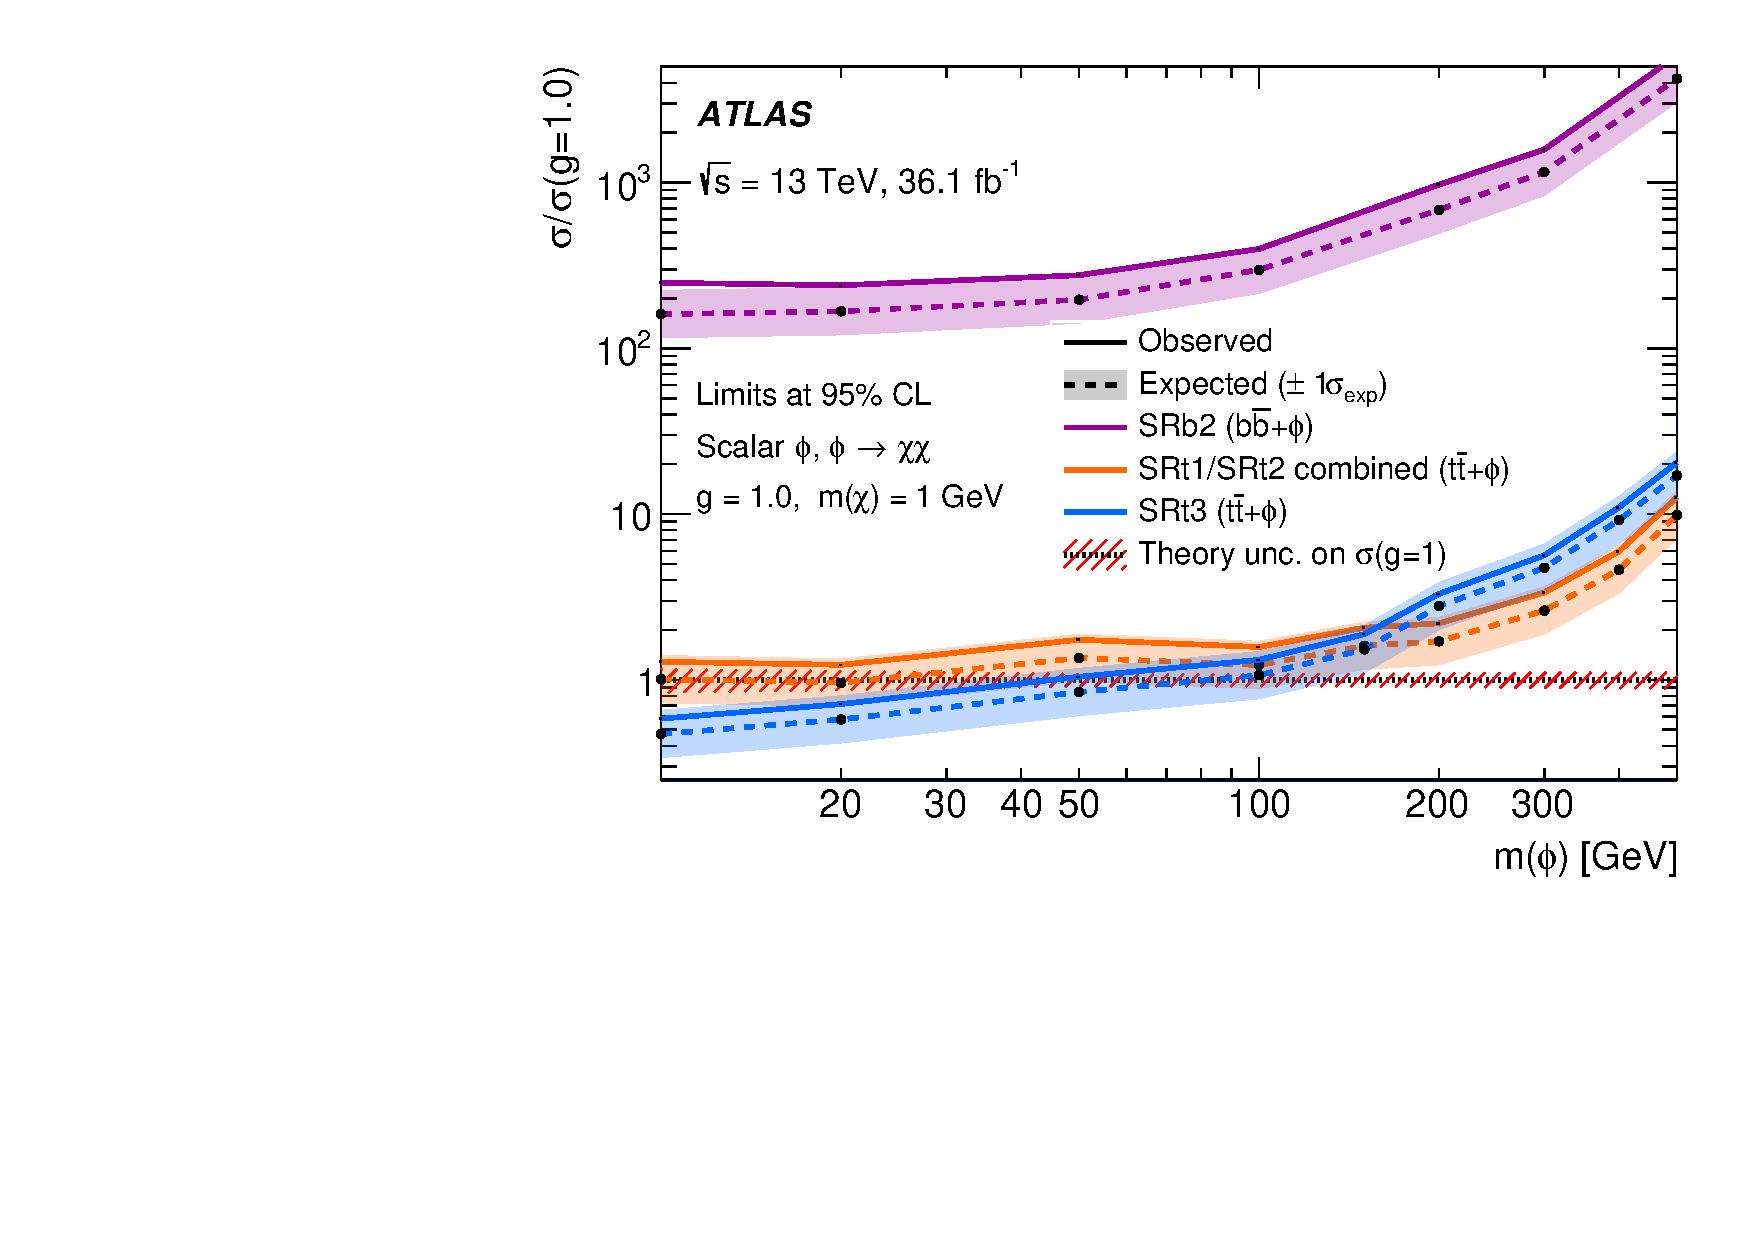
\includegraphics[width=.9\textwidth]{appA/final_scalar_SR1}}\\
			\subbottom[]{
				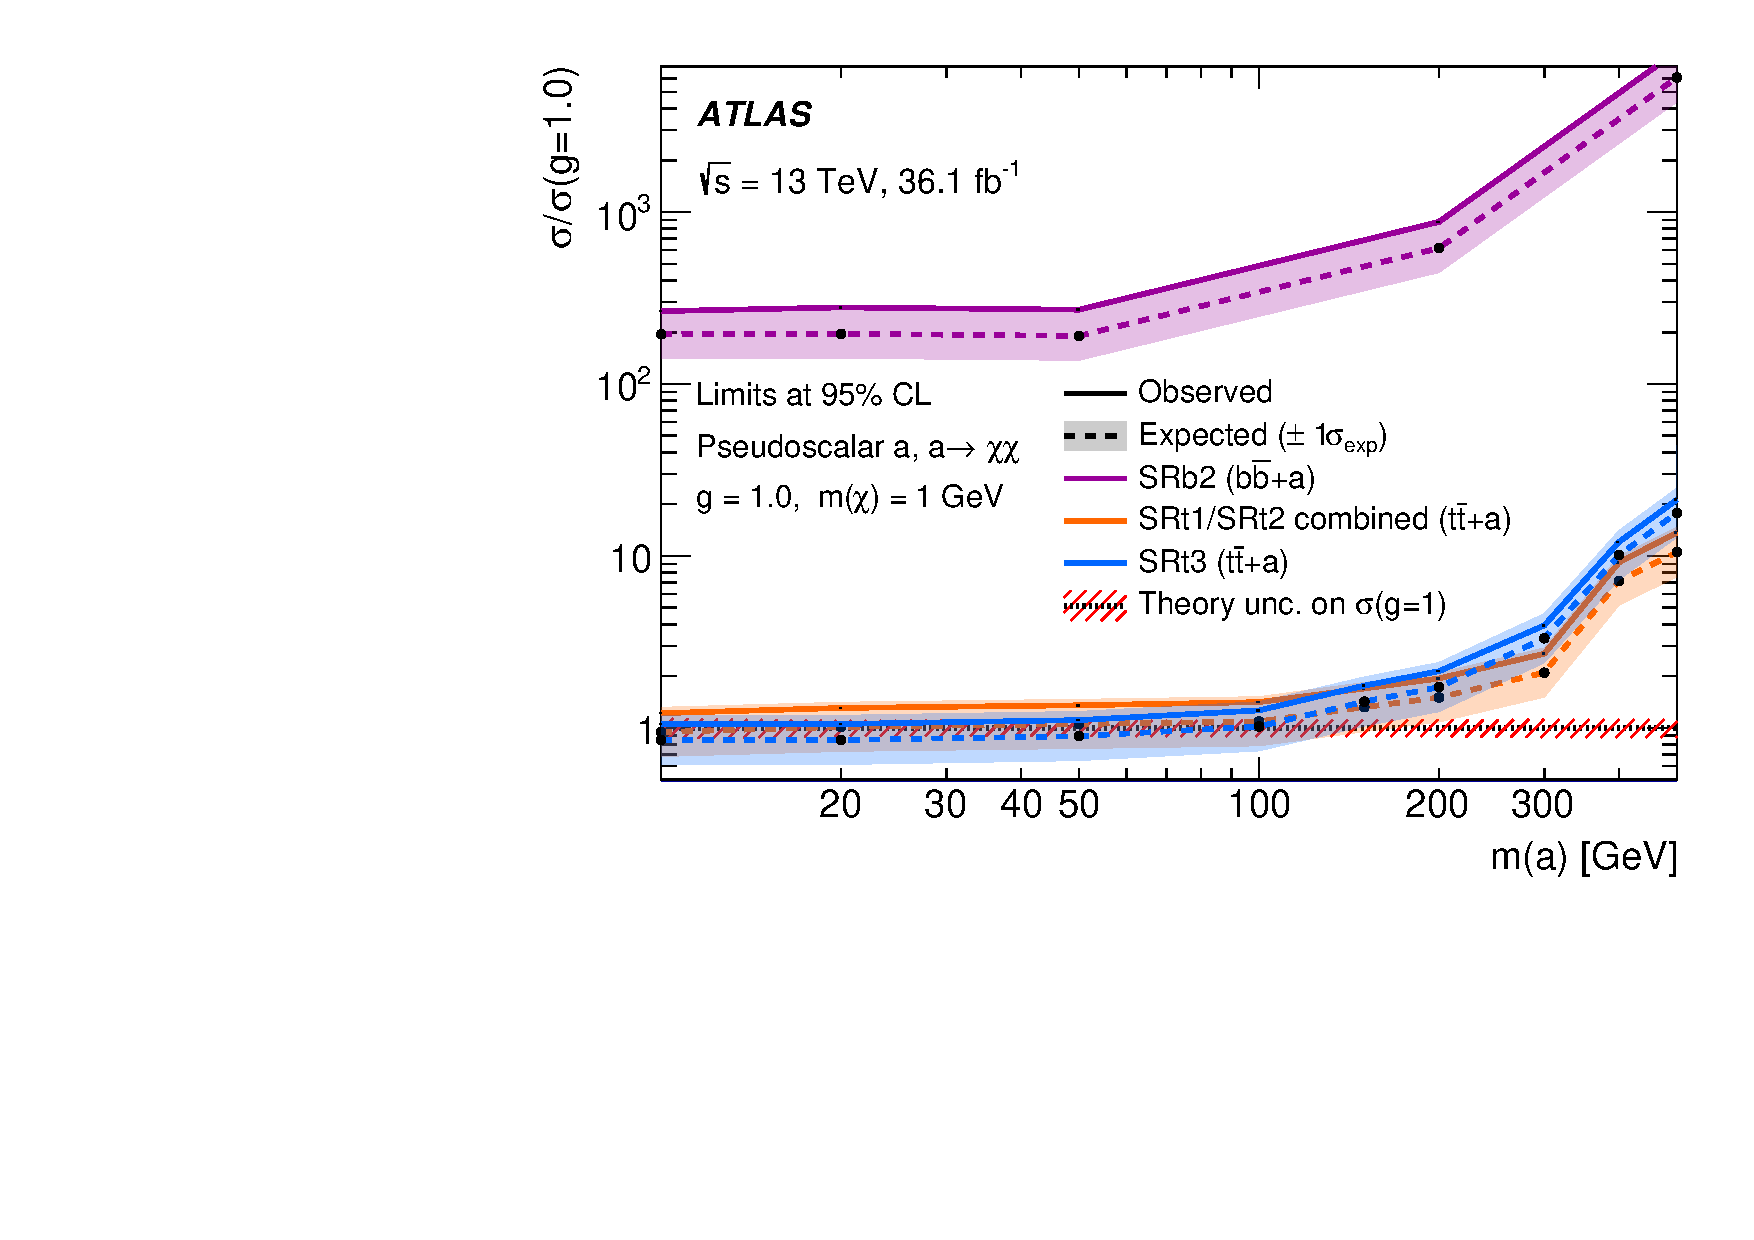
\includegraphics[width=.9\textwidth]{appA/final_pseudo_SR1}}
			\caption{Exclusion limits for colour-neutral $\ttbar/\bbbar+\phi$ scalar (a) and $\ttbar/\bbbar+a$ pseudoscalar (b) models as a function of the mediator mass for a DM mass of $1\;\GeV$. The limits are calculated at 95\% CL and are expressed in terms of the ratio of the excluded cross-section to the nominal cross-section for a coupling assumption of $g = g_q = g_\chi = 1$, where $g_\chi$ is the DM–mediator coupling, and $g_q$ the flavour-universal SM–mediator coupling. The solid (dashed) lines shows the observed (expected) exclusion limits for the different signal regions, according to the colour code specified in the legend. To derive the results for the fully hadronic \ttbar\ final state the region SRt1 or SRt2 providing the better expected sensitivity is used (taken from~\cite{DMhf}.}
			\label{fig:dmresults}
		\end{figure}

		\begin{figure}
			\centering
			\subbottom[]{
				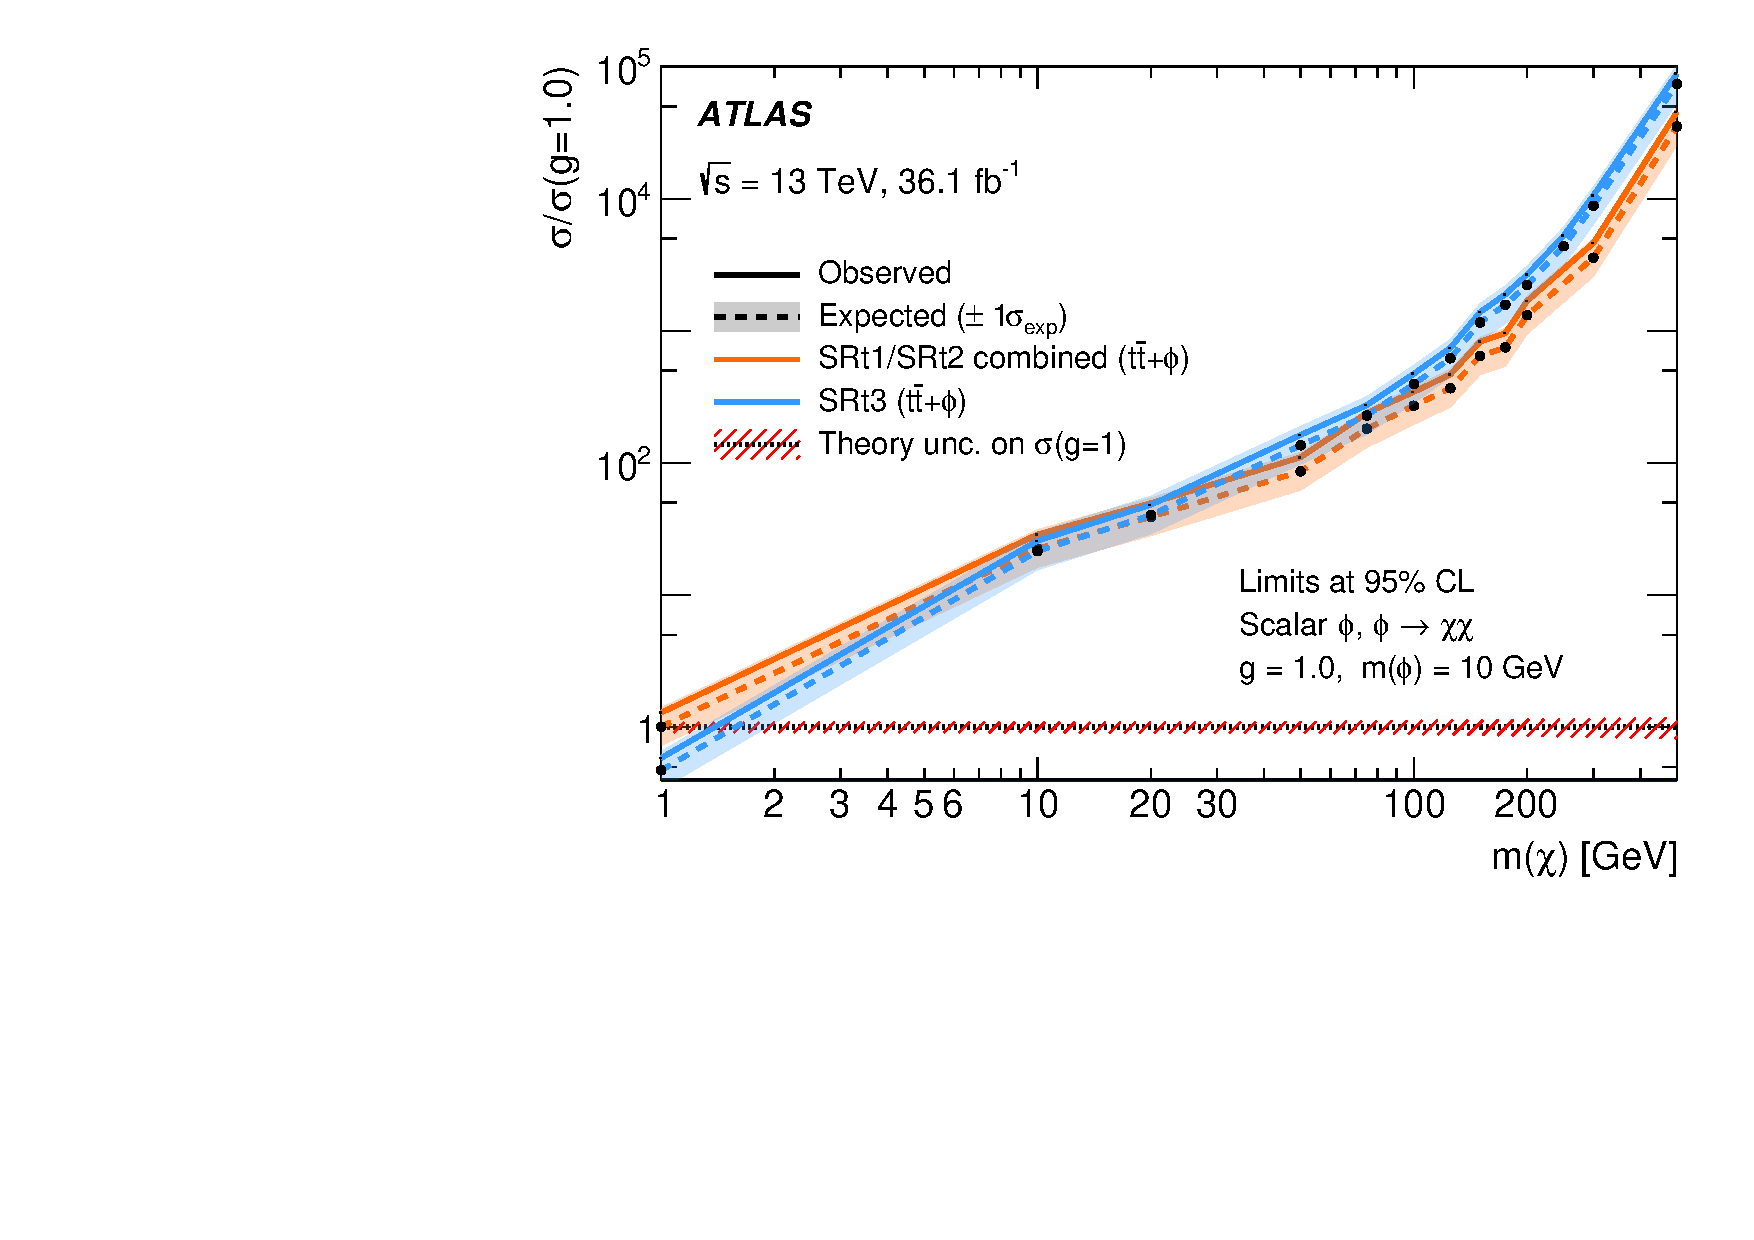
\includegraphics[width=.9\textwidth]{appA/final_scalar_SR1_offshell}}
			\subbottom[]{
				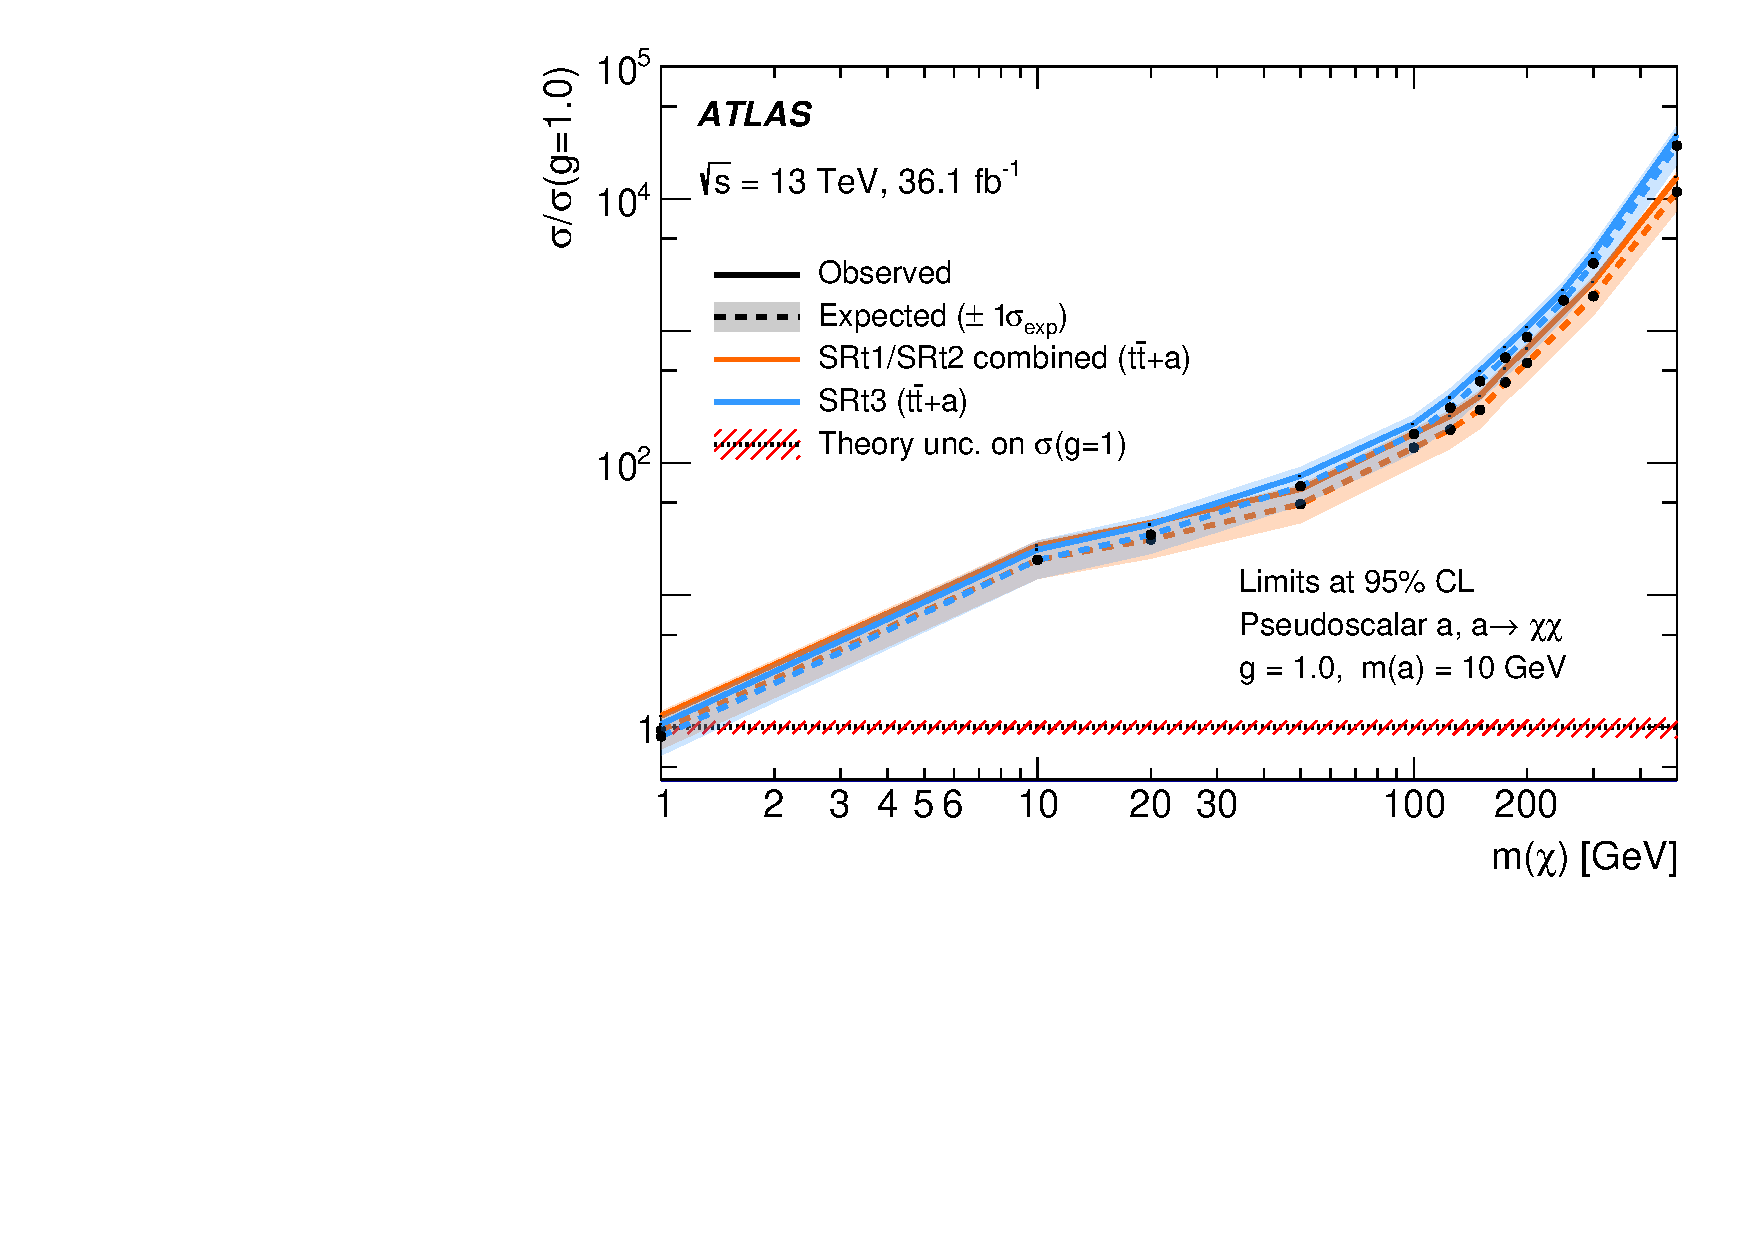
\includegraphics[width=.9\textwidth]{appA/final_pseudo_SR1_offshell}}
			\caption{Exclusion limits for colour-neutral $\ttbar+\phi$ scalar (a) and $\ttbar+a$ pseudoscalar (b)  models as a function of the DM mass for a mediator mass of $10\;\GeV$. The limits are calculated at 95\% CL and are expressed in terms of the ratio of the excluded cross-section to the nominal cross-section for a coupling assumption of $g = g_q = g_\chi = 1$, where $g_\chi$ is the DM–mediator coupling, and $g_q$ the flavour-universal SM–mediator coupling. The solid (dashed) lines shows the observed (expected) exclusion limits for the different signal regions, according to the colour code specified in the legend. To derive the results for the fully hadronic \ttbar\ final state the region SRt1 or SRt2 providing the better expected sensitivity is used (taken from~\cite{DMhf}.}
			\label{fig:dmresultschi}
		\end{figure}
        \chapter{Glossary}
\markboth{}{Glossary}

\begin{acronym}[UML]
	\acro{ALICE}{A Large Ion Collider Experiment}
	\acro{AOD}{Analysis Objects Data}
	\acro{ATLAS}{A Toroidal LHC ApparatuS}
	\acro{BDT}{Boosted Decisions Tree}
	\acro{BR}{Branching Ratio}
	\acro{BSM}{Beyond Standard Model}
	\acro{CERN}{European Organization for Nuclear Research}
	\acro{CKKW}{Catani-Krauss-Kuhn-Webber}
	\acro{CKM}{Cabibbo–Kobayashi–Maskawa}
	\acro{CL}{Confidence Level}
	\acro{CMS}{Compact Muon Solenoid}
	\acro{CM}{centre-of-mass}
	\acro{CPU}{Central Processing Unit}
	\acro{CR}{Control Region}
	\acro{CSC}{Cathode Strip Chamber}
	\acro{CTP}{Central Trigger Processor}
	\acro{DIS}{Deep Inelastic Scattering}
	\acro{DM}{Dark Matter}
	\acro{ECAL}{Electromagnetic Calorimeter}
	\acro{EM}{electromagnetic}
	\acro{ESD}{Event Summary Data}
	\acro{FCNC}{Flavour Changing Neutral Currents}
	\acro{FoM}{Figure of Merit}
	\acro{FSR}{Final State Radiation}
	\acro{FTF}{Fast Track Finder}
	\acro{FTK}{Fast TracKer}
	\acro{GUT}{Grand Unification Theory}
	\acro{HCAL}{Hadronic Calorimeter}
	\acro{HEP}{High-Energy Physics}
	\acro{HLT}{High Level Trigger}
	\acro{IBL}{Insertable B-Layer}
	\acro{ID}{Inner Detector}
	\acro{ISR}{Initial State Radiation}
	\acro{JES}{Jet Energy Scale}
	\acro{JER}{Jet Energy Resolution}
	\acro{JVT}{Jet vertex Tagger}
	\acro{L1}{Level-1}
	\acro{L1Calo}{L1 Calorimeter}
	\acro{L1Muon}{L1 Muon}
	\acro{L1Topo}{Level-1 Topological}
	\acro{LAr}{Liquid Argon}
	\acro{LEIR}{Low Energy Ion Ring}
	\acro{LEP}{Large Electron-Positron Collider}
	\acro{LH}{Likelihood}
	\acro{LHC}{Large Hadron Collider}
	\acro{LHCb}{Large Hadron Collider beauty}
	\acro{LHCf}{Large Hadron Collider forward}
	\acro{LINAC2}{Linear Accelerator 2}
	\acro{LINAC3}{Linear Accelerator 3}
	\acro{LO}{Leading Order}
	\acro{LS1}{Long Shut down 1}
	\acro{LSP}{Lightest Supersymmetric Particle}
	\acro{MC}{Monte Carlo}
	\acro{ME}{Matrix Element}
	\acro{MDT}{Monitored Drift Tube}
	\acro{MIP}{Minimum Ionising Particle}
	\acro{MLE}{Maximum Likelihood Estimation}
	\acro{MLM}{Michelangelo L. Mangano}
	\acro{MoEDAL}{Monopole \& Exotics Detector At the \ac{LHC}}
	\acro{MS}{Muon Spectrometer}
	\acro{MSSM}{Minimal Supersymmetric Standard Model} 
	\acro{MV2}{Multivariate algorithm} 
	\acro{NLO}{Next-to-Leading Order}
	\acro{NLSP}{Next to Lightest Supersymmetric Particle}
	\acro{OR}{Overlap Removal}
	\acro{PDF}{Parton Distribution Function}
	\acro{PLR}{Profile Likelihood Ratio}
	\acro{pMSSM}{Phenomenological \ac{MSSM}}
	\acro{PS}{Parton Shower}
	\acro{PSB}{Proton Synchrotron Booster}
	\acro{PV}{Primary Vertex}
	\acro{QCD}{Quantum Chromodynamics}
	\acro{QED}{Quantum Electrodynamics} 
	\acro{QFT}{Quantum Field Theory}
	\acro{RDO}{Raw Data Object}
	\acro{RJR}{Recursive Jigsaw Technique}
	\acro{RoI}{Region of Interest}
	\acro{ROS}{Read-Out System}
	\acro{RPC}{$R$-Parity Conserving}
	\acro{RPC}{Resistive-Plate Chamber}
	\acro{RPV}{$R$-Parity Violating}
	\acro{SCT}{SemiConductor Tracker}
	\acro{SF}{Scale Factor}
	\acro{SFOS}{Same Flavour Opposite Sign}
	\acro{SM}{Standard Model}
	\acro{SPS}{Super Proton Synchrotron}
	\acro{SR}{Signal Region}
	\acro{SUSY}{Supersymmetry}
	\acro{SV}{Secondary Vertex}
	\acro{TDAQ}{Trigger and Data Acquisition}
	\acro{TF}{Transfer Factor}
	\acro{TGC}{Thin-Gap Chamber}
	\acro{TOTEM}{TOTal cross section, Elastic scattering and diffraction dissociation Measurement at the \ac{LHC}}
	\acro{TRT}{Transition Radiation Tracker}
	\acro{UE}{Underlying Event}
	\acro{VEV}{Vacuum Expectation Value}
	\acro{VR}{Validation Region}
	\acro{WIMP}{Weakly Interacting Massive Particle}
	\acro{WP}{Working Point}
\end{acronym} 

% Acronyms

% Example of acronyms with mouse-over tooltip (only working with Acrobat Reader)
% \usepackage[tooltip]{acro}

% \DeclareAcronym{cd}{
%   short = {CD},
%   long  = {Compact Disc}
% }
% \DeclareAcronym{mc}{
%   short   = {MC},
%   long    = {Music Cassette},
%   tooltip = {my mouse-over text}
% }


% \begin{document}

%  \ac{cd} \ac{mc}\par\vspace{1cm}
%  \ac{cd} \ac{mc}

%  \aca{cd} \aca{mc}

%  \acs{cd} \acs{mc}

% \end{document}


    %---------------------------------------------------
    % BIBLIOGRAPHY
    %---------------------------------------------------
    \clearpage
    \phantomsection
    \addcontentsline{toc}{chapter}{Bibliography}
    \bibliography{Chapters/bibliography} 

%---------------------------------------------------
% END DOCUMENT
%---------------------------------------------------

\end{document}